\documentclass[a4paper,11pt]{report}

\usepackage{wrapfig}

% Custom command to indicate that something needs a reference
\newcommand{\refthis}{\textsuperscript{[reference this]}}

% Epigraph package and it's settings, used for quotes at the beginning of chapters
\usepackage{epigraph}
\setlength{\epigraphwidth}{.5\textwidth}
\renewcommand{\textflush}{flushright}

% Used to make the first paragraph of a section indented
\usepackage{indentfirst}

% Acronym glossary
\usepackage[utf8]{inputenc}
\usepackage[automake, acronym]{glossaries}
\makeglossaries
% A database of all acronyms used in the thesis. Format for declaring new acronyms is:
%     \newacronym{code}{acronym}{explanation}

%	%	%

\newacronym{AHCAL}{AHCAL}{Analogue Hadronic Calorimeter}

\newacronym{SDHCAL}{SDHCAL}{Semi-Digital Hadronic Calorimeter}

\newacronym{DAQ}{DAQ}{Data Acquisition}

\newacronym{DQM}{DQM}{Data Quality Monitoring}

\newacronym{DQM4hep}{DQM4hep}{Data Quality Monitoring for High-Energy Physics}

\newacronym{EDM}{EDM}{Event Data Model}

\newacronym{DESY}{DESY}{\textit{Deutches Elektronen-Synchrotron}}

\newacronym{CERN}{CERN}{\textit{Conseil europ\'{e}en pour la recherche nucl\'{e}aire}}

\newacronym{SM}{SM}{Standard Model}

\newacronym{BSM}{BSM}{Beyond the Standard Model}

\newacronym{QFT}{QFT}{Quantum Field Theory}

\newacronym{SUSY}{SUSY}{Supersymmetry}

\newacronym{MSSM}{MSSM}{Minimal Supersymmetric Standard Model}

\newacronym{CP}{CP}{Charge Parity}

\newacronym{LHC}{LHC}{Large Hadron Collider}

\newacronym{ATLAS}{ATLAS}{A Toroidal LHC Apparatus}

\newacronym{HL-LHC}{HL-LHC}{High Luminosity Large Hadron Collider}

\newacronym{ILC}{ILC}{International Linear Collider}

\newacronym{CLIC}{CLIC}{Compact Linear Collider}

\newacronym{FCC}{FCC}{Future Circular Collider}

\newacronym{CEPC}{CEPC}{Circular Electron Positron Collider}

\newacronym{LEP}{LEP}{Large Electron Positron Collider}

\newacronym{JINR}{JINR}{Joint Institute for Nuclear Research}

\newacronym{ILD}{ILD}{International Large Detector}

\newacronym{SiD}{SiD}{Silicon Detector}

\newacronym{AIDA}{AIDA}{Advanced Infrastructures for Detectors at Accelerators}

\newacronym{GUI}{GUI}{Graphical User Interface}

\newacronym{XML}{XML}{Extensible Markup Language}

\newacronym{JSON}{JSON}{Javascript Object Notation}

\newacronym{SiWECAL}{SiWECAL}{Silicon Tungsten Electronic Calorimeter}

\newacronym{CALICE}{CALICE}{Calorimeter for Linear Collider Experiment}

\newacronym{FLC}{FLC}{\textit{Forschung mit Lepton Collidern}}

\newacronym{EUDAQ}{EUDAQ}{EU [?] Data Acquisition}

\newacronym{BIF}{BIF}{Beam Interface}

\newacronym{SPS}{SPS}{Super Proton Synchrotron}

\newacronym{ADC}{ADC}{Analogue to Digital Conversion}

\newacronym{TDC}{TDC}{Time to Digital Conversion}

\newacronym{LCIO}{LCIO}{Linear Collider Input/Output}

\newacronym{MIP}{MIP}{Minimum Ionising Particle}

\newacronym{IDEA}{IDEA}{?IDEA?}

\newacronym{DWC}{DWC}{Delay Wire Chamber}

\newacronym{GEM}{GEM}{Gas Electron Multiplier}

\newacronym{SiPM}{SiPM}{Silicon Photomultipliers}

\newacronym{CSV}{CSV}{Comma-Separated Values}

\newacronym{TMVA}{TMVA}{Toolkit for Multi-Variate Analysis}

\newacronym{BDT}{BDT}{Boosted Decision Trees}

\newacronym{QCD}{QCD}{Quantum Chromodynamics}

\newacronym{QED}{QED}{Quantum Electrodynamics}

\newacronym{MC}{MC}{Monte Carlo}

\newacronym{PandoraPFA}{PandoraPFAs}{Pandora Particle Flow Algorithms}

\newacronym{PFO}{PFO}{Particle Flow Object}

\newacronym{DREAM}{DREAM}{Dual Readout Method}

\newacronym{SCRF}{SCRF}{Superconducting Radio Frequency}

\newacronym{IP}{IP}{Interaction Point}

\newacronym{IP-analysis}{IP}{Impact Parameter}

\newacronym{TPC}{TPC}{Time Projection Chamber}

\newacronym{ECAL}{ECAL}{Electromagnetic Calorimeter}

\newacronym{HCAL}{HCAL}{Hadronic Calorimeter}

\newacronym{MAPS}{MAPS}{Monolithic Active Pixel Sensor}

\newacronym{RPC}{RPC}{resistive plate chambers}

\newacronym{RF}{RF}{radio frequency}

\newacronym{TDR}{TDR}{Technical Design Report}

\newacronym{CDR}{CDR}{Conceptual Design Report}

\newacronym{SPPC}{SPPC}{Super Proton Proton Collider}

\newacronym{qtest}{qtest}{quality test}

\newacronym{CLICdp}{CLICdp}{CLIC Detector \& Physics}

% tikz settings
\usepackage{tikz}
\usetikzlibrary{quotes,angles,shapes,snakes,arrows,decorations.markings,decorations.pathmorphing,decorations.markings,decorations.text}
% tikz styles for Feynman diagrams
\tikzset{
    vector/.style={decorate, decoration={snake}, draw=black},
	provector/.style={decorate, decoration={snake,amplitude=2.5pt}, draw},
	antivector/.style={decorate, decoration={snake,amplitude=-2.5pt}, draw},
    fermion/.style={draw=black, postaction={decorate},
        decoration={markings,mark=at position .55 with {\arrow[draw=black]{>}}}},
    fermionbar/.style={draw=black, postaction={decorate},
        decoration={markings,mark=at position .55 with {\arrow[draw=black]{<}}}},
    fermionnoarrow/.style={draw=black},
    gluon/.style={decorate, draw=black,
        decoration={coil,amplitude=4pt, segment length=5pt}},
    scalar/.style={dashed,draw=black, postaction={decorate},
        decoration={markings,mark=at position .55 with {\arrow[draw=black]{>}}}},
    scalarbar/.style={dashed,draw=black, postaction={decorate},
        decoration={markings,mark=at position .55 with {\arrow[draw=black]{<}}}},
    scalarnoarrow/.style={dashed,draw=black},
    electron/.style={draw=black, postaction={decorate},
        decoration={markings,mark=at position .55 with {\arrow[draw=black]{>}}}},
     bigvector/.style={decorate, decoration={snake,amplitude=4pt}, draw},
     line/.style={decorate, draw=black},
}
% tikz styles used for flow diagrams
\tikzstyle{decision} = [diamond, draw, fill=blue!20, 
    text width=4.5em, text badly centered, node distance=3cm, inner sep=0pt]
\tikzstyle{block} = [rectangle, draw, fill=blue!20, 
    text width=8em, text centered, rounded corners, minimum height=4em, minimum width=8em]
\tikzstyle{line} = [draw, -latex']
\tikzstyle{cloud} = [draw, ellipse,fill=red!20, node distance=3cm,
    minimum height=2em]

% Mathematical symbols, etc.
\usepackage{amsmath}
\usepackage{amsfonts}
\usepackage{amssymb}
\usepackage{adjustbox}
\usepackage{sfmath}


%%%%%%%%%%%%%%%%%%%%%%%%%%%%
% University of Sussex thesis template
%%%%%%%%%%%%%%%%%%%%%%%%%%%%

%%%%%%%%%%%%%%%%%%%%%%%%%%%%
% LINE SPACING
\newcommand{\linespacing}{1.5}
\renewcommand{\baselinestretch}{\linespacing}
%%%%%%%%%%%%%%%%%%%%%%%%%%%%

%%%%%%%%%%%%%%%%%%%%%%%%%%%%
% BIBLIOGRAPHY STYLE
%\usepackage{natbib}
\usepackage{cite}
\bibliographystyle{unsrt}
%%%%%%%%%%%%%%%%%%%%%%%%%%%%

%%%%%%%%%%%%%%%%%%%%%%%%%%%%
% OTHER FORMATTING/LAYOUT DECLARATIONS
% Graphics
\usepackage{graphicx,color}
\usepackage[outdir=./]{epstopdf}
\usepackage[british]{babel}
% The left-hand-side should be 40mm.  The top and bottom margins should be
% 25mm deep.  The right hand margin should be 20mm.
% These are the original, intended and asymmetric values:
%		\usepackage[a4paper,top=2.5cm,bottom=2.5cm,left=4cm,right=2cm,headsep=10pt]{geometry}
% Below is the new values, which are preserve the space but make it symmetrical:
\usepackage[a4paper,top=2.5cm,bottom=2.5cm,left=3cm,right=3cm,headsep=10pt]{geometry}
\flushbottom
% Pages should be numbered consecutively thorugh the main text.  Page numbers
% should be located centrally at the top of the page.
\usepackage{fancyhdr}
\fancypagestyle{plain}{
	\fancyhf{}
	% Add "DRAFT: <today's date>" to header (comment out the following to remove)
	\lhead{\textit{DRAFT: \today}}
	%
	\chead{\thepage}
	\renewcommand{\headrulewidth}{0pt}
}
\pagestyle{plain}
%%%%%%%%%%%%%%%%%%%%%%%%%%%%

%%%%%%%%%%%%%%%%%%%%%%%%%%%%
% ANY OTHER DECLARATIONS HERE:

%%%%%%%%%%%%%%%%%%%%%%%%%%%%

%%%%%%%%%%%%%%%%%%%%%%%%%%%%
% HYPERREF
\usepackage[colorlinks,pagebackref,pdfusetitle,urlcolor=blue,citecolor=blue,linkcolor=blue,bookmarksnumbered,plainpages=false]{hyperref}
% For print version, use this instead:
%\usepackage[pdfusetitle,bookmarksnumbered,plainpages=false]{hyperref}
%\usepackage{backref}
%\renewcommand{\backrefpagesname}{Cited on}
%%%%%%%%%%%%%%%%%%%%%%%%%%%%

%%%%%%%%%%%%%%%%%%%%%%%%%%%%
% BEGIN DOCUMENT
\begin{document}
%%%%%%%%%%%%%%%%%%%%%%%%%%%%

%%%%%%%%%%%%%%%%%%%%%%%%%%%%
% PREAMBLE: roman page numbering i, ii, iii, ...
\pagenumbering{roman}
%%%%%%%%%%%%%%%%%%%%%%%%%%%%

%%%%%%%%%%%%%%%%%%%%%%%%%%%%
%% TITLE PAGE: The title page should give the following information:
%%	(i) the full title of the thesis and the sub-title if any;
%%	(ii) the full name of the author;
%%	(iii) the qualification aimed for;
%%	(iv) the name of the University of Sussex;
%%	(v) the month and year of submission.
\thispagestyle{empty}
\pdfbookmark[0]{Title page}{title_page}
\begin{center}

\includegraphics[width=6cm]{../Pictures/uslogonew.eps}
\vskip40mm
% TITLE
\huge\textbf{Data acquisition software development and physics studies for future $e^+e^-$ colliders}
%\huge\textbf{Datblygiad o feddalwedd amlyniad data ac astudiathau ffiseg ar gyfer gwrthdarwyr $e^+e^-$ dyfodol}
\vskip5mm
% AUTHOR
\Large\textbf{Tom Coates}
\normalsize
\end{center}
\vfill
\begin{flushleft}
\large
% QUALIFICATION
Submitted for the degree of Doctor of Philosophy \\
University of Sussex	\\
% DATE OF SUBMISSION
June 2019
\end{flushleft}		
%%%%%%%%%%%%%%%%%%%%%%%%%%%%

%%%%%%%%%%%%%%%%%%%%%%%%%%%%
% DECLARATIONS
\chapter*{Declaration}
\pdfbookmark[0]{Declaration}{declaration}
I hereby declare that this thesis has not been and will not be submitted in whole or in part to another University for the award of any other degree.

% ADDITIONAL DECLARATIONS HERE (IF ANY)

\vskip5mm
Signature:
\vskip20mm
% AUTHOR
Tom Coates
%%%%%%%%%%%%%%%%%%%%%%%%%%%%

%%%%%%%%%%%%%%%%%%%%%%%%%%%%
% SUMMARY PAGE
\thispagestyle{empty}
\newpage
\null\vskip10mm
\begin{center}
\large
\underline{UNIVERSITY OF SUSSEX}
\vskip20mm
% AUTHOR, QUALIFICATION
\textsc{Tom Coates, Doctor of Philosophy}
\vskip20mm
% TITLE
\begin{center}
	\scshape
	\underline{Data acquisition software development and physics studies for}
	\underline{future $e^+e^-$ colliders}
\end{center}
\vskip0mm
\vskip20mm
\underline{\textsc{Summary}}
\vskip2mm
\end{center}
% Change line spacing
\renewcommand{\baselinestretch}{1.0}
\small\normalsize
% SUMMARY HERE (300 word limit for most subjects):
[Summary text] [Max. 300 words for most subjects]
%%%%%%%%%%%%%%%%%%%%%%%%%%%%

%%%%%%%%%%%%%%%%%%%%%%%%%%%%
% ACKNOWLEDGEMENTS

\chapter*{Acknowledgements}
%\chapter*{Acknowledgements}

% Academic
I'd first like to thank my supervisor Fabrizio Salvatore, for being exactly as hands-on and hands-off as I needed, when I needed it, and without whose help, guidance and faith I wouldn't have been able to do this. Thanks to all at the FLC group at DESY in Hamburg, but especially to Katja Kr\"{u}ger, Adrian Irles-Quiles (now at LAL Orsay), and R\'{e}mi Et\'{e}. Also thanks to the members of the IDEA collaboration, especially Romualdo Santoro. Thanks also the CLIDdp collaboration, but especially Yixuan Zhang and Victoria Martin. \newline

% Funding
I would like to thank the UK's Science and Technology Funding Council for supporting my studentship and providing me with the funding to perform this research. Thanks also to Linear Collider UK for providing vital funding for travel for the linear collider community in the UK. \newline

% AIDA-2020
I would also like to thank the whole AIDA-2020 collaboration for providing the working environment for a large portion of the work of this thesis and always scheduling their annual meetings in sunny countries with good food. Special thanks to all of the members of Work Package 5 for their support and expertise, and to David Cussans and Matthew Wing for their leadership and organisation of the activities within the group.

Similarly, I would like to thank all of the organisers of the Beam Telescopes and Test Beams workshop for providing a forum for researchers to discuss our work and learn from each other. \newline

% Personal
Finally, thanks to my highschool physics teachers Mr Coombes and Mr Thomas, who nurtured my early love for physics. I'd like to take this opportunity to apologise for never doing my homework, and hope that this thesis makes up for it.

\pdfbookmark[0]{Acknowledgements}{acknowledgements}
\renewcommand{\baselinestretch}{\linespacing}
\small\normalsize

%%%%%%%%%%%%%%%%%%%%%%%%%%%%

%%%%%%%%%%%%%%%%%%%%%%%%%%%%
% TABLE OF CONTENTS, LISTS OF TABLES & FIGURES
\newpage
\pdfbookmark[0]{Contents}{contents_bookmark}
\tableofcontents
%\listoftables
%\phantomsection
%\addcontentsline{toc}{chapter}{List of Tables}
%\listoffigures
%\phantomsection
%\addcontentsline{toc}{chapter}{List of Figures}
%%%%%%%%%%%%%%%%%%%%%%%%%%%%

%%%%%%%%%%%%%%%%%%%%%%%%%%%%
% MAIN THESIS TEXT: arabic page numbering 1, 2, 3, ...
\newpage
\pagenumbering{arabic}
%%%%%%%%%%%%%%%%%%%%%%%%%%%%

\chapter{Introduction} 
\label{chapter:intro}

%\epigraph{Teaching man his relatively small sphere in creation, it also encourages him by its lessons of the unity of Nature.}{Annie Jump Cannon}{\setlength{\epigraphwidth}{.25\textwidth}}

[...]

\section{The Standard Model}
[...]

\section{The Higgs Boson}
[...]

\section{CP violation in the Higgs sector}
[...]

\section{Data acquisition software and testbeams}
[...]

\chapter{Future Colliders}
\label{chapter:colliders}

\epigraph{Progress is not a straight line.}{An Wang}

In the post-LHC era, particle physics is at somewhat of an impasse. \acrfull{SM} has held up to most experiments and observation, and its predictive power is now exhausted. There are tantalising hints at a theory beyond the Standard Model -- in the form of CP-violation and dark matter -- but as of yet all new ways to probe the \acrshort{SM} for its weaknesses, to see the greater theory behind it, have yielded very little. 

There are many planned investigations to attempt to identify physics \acrlong{BSM} that use the \acrfull{LHC}, or plan to leverage the upgrades for the \acrfull{HL-LHC}. However, now that the Higgs boson has been identified successfully, one of the most fruitful avenues for further research is the construction and operation of a lepton collider at the energy frontier, with sufficient centre-of-mass energy to produce Higgs bosons in large numbers.

This is what motivates the several proposals for future lepton colliders around the world today, that would operate to complement and expand the reach of particle physicists beyond what the \acrshort{LHC} is currently capable of. These proposed lepton colliders are broadly split into two groups: linear colliders and circular colliders. 

Linear colliders use two accelerator arms pointed towards a single interaction point, and in general are capable of high centre-of-mass energies thanks to developments in accelerator technologies. The main candidates for this style of collider are the \acrfull{ILC} and the \acrfull{CLIC}. 

Circular colliders use a similar layout to the \acrshort{LHC}, with a circular accelerator capable of creating collisions at multiple different interaction points around the circumference of the ring, which permits multiple detectors. The downsides of a circular collider are that lighter particles like electrons are more prone to energy losses via synchrotron radiation, limiting the centre-of-mass energies that a circular lepton collider can operate at. However, in exchange they tend to have much higher luminosities, allowing greater numbers of collisions and higher yields of certain processes or channels. The main candidates for circular colliders are the \acrfull{FCC} and the \acrfull{CEPC}. 

These proposed colliders share many of the same motivations, design considerations, features, and challenges, as does the ongoing international effort in research and development to make these colliders a reality.

\section{The physics case for a lepton collider}
With the observation of a Higgs boson with a mass of 125 GeV, based on data from the \acrlong{LHC}, the Standard Model of particle physics is now functionally complete. All of it's major predictions have been observed. This is a testament to it's quality as a theory, where it's predictive power and accuracy is one of the best in all of the sciences.

But despite this, a multitude of observations have shown that the Standard Model cannot be a complete theory of nature. Many phenomena have been observed that the Standard Model cannot predict, or that don't seem to interact with the Standard Model in any way.

In the post-LHC era, particle physicists are now forced to seek answers to three questions that the Standard Model cannot solve:

\begin{itemize}
	\item What is dark matter? Astrophysics observations support the existence of a neutral, weakly-interacting substance that composes around 85\% of all mass in the universe. Yet this substance cannot be explained by any known form of matter, and is completely unprecedented by the Standard Model.
	\item Why is there so little antimatter? The symmetries inherent in the Standard Model predict that the Big Bang would have created an equal quantity of matter and antimatter. Yet the universe today is dominated by matter.
	\item Why does the Higgs field fill space and give mass to elementary particles? The existence of the Higgs field and the coupling of the Higgs boson to other particles can be understood from the Standard Model but their origin or cause is still unexplained.
\end{itemize}

In order to answer these questions, new theories of physics Beyond the Standard Model (\acrshort{BSM}) have been made, and need to be experimentally tested. To do this, particle collider experiments at the energy frontier are needed. The \acrfull{LHC} has already been used extensively in searches for new physics, in the forms of new particles, rare and exotic decays, supersymmetry, and dark matter.

However, the running of a lepton collider at the energy frontier would be complementary to the \acrshort{LHC}'s continuing physics programme -- there are many events or channels that are inaccessible or difficult to examine in one environment that are much simpler or higher precision in the other. In this way, a lepton collider would help to improve and refine measurements already taken at the \acrshort{LHC}, while also allowing physicists to examine new channels and decays that were not accessible to it. A number of processes and their discovery potential can be seen in Table \ref{table:colliders/physics-goals}.

This follows a historical pattern in particle physics -- as the energy frontier advances, hadron colliders are used to discover new physics and new phenomena, followed by lepton colliders to examine these phenomena in higher precision.

\subsection{Higgs physics}
Of specific interest to searches at lepton colliders would be the Higgs boson itself. Many \acrshort{BSM} models predict differences from the Standard Model in the Higgs sector -- such as several Higgs bosons with different masses, composite Higgs, charged Higgs etc. The comparatively `quiet' environment of a lepton collider allows higher precision measurements of the properties of the Higgs boson, placing better constraints on the presence of new physics. In addition, lepton colliders can easily operate at specific thresholds and ``hot spots'' for Higgs production, permitting a much greater number of events yielding Higgs bosons, and thus a greater sample to examine.

% First confirmation of h->bb decays paper: https://atlas.web.cern.ch/Atlas/GROUPS/PHYSICS/CONFNOTES/ATLAS-CONF-2018-036/
Additionally, the most common decay of the Higgs boson, at a branching ratio of 57.7\%, is the $H \rightarrow b \overline{b}$ process. Despite the high branching ratio, the huge \acrshort{QCD} backgrounds in a hadron collider have made this decay incredibly difficult to observe at the LHC -- in fact, the $H \rightarrow b \overline{b}$ decay has only fairly recently been experimentally verified by the \acrshort{ATLAS} experiment. However, in a lepton collider these \acrshort{QCD} backgrounds are significantly smaller, meaning this decay channel is much easier to analyse, opening up a huge number of Higgs events for analysis and examination.

Another highly interesting process uniquely accessible to lepton colliders is the higgstrahulung reaction: $e^+ e^- \rightarrow Zh$. The decay of the Z boson into lepton pairs $e^+ e^-$ or $\mu^+ \mu^-$ allows high precision kinematic measurements of the process without directly measuring the Higgs boson itself. This allows unprecedented measurement of the Higgs mass, while also making measurements of missing energy possible. If the Higgs boson has invisible decays -- such as dark matter particles or other undiscovered particles that don't couple to the \acrshort{SM} -- the higgstrahlung process allows their existence to be identified.

[...] [High precision and model-independent measurement of the total rate of Higgs decay $\Gamma\textsubscript{h}$]

[...] [Top-Higgs Yukawa coupling, which is highly sensitive to new physics, since it's the strongest Higgs coupling]

\subsection{Top physics}
In addition to the Higgs, the top quark is of high interest to possible physics programmes at a future lepton collider. Since it's discovery at Fermilab in 1995, there have been no lepton colliders operating with sufficient energy to produce top quarks -- unlike the charm and bottom quarks, which were studied in further detail in lepton colliders after their discovery in hadron machines. The production threshold for top quarks is 350 GeV, and no lepton colliders capable of this energy have been constructed, meaning that the advantages of a lepton collider have never been utilised to understand the top quark in greater detail. 

The detailed study of top quarks and their properties that would be made possible by a lepton collider would have many benefits, primarily in the precision of the measurements. Similar to the Higgs, low \acrshort{QCD} backgrounds make reconstruction of top quark events easier to reconstruct. The fact that the collision is between elementary particles, rather than a parton-parton collision as in a hadron collider, also permits are more well-defined centre of mass energy, which is not possible in hadron colliders.

Precision measurements of the top quark is an important test of the \acrshort{SM} -- many \acrshort{BSM} models envision their additional particles as partners of the top quark. The upshot of this is that because of this, these theories propose properties of the top quark that diverge from the SM. In-depth and precise analysis of the top quark's properties would place limits on these theories, in turn allowing the development of better theories. 

[...] [$t \overline{t}$ production threshold studies -- these form an idealised QCD system to study, possibly also a $t \overline{t}$ bound state]

\begin{table}[h]
\centering
	\begin{tabular}{ c | c | c }
	\hline \hline
	\textbf{Energy} & \textbf{Reaction} & \textbf{Physics goal} \\ \hline
	 91 GeV & $e^+ e^- \rightarrow Z$ & ultra-precision electroweak \\ \hline
	 160 GeV & $e^+ e^- \rightarrow WW$ & ultra-precision W mass \\ \hline
	 250 GeV & $e^+ e^- \rightarrow Zh$ & precision Higgs coupling \\ \hline
	 350-500 GeV & $e^+ e^- \rightarrow t\overline{t}$ & top quark mass and couplings \\
	   & $e^+ e^- \rightarrow WW$ & precision W coupling \\
	   & $e^+ e^- \rightarrow \nu \overline{\nu} h$ & precision Higgs coupling \\ \hline
	 500 GeV & $e^+ e^- \rightarrow f \overline{f}$ & precision search for $Z^\prime$ \\
	   & $e^+ e^- \rightarrow t \overline{t}h$ & Higgs coupling to top \\
	   & $e^+ e^- \rightarrow Zhh$ & Higgs self-coupling \\
	   & $e^+ e^- \rightarrow \widetilde{\chi} \widetilde{\chi}$ & search for supersymmetry \\
	   & $e^+ e^- \rightarrow AH, H^+, H^-$ & search for extended Higgs states \\ \hline
	 700-1000 GeV & $e^+ e^- \rightarrow \nu \overline{\nu} hh$ & Higgs self-coupling \\
	   & $e^+ e^- \rightarrow \nu \overline{\nu} VV$ & composite Higgs sector \\
	   & $e^+ e^- \rightarrow  \nu \overline{\nu} t \overline{t}$ & composite Higgs and top \\
	   & $e^+ e^- \rightarrow \tilde{t} \tilde{t}^*$ & search for supersymmetry \\ \hline
	\end{tabular}
	\caption{Physics processes of interest at lepton colliders up to 1 TeV.}
	\label{table:colliders/physics-goals}
\end{table}

\section{The International Linear Collider}
The \acrfull{ILC} is a proposed high-luminosity linear electron-positron collider based upon 1.3 GHz superconducting radio frequency (\acrshort{SCRF}) accelerating technology. The ILC would have a centre of mass energy $\sqrt{s}$ of 250 GeV, upgradable to 500 GeV and then to 1 TeV at a later date. The total footprint of the complex would be 31km in length, with the arms using magnets with an accelerating gradient of 31.5 MVm\textsuperscript{-1} in metre-long superconducting nine-cell niobium cavities operating at 2K.

There were a number of proposed sites for the \acrshort{ILC}, including \acrshort{CERN} in Geneva, \acrshort{DESY} in Hamburg, and \acrshort{JINR} near Moscow. The most recent country to seek to host the collider was Japan, who proposed a greenfield site located in the Kitakami Highlands region of Iwate prefecture. 

However, a report from the Science Council of Japan (a representative organisation of the Japanese science community) released in early 2019 expressed that they had not reached a consensus as to whether to support hosting the ILC in Japan. Some  of the reasons cited were concerns over international cost-sharing in the long-term, as well as whether the expected scientific outcomes would justify the unprecedented human resource requirements and infrastructure necessary to make the \acrshort{ILC} a reality \cite{linearcolliders-scj-report}.

%Reference (24/04/2019): http://www.linearcollider.org/content/decision-international-linear-collider-“not-what-we-had-hoped-progress-nevertheless” 
On 7th March 2019, the Japanese government expressed that it would not make a proposal to host the collider in Japan. The Japanese government did however express interest in the \acrshort{ILC}, and declared that it would be continuing discussion and interest in the project as a whole.

%-Beam polarisation allows a high rate of higgstrahlung processes, and thus a high number of Higgs events to examine

%One of the unique features of the \acrshort{ILC} is the ``push-pull'' detector system. This is a moving platform in the chamber housing the interaction point, upon which two detectors can be mounted. The platform can be moved to change which detector is in the interaction point, allowing a linear collider to function with multiple detectors. This allows the two detectors to specialise for different physics studies and goals, much like the various experiments at the \acrshort{LHC} at \acrshort{CERN}, which would normally not be possible with a linear collider.

\subsection{ILC detectors}
Detector design for the \acrshort{ILC} is driven by the requirements of the physics programme -- many of the physics goals and targeted processes are highly dependent upon hadronic states, so precise jet reconstruction and high jet energy resolution is critical to meeting the expectations placed upon the \acrshort{ILC}. 

The only technique thought to be capable of delivering the necessary level of accuracy is \textit{particle flow}. Particle flow is an integrated approach which uses algorithms to examine the flow of energy through all parts of the detector to correlate different signals together to generate particle flow objects (\acrshort{PFO}s). The requirements for the use of particle flow is a very good separation of charged and neutral particles, translating into a need for high-efficiency trackers, and calorimeters capable of high-efficiency reconstruction of neutral particles. The design of the detectors for the \acrshort{ILC} has proceeded from these requirements.

The need for large separations between charged and neutral particles requires that the vertex detector, tracker, and calorimeter systems are contained within a magnetic field, so that charged particles' path is curved by the field. In general, this separation depends on the physical size of the detector and the strength of the magnetic field. Thus there are essentially two basic approaches to detector design: a large detector with a lower magnetic field, using the size of the detector to separate charged particles from neutral particles; or a more compact detector utilising a much stronger magnetic field to create the same separation.

These two approaches are shown in the two detector concepts for the \acrshort{ILC} -- the \acrlong{ILD} using a 3.5T magnetic field, and the more compact \acrlong{SiD} using a much stronger 5T magnetic field. These two detectors will be discussed in detail below.

\subsubsection{The International Large Detector (ILD)}
% https://indico.cern.ch/event/765096/contributions/3295752/attachments/1785276/2906298/ILD_European_Strategy_Document.pdf
% Paper on Particle Flow: https://arxiv.org/pdf/0907.3577.pdf

The \acrfull{ILD} is a detector concept for the \acrshort{ILC} intended as a multi-purpose detector, with a strong focus on optimising the performance of particle flow algorithms as much as possible. To attain this, it uses several technologies for very high-resolution and high-efficiency tracking, as well as highly-granular calorimeters.

For vertex tracking, the \acrshort{ILD} uses three double-layers of pixel detectors using monolithic active pixel sensor (\acrshort{MAPS}) technology, with a spatial resolution of 4 $\mu m$ and a timing resolution of 2-4 $\mu s$. For tracking, the \acrshort{ILD} uses a hybrid system, combining a gaseous time projection chamber (\acrshort{TPC}) with silicon detector layers placed both inside and outside the \acrshort{TPC} volume. This combination allows a high tracking efficiency with a low material usage.

The calorimeter system must be highly granular in order to best utilise particle flow. The calorimeters are split into the electromagnetic calorimeter (\acrshort{ECAL}) and hadronic calorimeter (\acrshort{HCAL}). The \acrshort{ECAL} utilises a silicon diode sampling calorimeter with diode pads of 5 $\times$ 5 mm\textsuperscript{2}. An option for an ECAL using thin scintillator strips is also being investigated. The \acrshort{HCAL} has two possible options available. The \acrfull{AHCAL} uses silicon photomultipliers (\acrshort{SiPM}) on tiles of plastic scintillator with a resolution of 3 $\times$ 3 cm\textsuperscript{2} using a fully analogue readout. The \acrfull{SDHCAL} uses \acrfull{RPC} with a higher granularity of 1 $\times$ 1 cm\textsuperscript{2}, but does not use a fully analogue output, meaning that amplitude information is more limited. 

These detectors are placed within a solenoid capable of generating a 3.5T magnetic field, and then within an iron flux return yoke which is instrumented for muon identification and tail catching, as well as providing structural support for the detector. The finished ILD is expected to weigh 14,000 metric tonnes.

%% Image found here: http://cds.cern.ch/record/2637370/plots
%\begin{figure}[h]
%	\centering
%	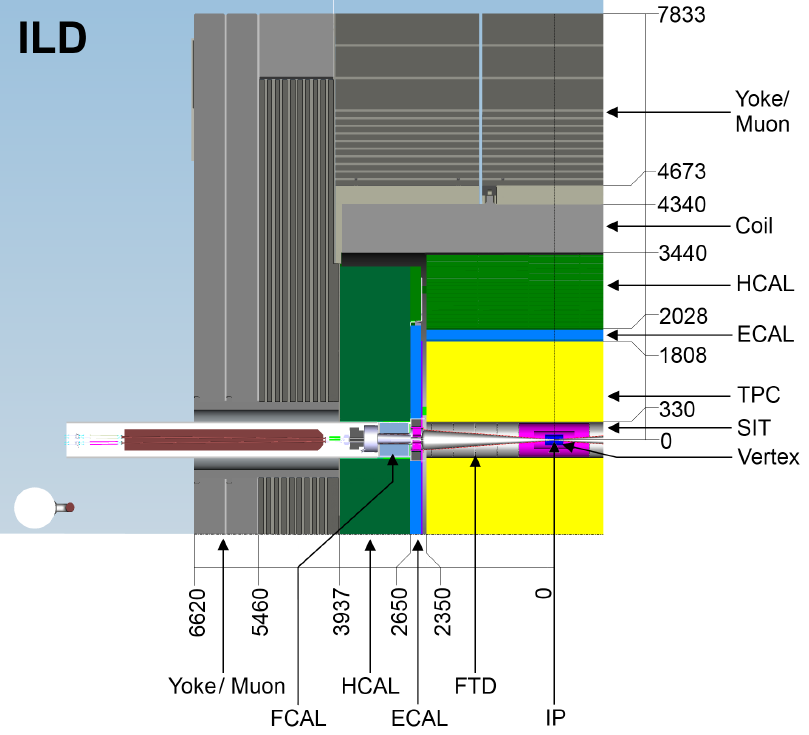
\includegraphics[width=0.75\textwidth]{../Pictures/ILDQuadrantView.png}
%	\caption{Quadrant view of the \acrshort{ILD} components.}
%	\label{figure:colliders/ILD/ILD-quadrant}
%\end{figure}
%
%% Image found here: https://flc.desy.de
%\begin{figure}[h]
%	\centering
%	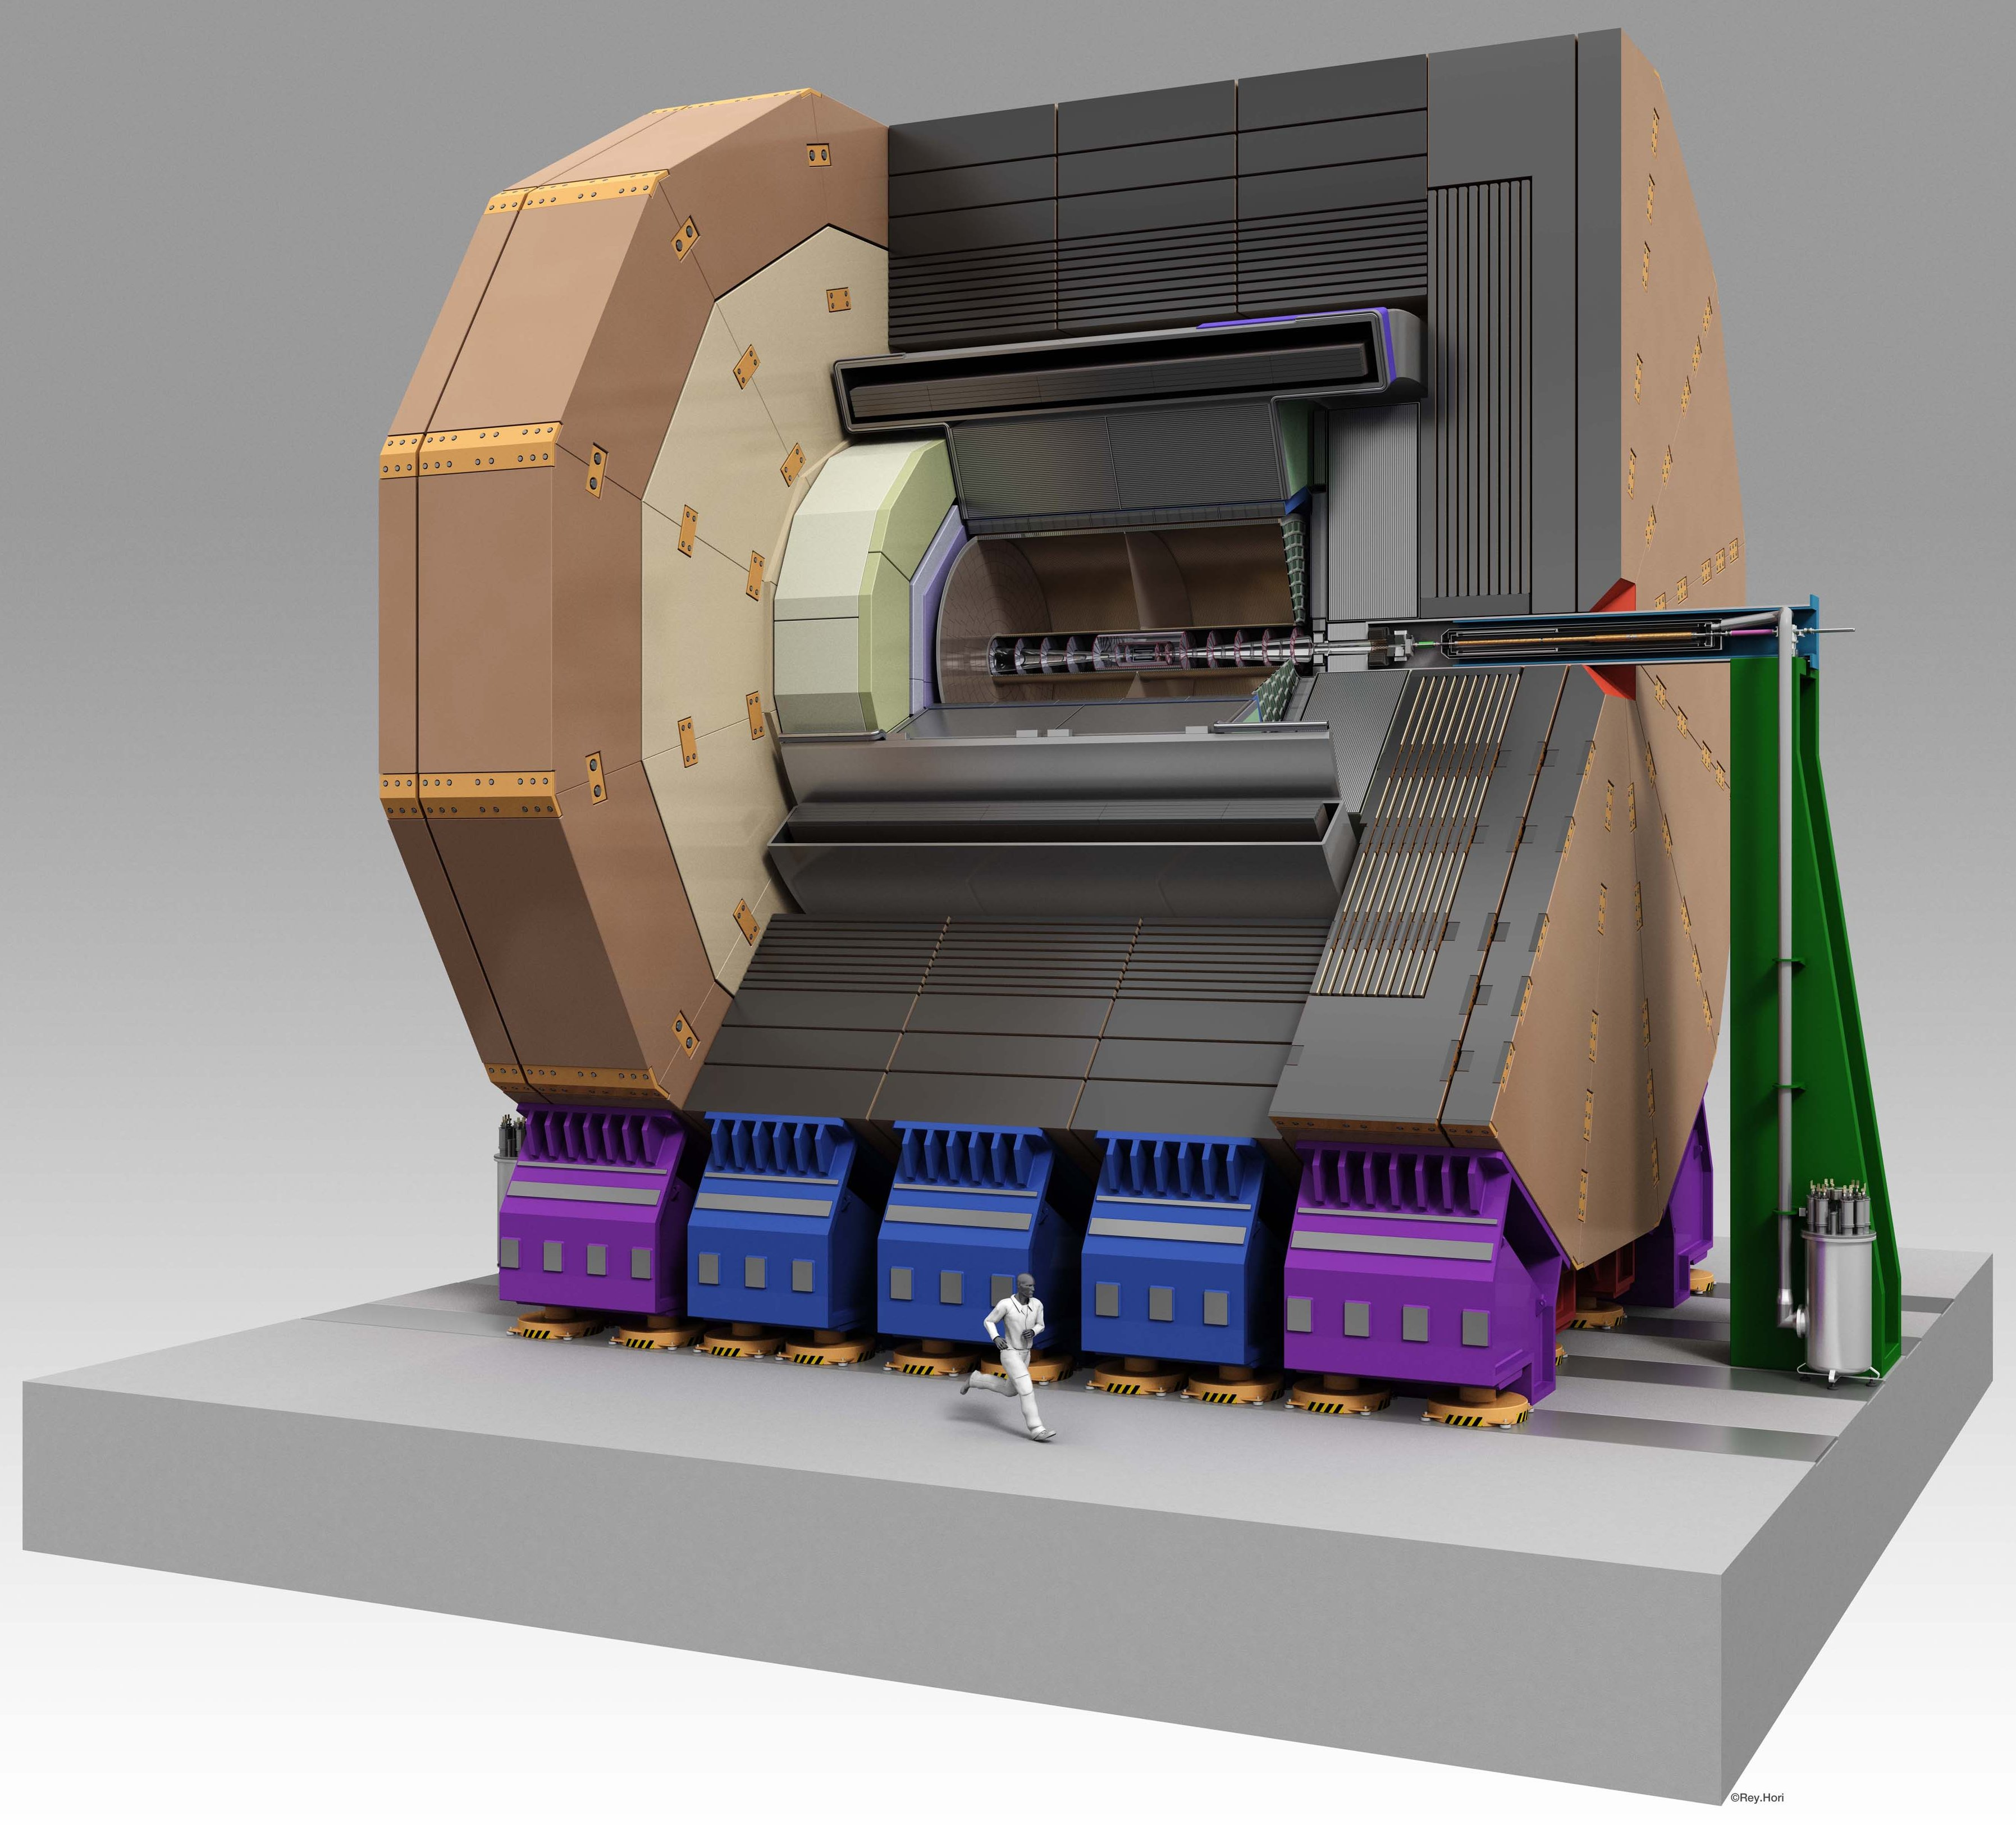
\includegraphics[width=0.75\textwidth]{../Pictures/ILDCutaway.jpg}
%	\caption{Rendering of the finished \acrshort{ILD}, cutaway to show the interal features, with human for scale.}
%	\label{figure:colliders/ILD/ILD-cutaway}
%\end{figure}

\begin{figure}[h]%
	\centering
    \subfloat{{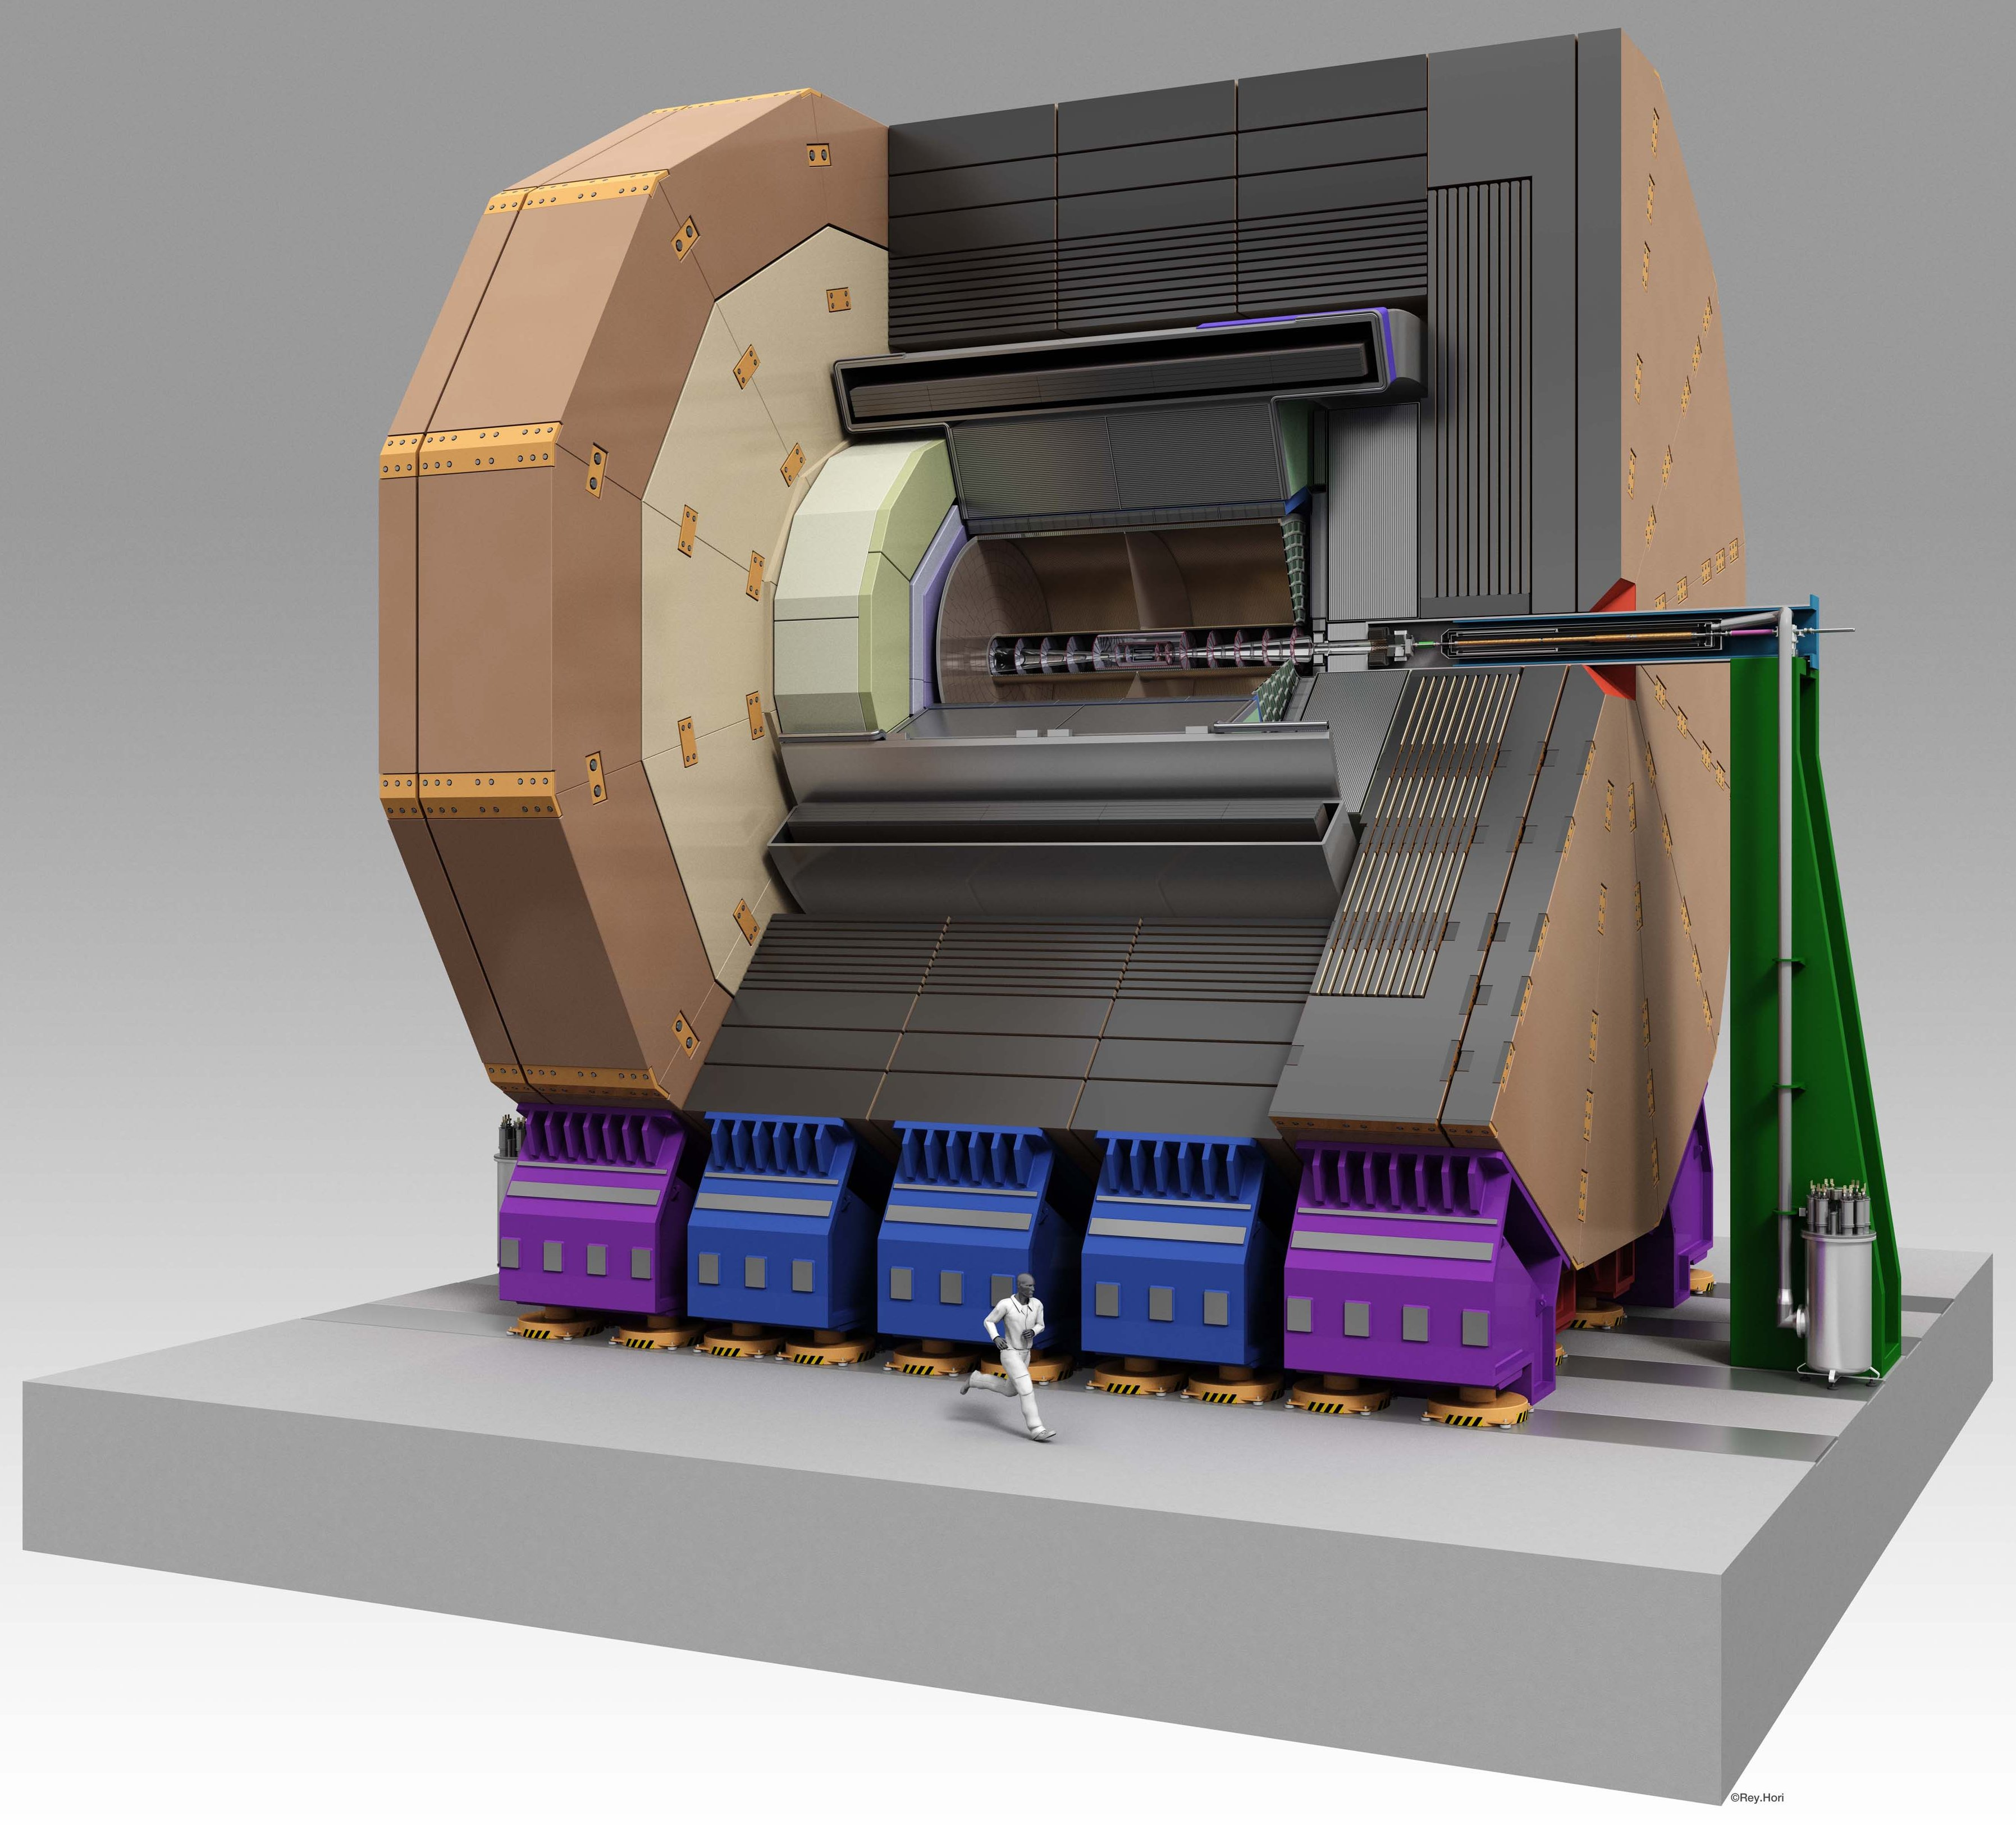
\includegraphics[width=0.45\textwidth]{../Pictures/ILDCutaway.jpg} }}%
    \qquad
	\subfloat{{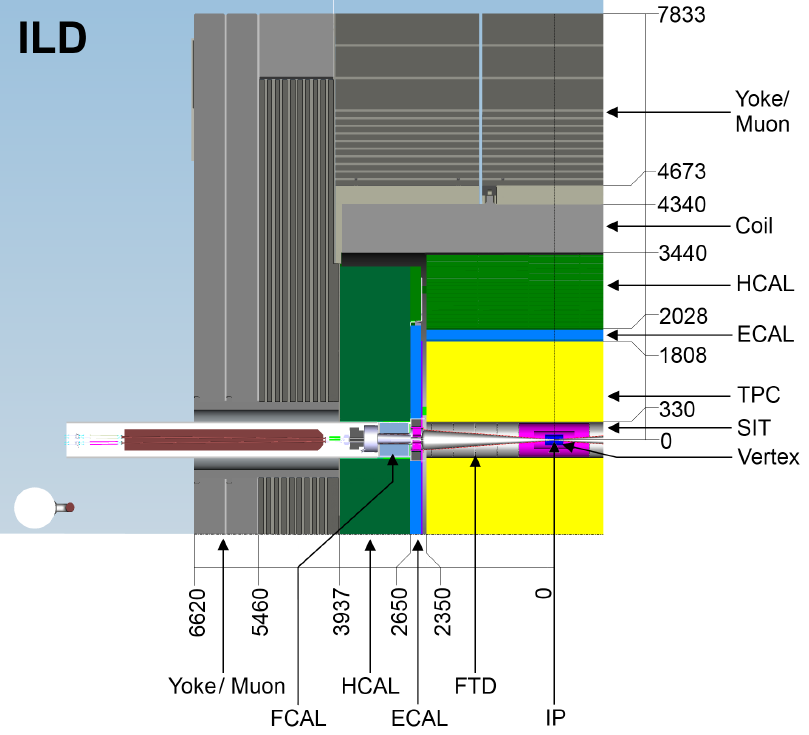
\includegraphics[width=0.45\textwidth]{../Pictures/ILDQuadrantView.png} }}%
    \caption{Rendering of the finished \acrshort{ILD} cutaway to show the interal features (left); and a quadrant view of the \acrshort{ILD} components (right).}%
    \label{figure:colliders/ILD/double}%
\end{figure}

\begin{figure}[h]
	\centering
	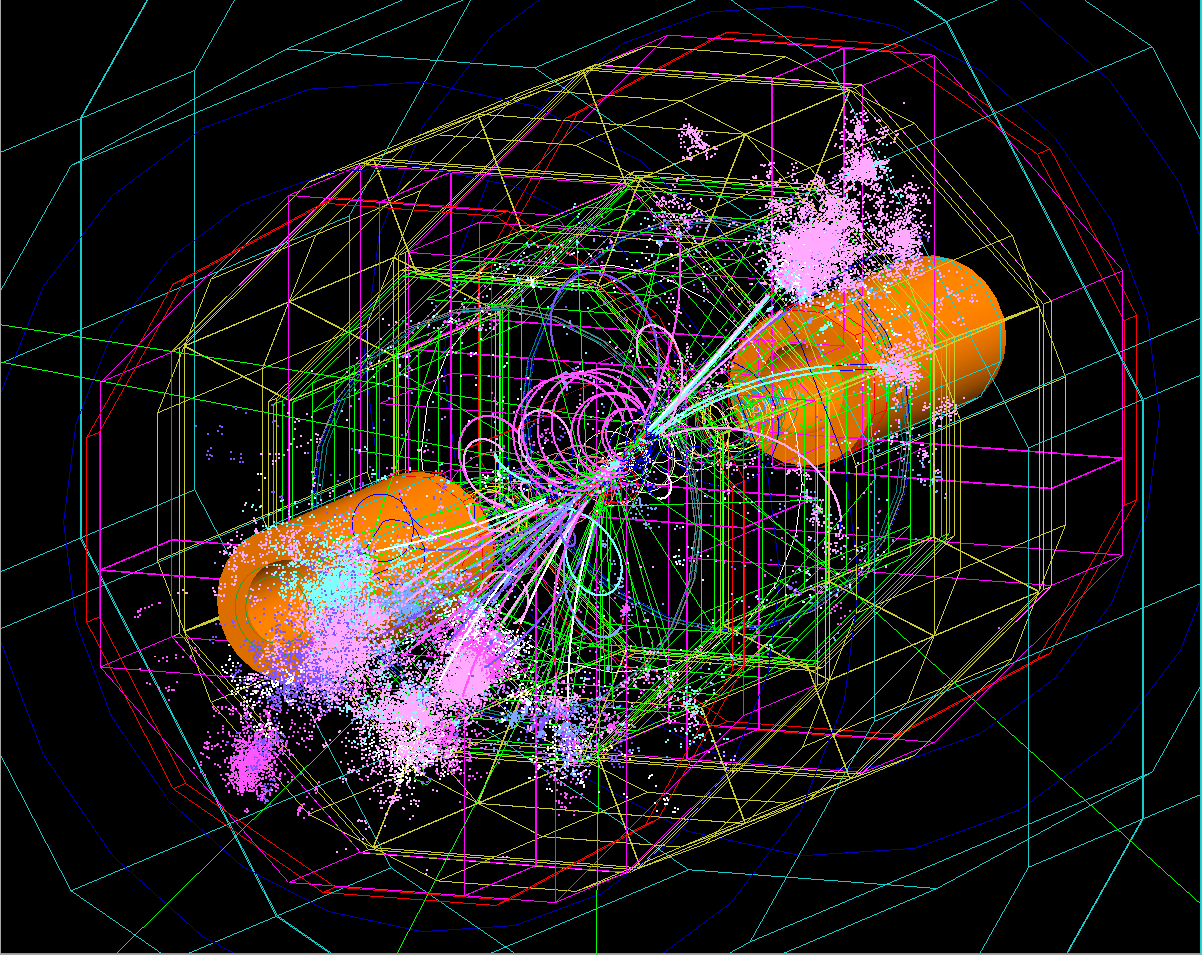
\includegraphics[width=0.75\textwidth]{../Pictures/SimulatedEvent1.png}
	\caption{Visualisation of a simulated $e^+ e^- \rightarrow t \overline{t} h$ event in the \acrshort{ILD}. Charged particles can be easily identified by the curved or spiral paths they take within the magnetic field, and the jets are visible as the light pink and purple areas near the beampipes on either side.}
	\label{figure:colliders/ILD/tth-simulation}
\end{figure}

\subsubsection{The Silicon Detector (SiD)}
The \acrfull{SiD} is a detector concept for the \acrshort{ILC} that uses primarily silicon-based technology, with the aim to reduce cost while still maintaining high performance and attaining the \acrshort{ILC}'s physics goals. The \acrshort{SiD} is also more compact than the \acrshort{ILD}, utilising a stronger magnetic field to compensate.

The vertex and tracker systems are both composed of silicon sensors, using a cylindrical configuration. The vertex uses silicon pixel sensors while the tracker uses silicon strip sensors, both designed to be used with power pulsing -- the electronics are only powered and active when it is known that bunches will be colliding. This reduces power and cooling requirements. 

The high-granularity calorimeters are both nested within the barrel, inside the magnetic field. The \acrshort{ECAL} uses thirty alternating layers of tungsten absorber and silicon active layers, in 3.5 $\times$ 3.5 mm\textsuperscript{2} hexagonal pixels. The \acrshort{HCAL} uses alternating layers of steel absorber and a glass resistive plate chamber, with cells of 10 $\times$ 10 mm\textsuperscript{2}

Outside of the calorimeter, the superconducting solenoid generates a 5T magnetic field, which enables the more compact detector design -- a higher magnetic field increases the spatial separation between charged and neutral particles, which is necessary for usage of particle flow algorithms.

Outside of the magnetic field is an iron flux return yoke, which similarly to the \acrshort{ILD} concept also acts as a strucutural support and is instrumented for muon identification and tail catching. 

\begin{figure}[h]%
	\centering
    \subfloat{{
\includegraphics[width=0.45\textwidth]{../Pictures/Placeholder.png} }}%
    \qquad
	\subfloat{{
\includegraphics[width=0.45\textwidth]{../Pictures/Placeholder.png} }}%
    \caption{Isometric view of the finished \acrshort{SiD} cutaway to show the interal features (left); and a quadrant view of the \acrshort{SiD} components (right).}%
    \label{figure:colliders/ILD/double}%
\end{figure}

\section{The Compact Linear Collider}
The \acrfull{CLIC} is a proposed linear electron-positron collider that [...]

[...]

The CLIC project foresees a programme spanning 22 years, over which multiple upgrades to the centre-of-mass energy would take place. Initial construction would be at 380 GeV, focusing on precision measurements of top-quark and Higgs physics. Further upgrades would increase the centre-of-mass energy to 1.5 TeV, then finally 3 GeV. Physics goals in these later stages would involve searches for new physics processes, as well as precision measurements of rare Higgs processes, and of new states discovered at the LHC or earlier stages of CLIC. 

[...] CLIC would be built beneath the existing LHC ring at CERN, stretching across the French-Swiss border and running parallel to the feet of the Jura mountain range. This placement is determined by the geological features of the region around Geneva and the feet of the Juras, [...]


[...]

As of writing, the CLIC project has been submitted as input for the European Particle Physics Strategy Update, which will decide which projects the CERN collaboration chooses to pursue from 2020  onwards. [...]

CLIC's initial centre-of-mass energy will be 380 GeV, with successive upgrades increasing this to 1.5 TeV and finally 3 TeV. 

The detecters envisoned for CLIC are similar in design to those for the ILC, and are usually referred to as CLIC\textunderscore ILD and CLIC\textunderscore SiD. [...] % Are the differences worth explaining?

\section{The Future Circular Collider}
The \acrfull{FCC} is a series of concepts for a future collider that would be located in the Geneva area near the existing LHC ring. The FCC project as a whole has three different accelerator concepts -- the FCC-hh for proton/proton and ion/ion collisions, the FCC-ee for electron/positron collisions, and the FCC-he for electron/proton collisions.

The initial proposal is to construct a circular electron/positron collider -- the FCC-ee -- with a circumference of 100km and delivering a maximum centre-of-mass energy of 365 GeV. The motivation for this is that at this energy range -- the electroweak scale -- the FCC would be able to access the Z pole, the W- and top-pair production thresholds, as well as producing a large number of Higgs bosons. 

A further part of the proposal for the FCC is that following the conclusion of the physics programme of the FCC-ee, the tunnels constructed to house the accelerator would be re-used for the FCC-hh, a hadron collider. This follows a similar use case as the LHC, which re-purposed the tunnels used for the \acrfull{LEP}. It is claimed that the FCC-hh built in these tunnels would be able to reach centre-of-mass energies of at least 100 TeV.

According to the given timeline, the FCC-ee would begin construction in 2028, and first physics would take place in 2039. 

%In general, the centre of mass energy of circular colliders is limited by losses to due synchrotron radiation. The energy loss per turn scales with $\frac{E^4}{m^4}$, meaning that lighter particles like electrons suffer more losses due to synchrotron radiation than heavier particles like hadrons. However, circular colliders provide significantly higher luminosities at energies in the 90-250 GeV range when compared to linear colliders. 

%FCC-ee physics:
%-Much higher luminosity beneath 400GeV
%-Multiple interaction points
%-Precision beam energy measurement through resonant transverse depolarisation
%-(Linear colliders have higher energy, easier longitudinal beam polarisation)
%-Large Higgs samples allows study of flavour-violating Higgs and very rare SM decays

[...]

\section{The Circular Electron Positron Collider}

The \acrfull{CEPC} is a proposal for a circular electron-positron collider 

[...]

\chapter{Data acquisition software}
\label{chapter:dqm4hep}

\epigraph{Before software can be reusable \\it first has to be usable.}{Ralph Johnson}

This chapter will discuss the usage of online monitoring and data quality monitoring software for high energy physics testbeams, specifically the \acrshort{DQM4hep} tool. This tool was initially developed for a specific detector prototype, but was able to be expanded for the use of other detectors. This online monitor was then proposed as an option for Work Package 5 of the AIDA-2020 collaboration, to be used as a generic online monitor and data quality monitor.

This chapter describes \acrshort{DQM4hep} in detail, including the motivation for the usage of generic software tools as outlined by the AIDA-2020 collaboration. The codebase, structure, networking and implementation of the software framework is described in detail.

Following this, detailed documentation for a user guide describing the structure, usage, running and authoring of the user-specific parts of the framework is presented. This represented the distillation of significant experience using the framework on many testbeams of different kinds and goals.

This work was presented at the Beam Telescopes and Test Beams workshop in 2016, and was presented as a poster and corresponding conference proceedings at both the Topical Workshop for Electronics in Particle Physics\cite{dqm4hep-twepp} and the \acrshort{IEEE} Nuclear Science Symposium and Medical Imaging Conference\cite{dqm4hep-ieee} in 2017. In addition, I led a software training session in the use of \acrshort{DQM4hep} at the Beam Telescopes and Test Beams workshop in 2017. % Feels weird to say "I" here

\section{Introduction}
\acrfull{DAQ} is a critical component of all modern particle physics experiments across all stages of technological readiness, from the very beginning of hardware testing in tabletop experiments to full-scale international experiments like the Large Hadron Collider.

In the modern era of particle physics, the interplay of hardware and software at minuscule timescales drives everything, and almost all results are highly dependent upon the speed and efficiency of the electronics and computer systems that extract data from the detectors. A massive quantity of work goes into creating, testing and optimising the systems that will acquire, process, sort and transport data before it is ever seen by the physicist operating the experiment.

Of particular interest in this thesis is the data acquisition software during the development phase, where individual detector subcomponents are undergoing prototyping and testing. These development and iteration cycles are tied closely to testbeam facilities such as the \acrfull{SPS} at \acrshort{CERN} and the DESY II synchrotron at \acrshort{DESY}. At this point in the development cycle, the detectors are beginning to take shape and this is where data acquisition (or \acrshort{DAQ}) becomes an important consideration. 

In addition to this, the data acquisition solutions used during the testbeam phase of detector development is likely to inform the final data acquisition solution; either by evolving directly into the final software, or by identifying and evaluating the particular features or challenges of the subdetector components that the software must take into account or accommodate.

During this stage, each individual detector component -- such as a vertex tracker or hadronic calorimeter -- will be developed by small teams, and the natural tendency is for each of these groups to set their own standards and develop their own tools, prioritising the features that are important to their specific case. However, in the past this approach has generated a variety of \textit{ad hoc} solutions for testbeam software, many of which cannot be applied outside of their original scope. This results in different teams solving the same problems and implementing the same solutions for each subdetector.

An alternative to this is to develop a suite of tools or frameworks that are generic -- capable of being used and deployed for a wide variety of different uses and detector types. In this way, we could greatly reduce the effort used to recreate the same solutions for each new detector, allowing more science to be done faster.

\subsection{Online monitoring and data quality monitoring}
The area of this that we have chosen to contribute to is the development of online monitoring and data quality monitoring tools. Data from testbeams is often not processed fully until well after it has been taken, sometimes after the testbeam has ended, due to constraints on time or processing power. If there were errors, incongruencies, or any other issues with the data, these issues cannot be identified immediately, and as a result may be present in multiple runs, spoiling data and wasting precious time during the already extremely time-sensitive environment of a testbeam.

Online monitoring addresses these issues by allowing the experimenters to see a ``preview'' of the data being collected. It can provide both a quantitative and qualitative look into how the detectors are responding, and what the data will look like when properly processed, allowing any potential issues to be identified and fixed in a timely manner. This means that good online monitoring can improve the efficiency of a testbeam, increasing the ``yield'' of data from a given experiment.

Another aspect of this is data quality monitoring (\acrshort{DQM}), which assesses the `quality' of the data being taken. The definition of data's `quality' will vary depending on the hardware, software, and goals of the experiment, but will usually constitute a some from of statistical measure. In this regard, data quality monitoring can be seen as an extension of the concept of online monitoring, focusing more closely on the quantitative aspects. In general, \acrshort{DQM} provides the most benefit in more mature experiments, relying on previous experience with the detector and collected data to understand how the data appears when the device is functioning correctly.  

In pursuit of all of the above aims, this chapter will discuss the \acrlong{DQM4hep} tool (\acrshort{DQM4hep}) developed for online monitoring and data quality monitoring, going into detail on its properties, principles, applications and development. Deployment and usage of the framework will be discussed in greater detail in Chapters \ref{chapter:aidatestbeams} and \ref{chapter:ideatestbeam}.

\subsection{The AIDA-2020 project}
This work on \acrshort{DQM4hep} takes place within the context of the AIDA-2020 project, an EU-funded research programme for developing infrastructure and technologies for particle physics detector development and testing, comprising 24 member countries and lead by \acrshort{CERN}.

The overarching goal of AIDA-2020 is to develop common tools and infrastructures for physics testbeams. The collaboration is split into work packages focusing on specific areas, and the work detailed in this thesis takes place within Work Package 5 for data acquisition systems for beam tests % Cite AIDA-2020 here 

The goal of this work package is to create a suite of tools that are designed with a variety of possible uses in mind, thereby reducing the work and development time necessary to implement data acquisition and monitoring setups, speeding up the planning and deployment of physics testbeams. 

\section{Overview of DQM4hep}
Data Quality Monitoring for High-Energy Physics (abbreviated \acrshort{DQM4hep}) is an online monitoring and data quality monitoring framework developed for physics testbeams for high-energy and particle physics, developed by R\'{e}mi Et\'{e} and Antoine Pingault. It is designed to be able to fulfil the requirements of monitoring for physics testbeams in a generic way. The framework is written in the C++11 standard and can run on any Linux distribution. The only requirements for installation are a compiler compliant with the C++11 standard, cmake 3.4 or higher, and ROOT 6. All other dependencies are downloaded and compiled automatically during installation. 

The two core principles of \acrshort{DQM4hep} are genericness and modularity. The framework is based upon a plugin system that allows shared libraries to be loaded and hook classes for further use \cite{aida2020-milestone-dqm4hep}. This structure allows for independent components of the framework to be used, not used, or exchanged, by isolating each function of the program into independent processes. The components that are specific to any particular use case are written by the users, and the rest of the framework then handles packaging this information in a useful way and networking to transmit it to where it is needed, meaning that the user does not have to worry about the mechanics of data storage, serialisation or transmission. 

The experiment-specific components have to be written by the user, but these components use standard C++ code with a few \acrshort{DQM4hep}-specific functions to handle their integration into the framework, making them easy to understand for users who already have experience coding in C++. This also means that the framework is capable of working with any data format that can packed into, decoded from, and accessed with normal C++ methods, including those that can be loaded from external libraries. This results in a framework that is able to deal with any kind of data, including user-defined data types, making it more flexible, portable and easily reusable.

\subsection{Architecture}
\acrshort{DQM4hep} is designed with genericness as its core paradigm, using processes and algorithms that are independent of data type. The ability to run multiple instances of each process of the framework is also key to its flexibility, allowing users to, for example, separate sub-detector data from data that has undergone event building, operate in online or offline modes, or distribute the computational load of the analysis over several networked computers.

The generic nature of the framework lies in two core features:

Firstly, the abstract \acrfull{EDM}. An event data model is the structure of the events in the data. For instance, a software `event' might in fact be a readout cycle, where the detector writes data to the data acquisition device when its memory is full. Or it might be a physical event, in which case the event is further defined by the trigger -- an event that is triggered internally by the detector itself will have a different structure to an event that is externally triggered, such as by a bunch-crossing ID. \acrshort{DQM4hep} uses an abstract container for the event itself and allows the user to define its type, structure, and how serialisation should be handled. This means it can handle \textit{any} type of data.

Second, the plugin system. This is a system that allows the inclusion of any user-defined classes or methods via external libraries. These can be used to specify the serialisation method for data, the procedure for online analysis, or many other purposes. 

The plugin system for end-users consists of four different types of plugins: analysis modules, standalone modules, file reader plugins, and file streamer plugins. Each of these will be discussed in-depth in the sections below.

A diagram of the overall structure of the framework can be seen in Fig. \ref{figure:daq/dqm4hep/architecture}.

\begin{figure}[p]
	\centering
	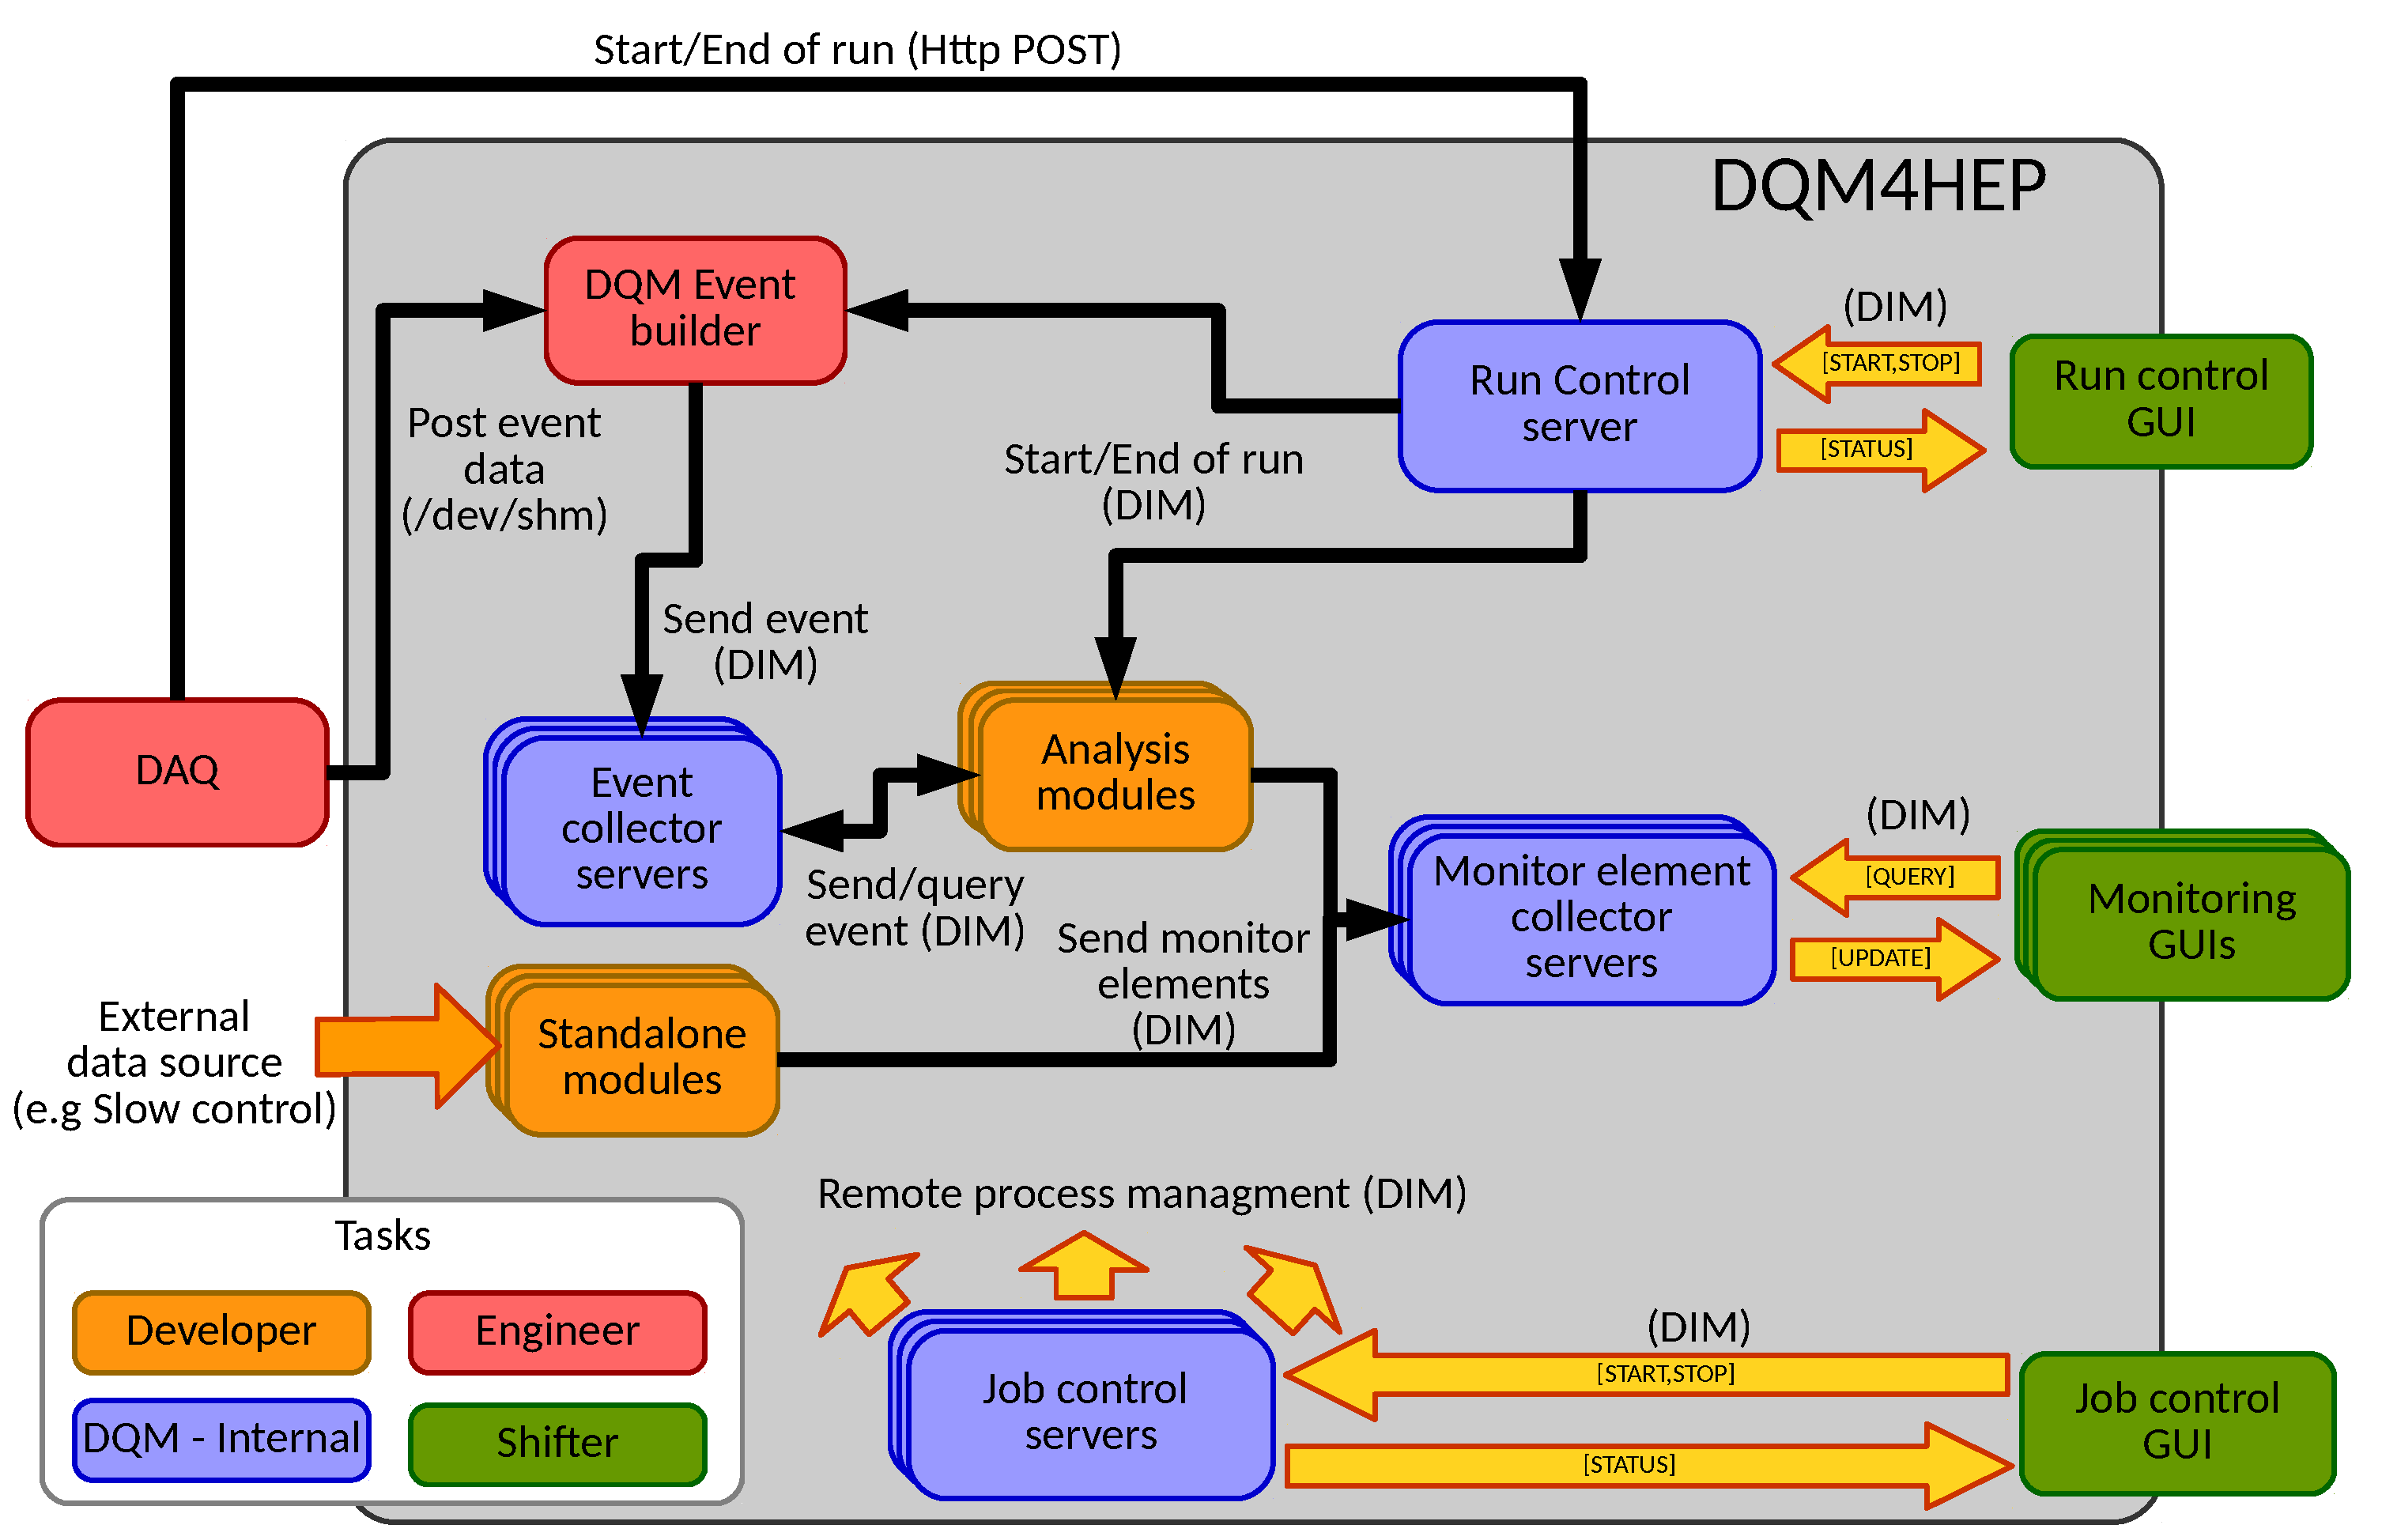
\includegraphics[width=0.95\textwidth]{../Pictures/GlobalArchitectureDiagram.pdf}
	\caption{The global online architecture of \acrshort{DQM4hep}. Each block is colour-coded to show which operator of the testbeam is responsible for the process.}
	\label{figure:daq/dqm4hep/architecture}
\end{figure}

\begin{figure}[p]
	\centering
	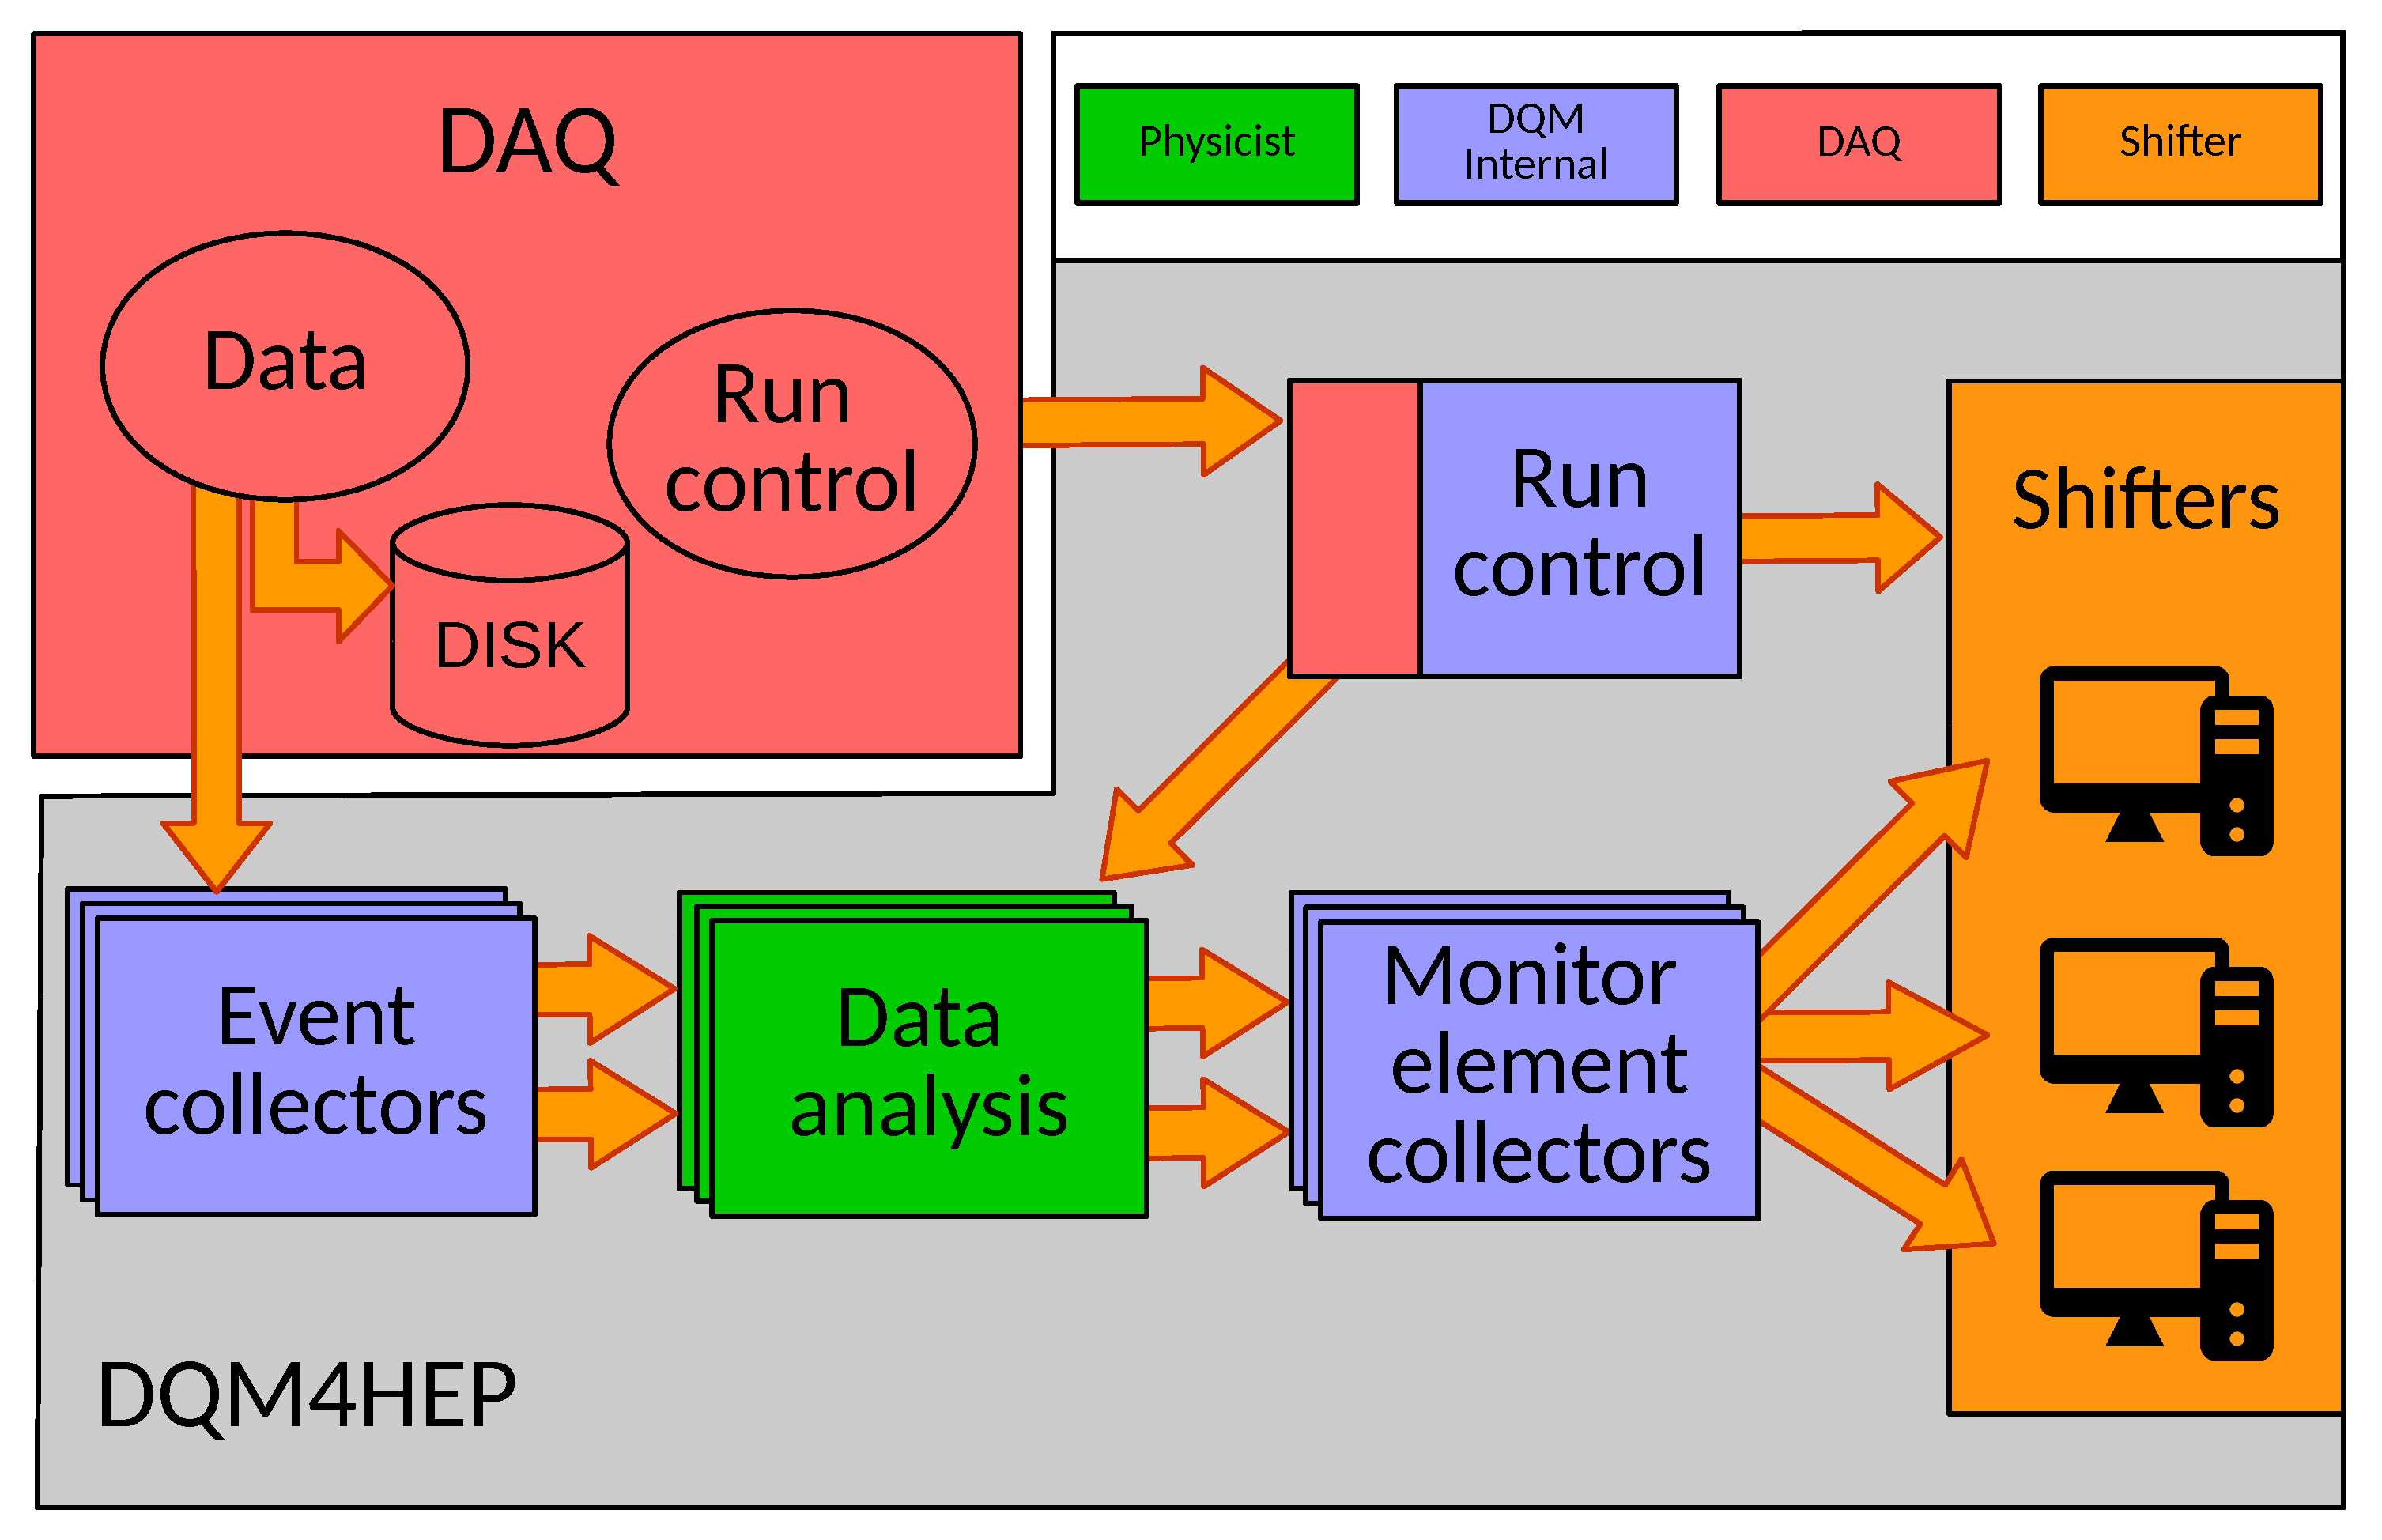
\includegraphics[width=0.95\textwidth]{../Pictures/AnalysisModuleArchitecture.pdf}
	\caption{The structure of running \acrshort{DQM4hep} online using an analysis module.}
	\label{figure:daq/dqm4hep/analysis-module}
\end{figure}

\subsubsection{Analysis modules}
Analysis modules receive events from the data acquisition system, processing the data according to a user-specified procedure to create ROOT TObjects like histograms, graphs, plots, etc. The analysis module then handles encapsulating these objects as monitor elements, and sending them to the rest of the framework for display and storage. 

An analysis module is specific to one use case, and is intended to be written by the user with their data format and processing needs in mind. However, the framework provides both templates and examples for how to write an analysis module. 

An example of the structure of the framework utilising an analysis module can be seen in Fig. \ref{figure:daq/dqm4hep/analysis-module}.

\subsubsection{Standalone modules}
Standalone modules are identical in form to analysis modules described above. The distinction is that a standalone module does not operate on data coming from the data acquisition device. One of the intended and most common usages of standalone modules is as a slow control, taking data from monitoring sensors on the device rather than data, to report on the condition of the hardware. Standalone modules could also be used to \emph{generate} data, if needed, acting as a programmed signal generator or random number generator. 

An example of the structure of the framework utilising a standalone module can be seen in Fig. \ref{figure:daq/dqm4hep/standalone-module}.

\subsubsection{File reader plugins}
A file reader is a type of plugin that reads a file from the disk and packs it into a data structure necessary for usage within \acrshort{DQM4hep}. They are used primarily for offline monitoring or data processing. File readers can be made for any kind of file, provided the user understands the data structure. There are existing examples of file readers for data stored as binary, plain text, \acrshort{LCIO} files, and ROOT TTrees. 

An example of the structure of the framework utilising a file reader plugin can be seen in Fig. \ref{figure:daq/dqm4hep/file-reader}.

\begin{figure}[p]
	\centering
	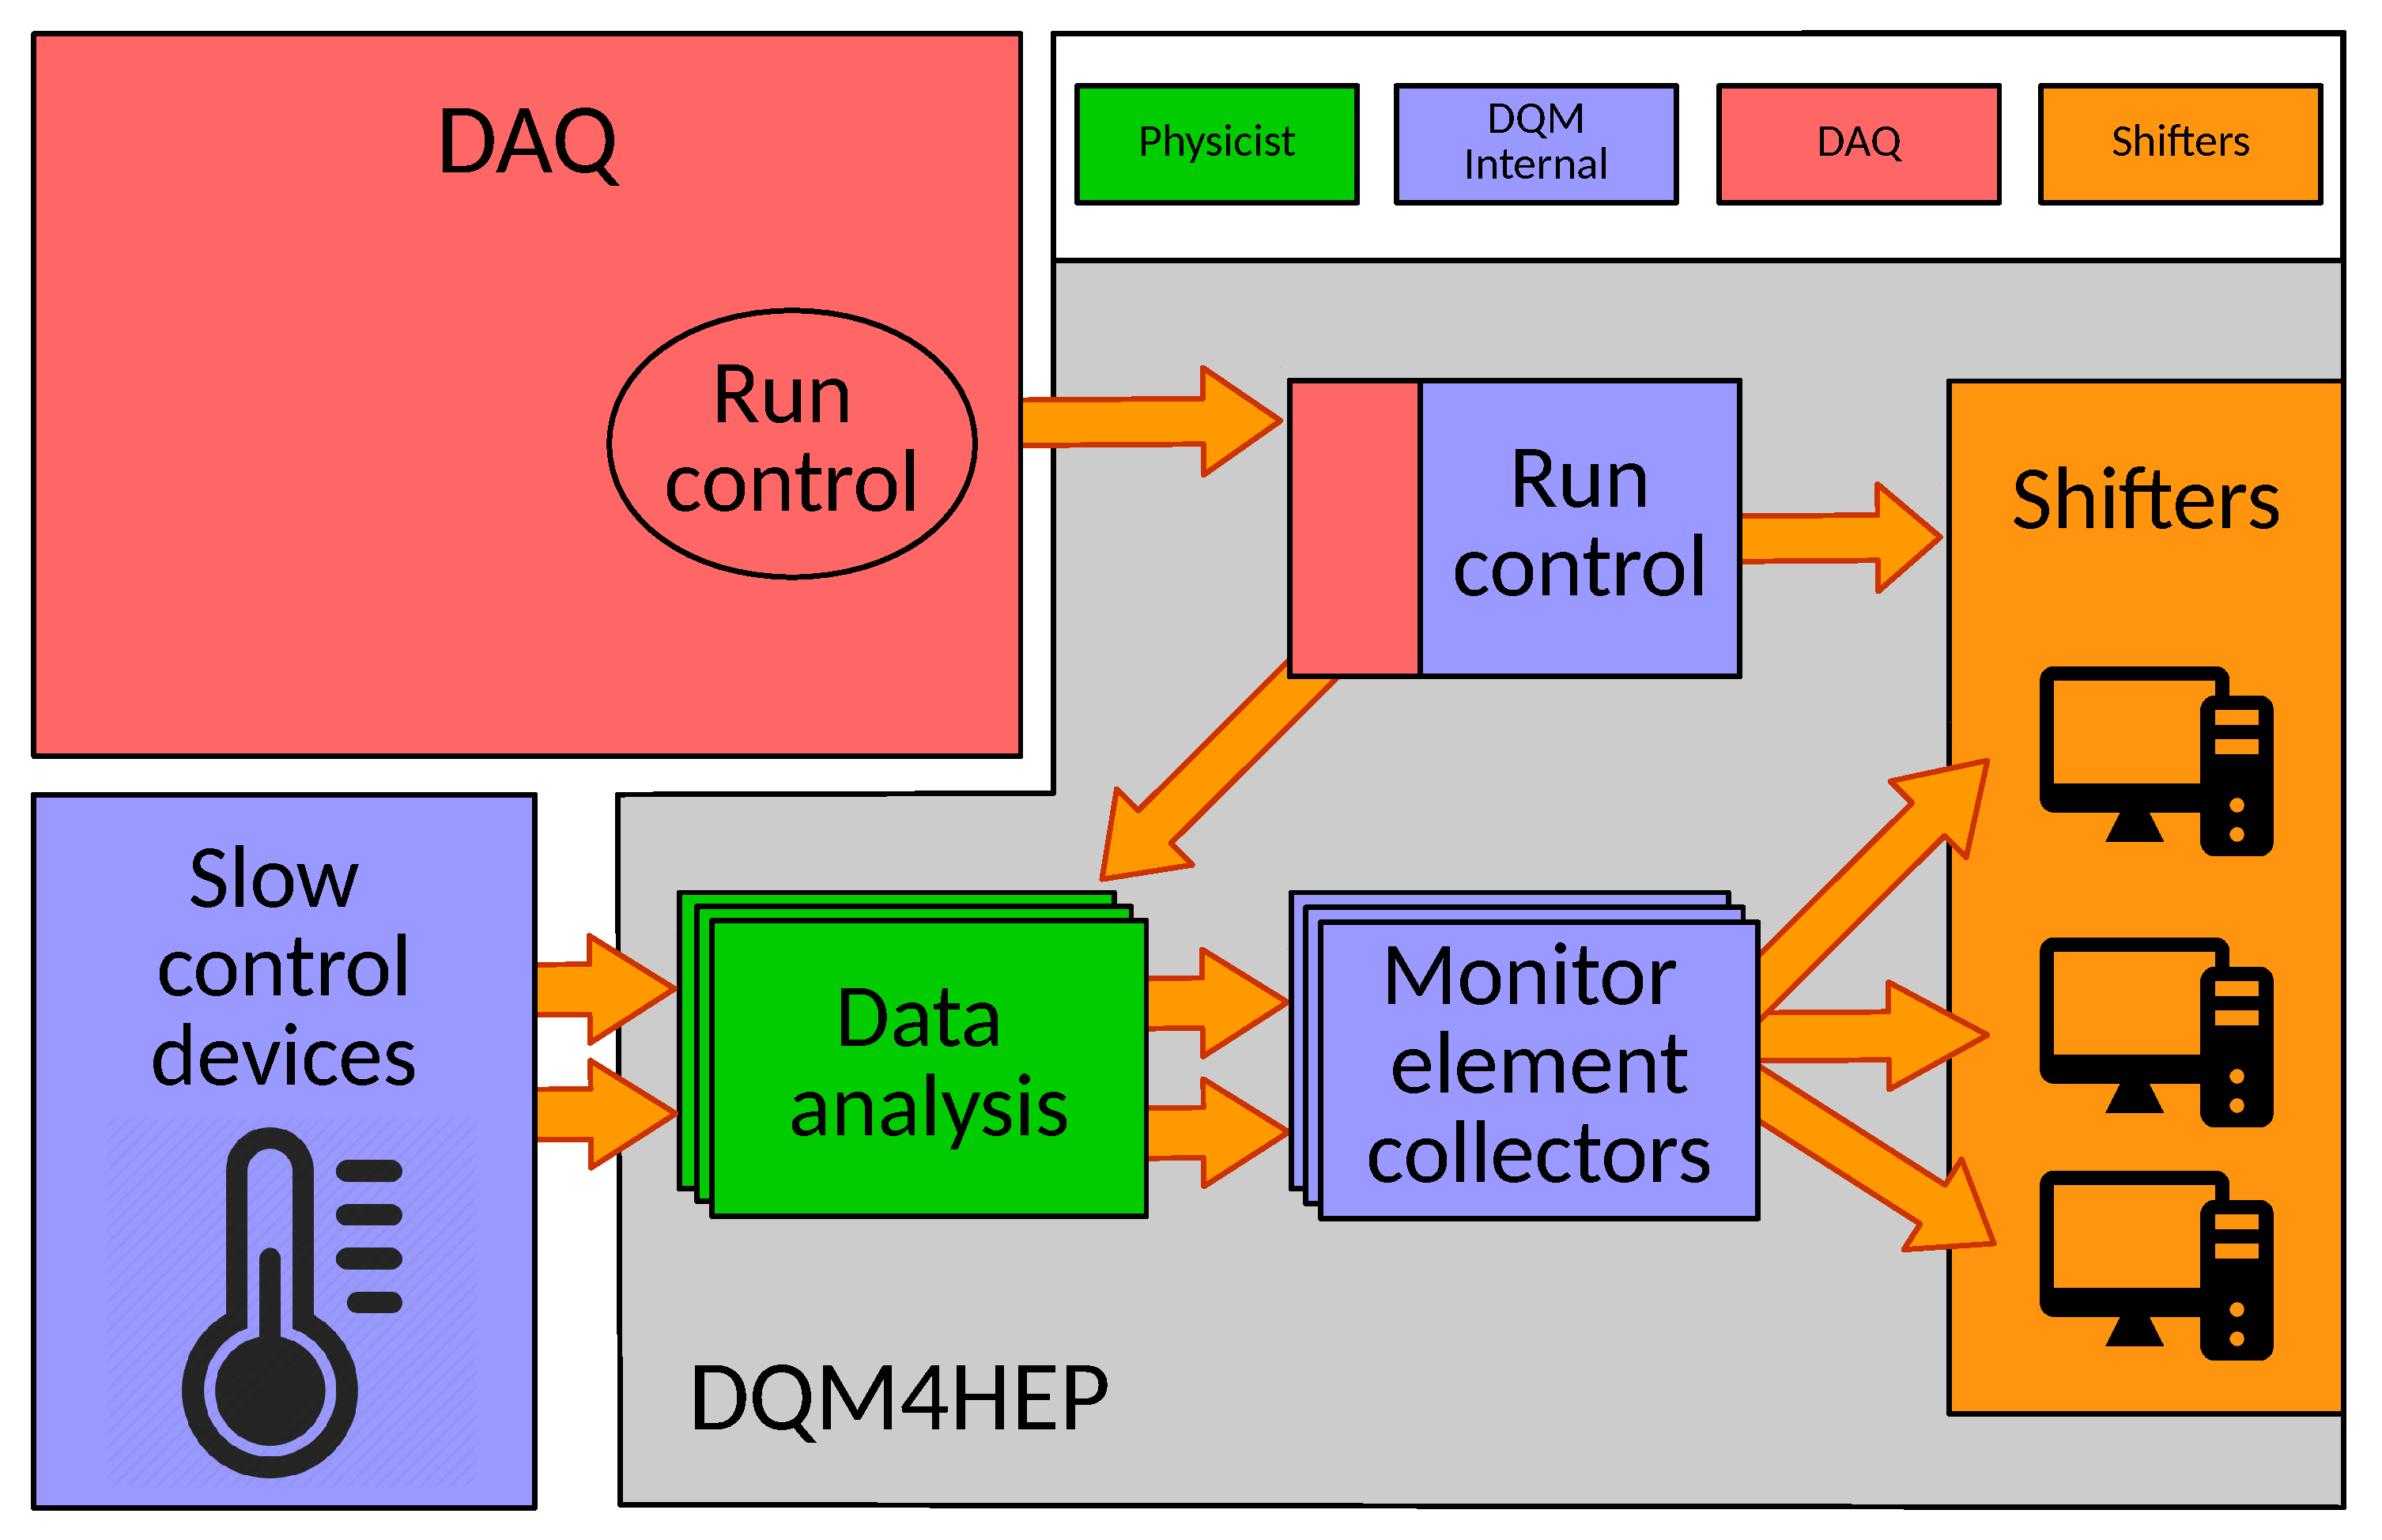
\includegraphics[width=0.95\textwidth]{../Pictures/StandaloneModuleArchitecture.pdf}
	\caption{The structure of running \acrshort{DQM4hep} online using a stand alone module.}
	\label{figure:daq/dqm4hep/standalone-module}
\end{figure}

\begin{figure}[p]
	\centering
	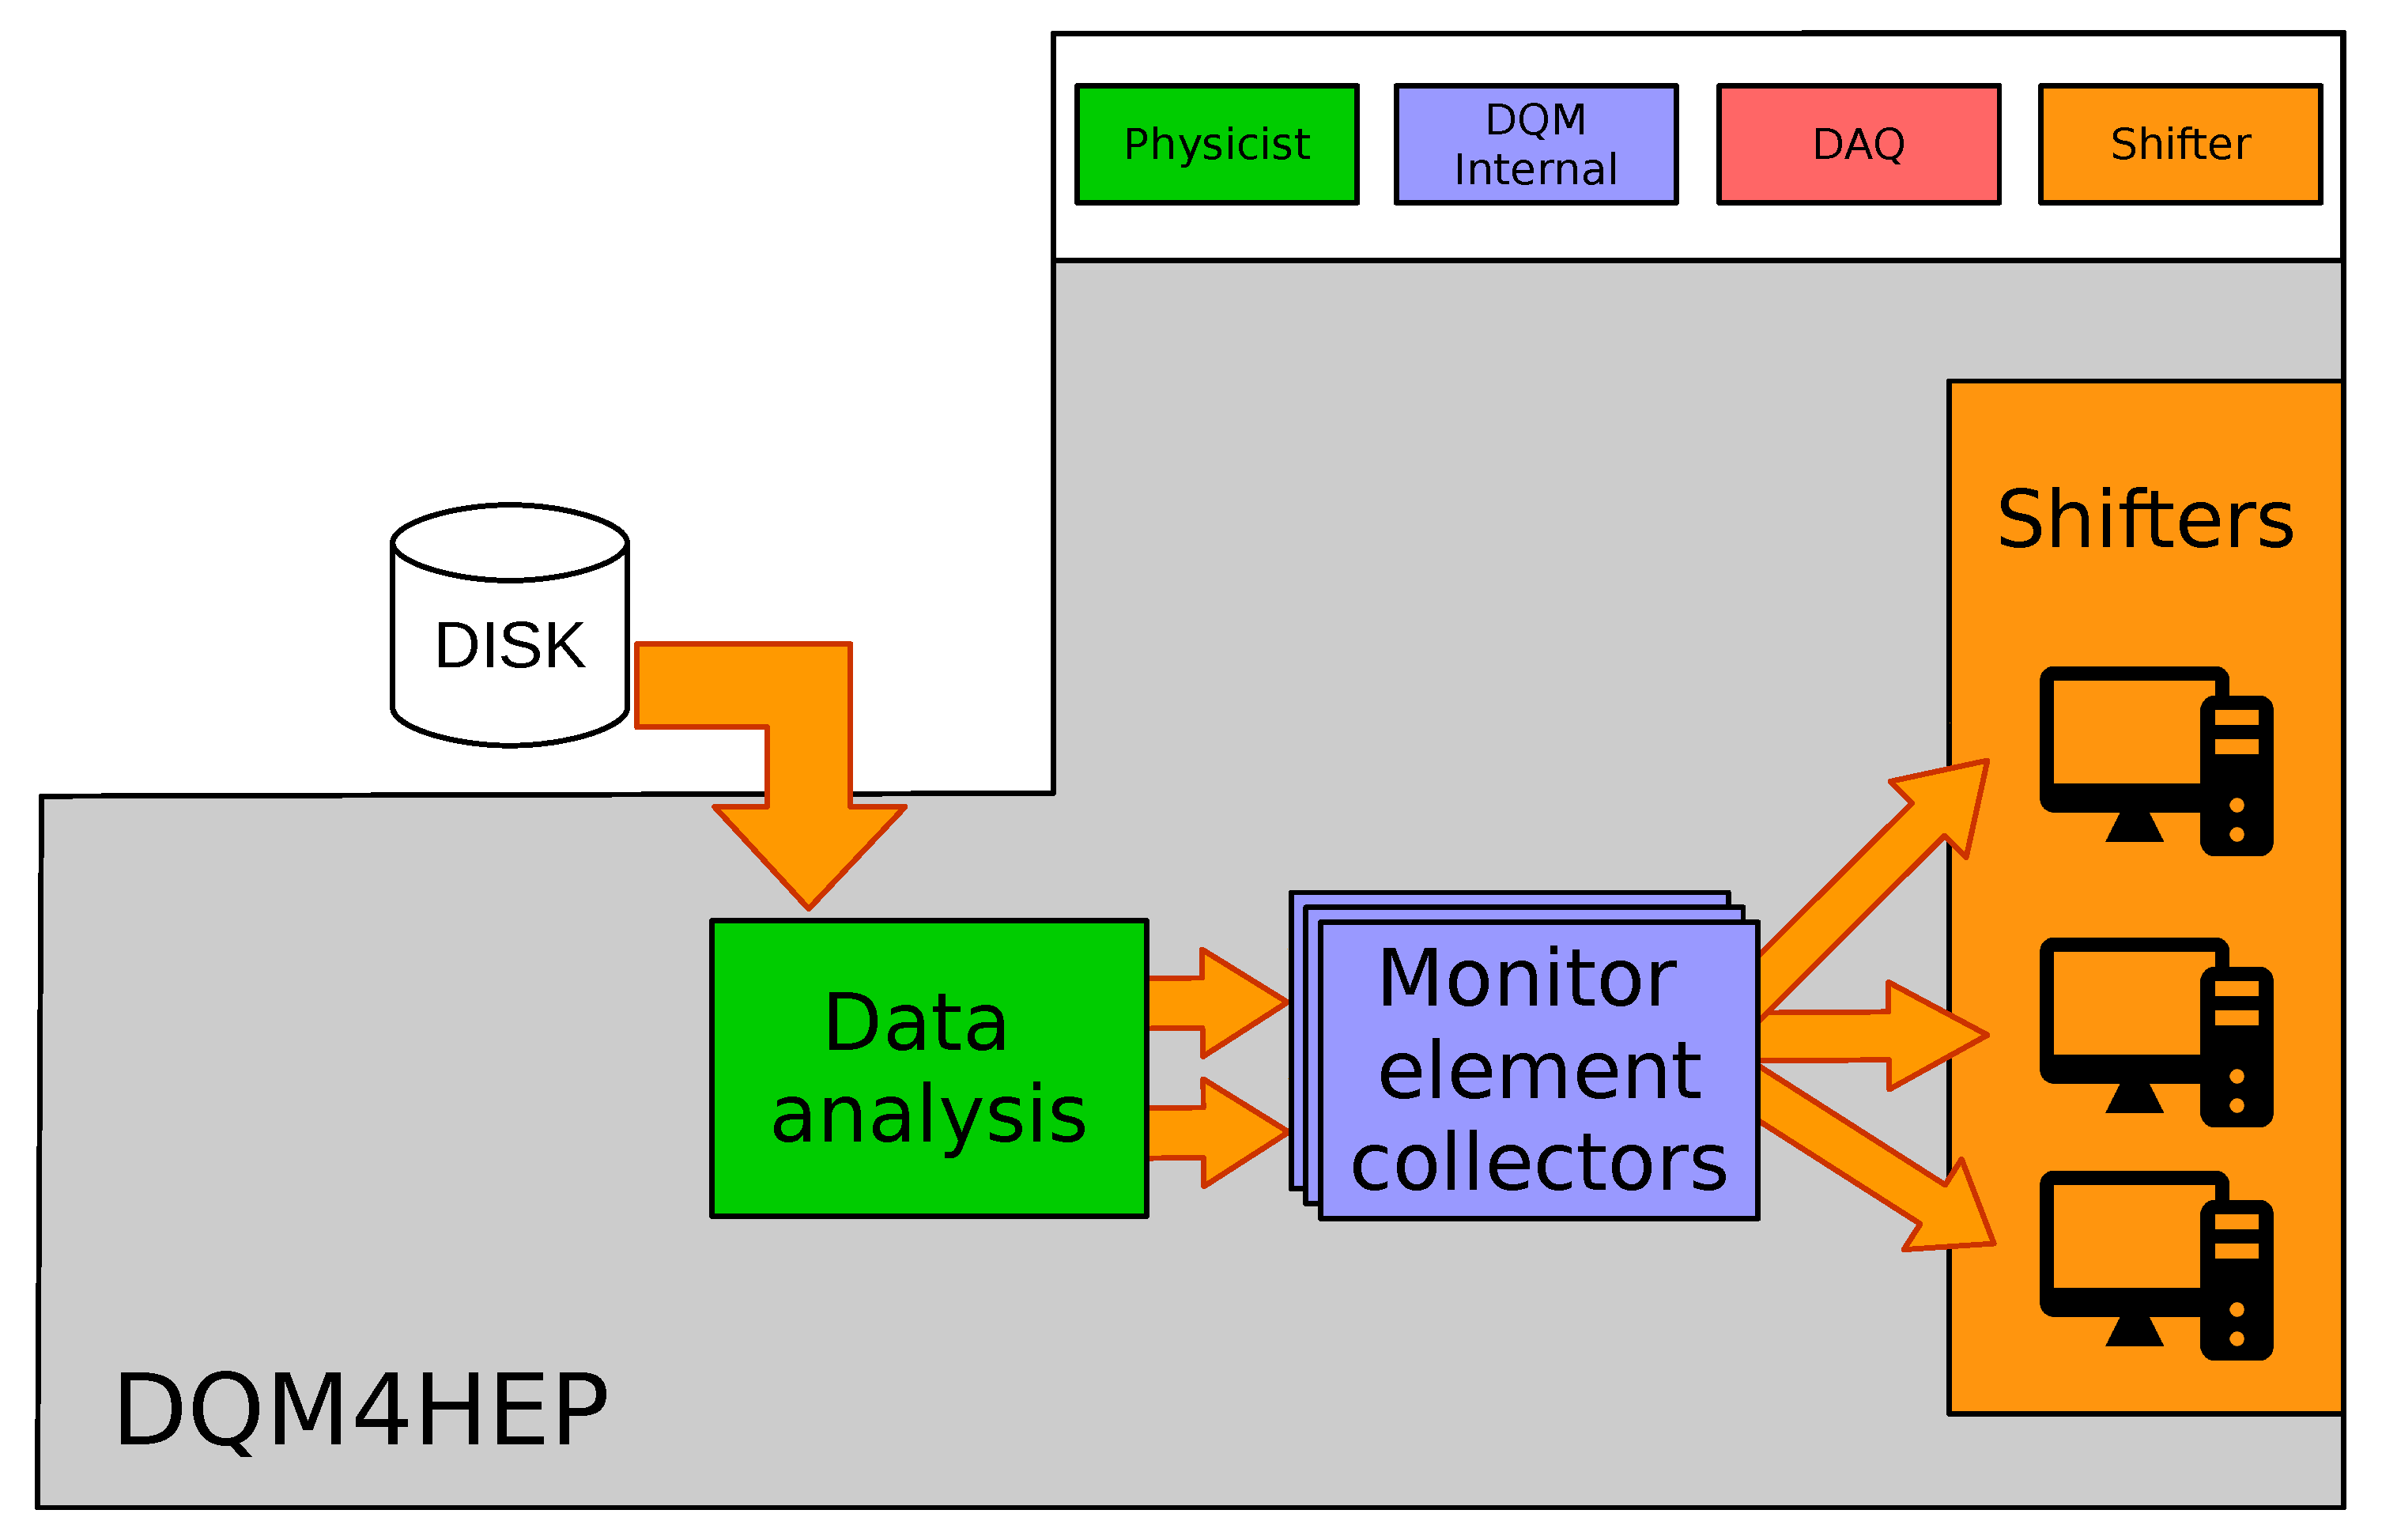
\includegraphics[width=0.95\textwidth]{../Pictures/FileReaderModuleArchitecture.pdf}
	\caption{The structure of running \acrshort{DQM4hep} offline using a file reader module.}
	\label{figure:daq/dqm4hep/file-reader}
\end{figure}

\subsubsection{File streamer plugins}
A file streamer is a type of plugin that reads data from a stream and packs it into a data structure necessary for usage within \acrshort{DQM4hep}. They are for receiving data from a data acquisition device for online monitoring. File streamers can be made for any kind of data stream, provided the user understands the data structure. File streamers are considered the ``default'' in \acrshort{DQM4hep}.

\subsection{Visualisation and graphical user interface}
As of writing, the graphic user interface (\acrshort{GUI}) and visualisation elements of the framework are still under active development for a new version. Therefore this topic will be split into two sections: one to describe the existing \acrshort{GUI}, and one to discuss the motivations and goals for the new \acrshort{GUI} under development. 

\subsubsection{Current GUI and visualisation} 
The current version of the \acrshort{GUI} is built with Qt, a free and open-source toolkit and framework for creating graphic user interfaces and widgets that are independent of the operating system. The motivation for choosing Qt was that ROOT provides an option for integration between ROOT and Qt, allowing ROOT classes like \texttt{TCanvas} to be ``embedded'' into Qt widgets. This simplified the implementation of a \acrshort{GUI}, allowing a graphical interface based on Qt to be written, then graphics from ROOT simply opened within the existing widgets and windows. % We should cite this; this information is from here: (https://root.cern.ch/root/html534/guides/users-guide/ROOTandQt.html). 

This interface is used in multiple places, including the run control process and the monitoring \acrshort{GUI}. The monitoring \acrshort{GUI} is built on a system of canvases. Each canvas can have multiple plots open, which can be resized, maximised, minimised, etc. and manipulated as normal for ROOT plots. The user can also create new canvases for more space to arrange plots.

In addition to this, there is an optional provision for a monitoring steering file, which contains presets of canvases, and the plots displayed on them. This is extremely useful when dealing with large datasets or large numbers of plots, as the plots required by the user can be opened automatically when the monitoring interface is run.

An example of the Qt-based monitoring \acrshort{GUI} in use can 3be seen in Fig. \ref{figure:daq/dqm4hep/old-gui}. 

\begin{figure}[h]
	\centering
	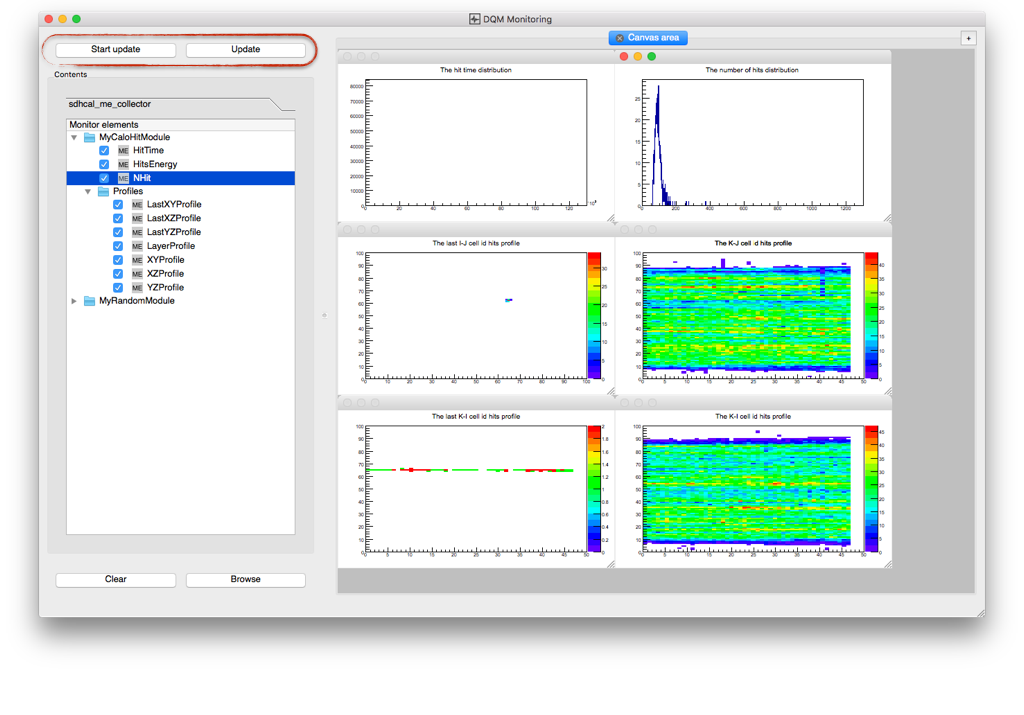
\includegraphics[width=1.0\textwidth]{../Pictures/DQM4hepMonitoringGui.png}
	\caption{An example of the current Qt-based monitoring \acrshort{GUI} in use.}
	\label{figure:daq/dqm4hep/old-gui}
\end{figure}

\subsubsection{New user interface and visualisation package}
For the newer versions of \acrshort{DQM4hep}, the decision was made to overhaul the \acrshort{GUI} and visualisation packages, removing Qt from the framework and moving to a web-based interface.

The removal of Qt was motivated by two reasons. Firstly, the integration with ROOT provided some complications, since running \acrshort{DQM4hep}'s Qt-based \acrshort{GUI} requires an installation of ROOT compiled with the \texttt{--enable-Qt} flag enabled. The majority of ROOT installations in remotely-accesible file systems based at \acrshort{CERN} and \acrshort{DESY} (which are heavily used for analysis and testbeams) were not compiled this way. Secondly, Qt was an additional dependency that must be installed prior to use, making the software more dependent upon the operating system, compiler tools, and environment of the machine, and thus less generic and easy to use. % Also isn't Qt support getting removed from ROOT soon? We'd need a citation for that though.

The removal of the Qt \acrshort{GUI} allows for greater freedom with development. The intended goal is to have a browser-based GUI, removing dependency on any external \acrshort{GUI} libraries and allowing it to function on any device. This will also make it more user-friendly and convenient, as the interfaces for run control, networking, and data monitoring and quality display can be simply run in different tabs of a web browser.

As of writing, the web interface is under active development by R\'{e}mi Et\'{e} and is not yet complete. However, a mock-up of the web interface can be seen in Fig. \ref{figure:daq/dqm4hep/future-gui}.

\begin{figure}[h]
	\centering
	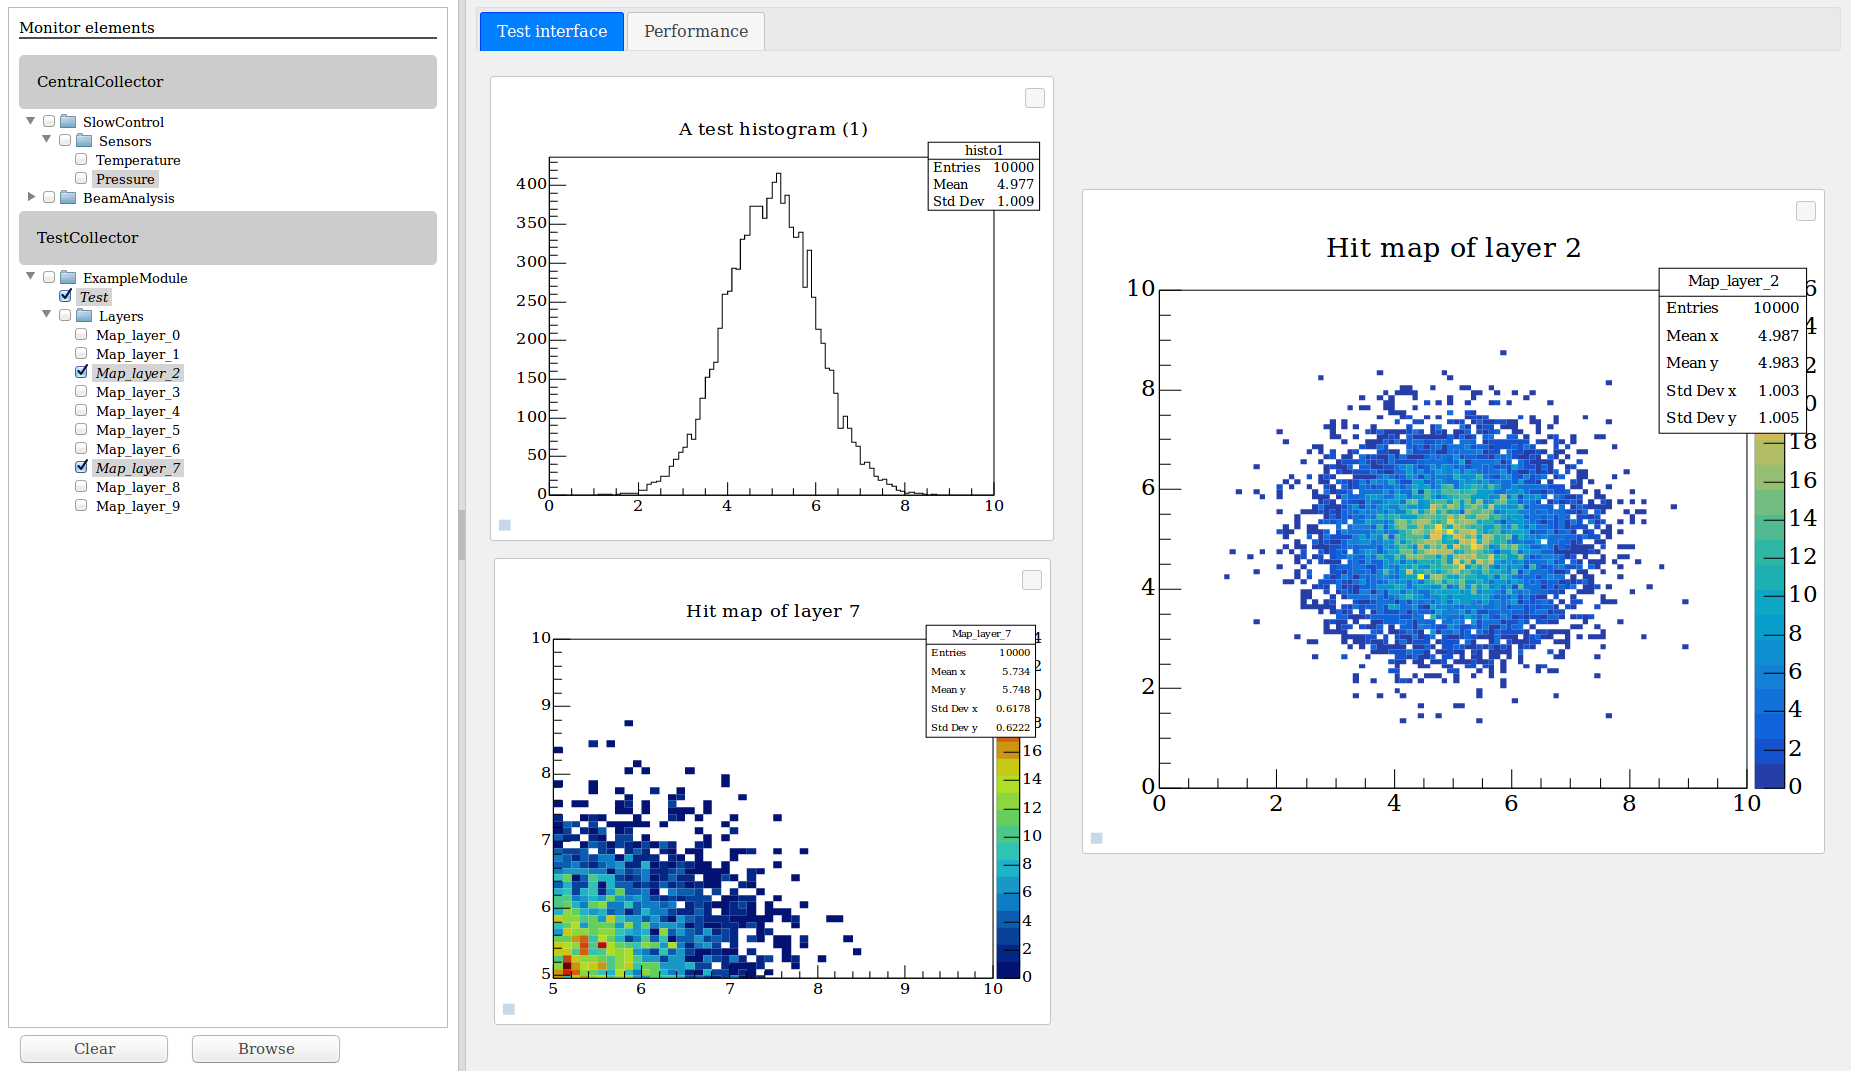
\includegraphics[width=1.0\textwidth]{../Pictures/ScreenshotWebMonitoring.png}
	\caption{A preview of the planned web-based monitoring interface.}
	\label{figure:daq/dqm4hep/future-gui}
\end{figure}

\section{Analysis modules}
An analysis module is a plugin that uses data to create monitor elements, which are the core object that drives online monitoring in \acrshort{DQM4hep}. Analysis modules are thus a central piece of using \acrshort{DQM4hep} as an online monitor.

Mechanically, analysis modules are plugins that read events from a file reader or file streamer plugin, perform some user-defined process to the data to produce a plot, graph, histogram or other ROOT object before emitting it to the rest of the framework as a monitor element.

The most basic analysis module will simply structure information coming from the data acquisition device into a human-readable plot, but analysis modules are able to do anything that can be done in C++ or ROOT, so can contain an arbitrary amount of processing. This means that analysis modules can also be used for online analysis or processing of data, making them very powerful tools for online monitoring. 

\subsection{Running an analysis module}
The \texttt{dqm4hep-start-module} executable is used to run an analysis module, in combination with an XML steering file. The available arguments are as follows:

\begin{lstlisting}
-h
--help
\end{lstlisting}

Displays usage information, then exits.

\begin{lstlisting}
-f
--steering-file
\end{lstlisting}

(Required) Gives the path to the XML steering file that defines what analysis modules to run and their parameters. See the section below (need link) for more information on these steering files. 

\begin{lstlisting}
-t
--type
\end{lstlisting}

The type of module to run. This overwrites the module type in the steering file.

\begin{lstlisting}
-n
--name
\end{lstlisting}

The name for this instance of the module. This overwrites the module name in the steering file.

\begin{lstlisting}
-v
--verbosity
\end{lstlisting}

The verbosity of the logger. Options are \texttt{trace}, \texttt{debug}, \texttt{info}, \texttt{warning}, \texttt{error}, \texttt{critical}, and \texttt{off}. This is \texttt{warning} by default.

\begin{lstlisting}
--
--ignore-rest
\end{lstlisting}

Ignores any arguments following this flag.

\begin{lstlisting}
--version
\end{lstlisting}

Displays version information, then exits.

\subsubsection{Steering files}
An \acrshort{XML} steering file is used to pass parameters to the analysis module, including the type of analysis module, the plots to create, and what other processes to connect to. An example steering file can be found in the \texttt{dqm4hep-example/tests/} directory.

Steering files are broadly made of four sections: the application settings, the archiver settings, the analysis module, and the monitor elements.

The application settings specify how to run the application itself, including which other file readers or streamers to connect to, which run control is being used, etc. 

The archiver setting specify whether the results of running the analysis module are written to an archive, which is a ROOT file containing the monitor elements that the analysis module created.

The analysis module section sets the type of analysis module to run, and gives it a unique name to distinguish it from other instances of the same module. Both of these parameters can be set at the command line (see above).

The monitor element section specifies the monitor elements used in the file. Monitor elements is a general name for any kind of ROOT object, which may be a histogram, graph, plot, drawing, etc. The name, directory, and properties of monitor elements are set here, depending on what type of object the monitor element is.

\subsection{Creating analysis modules}
The \acrshort{DQM4hep} pages on Github have a repository to accompany this documentation – the \texttt{dqm4hep-example} package is available here\refthis. This package contains all of the tools necessary to immediately begin writing and compiling analysis modules for an existing installation of \acrshort{DQM4hep}. 

It is recommended to fork this repository before starting, so git and Github's version control features can be used to back up code.

In addition to writing the analysis module code, a compiled analysis module needs to be declared as a plugin for \acrshort{DQM4hep} to be able to use it. The absolute path to the library file for new analysis modules needs to be appended to the \texttt{DQM4hep\textunderscore PLUGIN\textunderscore DLL} environment variable. 

\subsubsection{Writing analysis modules}
Analysis modules must be written specifically for the type of data they recieve and for a certain analysis or set of analyses to perform. This means that the ideal person to write an analysis module is someone familiar with both the experiment's event structure and the goals of the monitoring.

Each analysis module is a single .cc file. E.g. \texttt{ExampleModule.cc} defines an analysis module called \textit{ExampleModule} that can be found in the \texttt{dqm4hep-example/source/src/plugins} directory.

The .cc file then has several sections that must be written, described in separate sections below.

\subsubsection{Variable declaration}
In this section of the file, the variables that must be persistent over the entire running of the module are declared. These variables will not go out of scope, so are usually reserved for the monitor elements themselves, or counters that must persist over the entire module. Monitor elements must be declared as the \texttt{online::OnlineElementPtr} type. None of the declared variables are initialised here; initialision is done in later functions.

\subsubsection{readsettings}
This function reads the settings from the XML steering file, meaning that anything that needs to be initialised from the steering file is done here. This notably includes all monitor elements. Typically the \texttt{core::OnlineElementPtr} will have been declared during the (preamble), then is assigned here based on the steering file using the \texttt{online::ModuleApi::getMonitorElement()} function. 

\subsubsection{initModule}
This process is run once, when the analysis module is initialised. Anything that needs to be done only once at the beginning should be done here. The use of this function is limited, as most tasks that need to be reset are reset at the beginning of a run using \texttt{startOfRun()} below.

\subsubsection{startOfRun}
The \texttt{startOfRun} function handles code that should be executed only once per run, at the beginning. This is commonly used for counters that must persist over the entire run, for instance if a detector can give an error signal, a counter to store the number of error signals is initialised here so that it is persistent over the entire run, and the number of error signals can be totalled at the end of the run.

%\subsubsection{startOfCycle}

%\subsubsection{endOfCycle}

\subsubsection{endOfRun}
This is the end-of-run counterpart to \texttt{startOfRun()}. In general, this function will encapsulate logic that must deal with counters or procedures that were intialised or begun in \texttt{startOfRun()}.

\subsubsection{endModule}
This function is called when the module ends, and is usually used for deleting or cleaning up any objects created during the \texttt{initModule()} function. Most normal use cases will not need this function, as cleanup of objects such as variables or monitor elements is handled by the framework.

\subsubsection{process}
This is the function where the analysis module performs the main processing of data. In this function, events are loaded into memory from the event stream or file reader, and made available for use. Data can then be processed using normal C++ methods, then filled into monitor elements to be sent to the monitor element collectors so they can be presented in the user interface, or stored by the archiver.

\subsubsection{Plugin declaration}
Analysis modules are \acrshort{DQM4hep} plugins, so must be declared as a plugin using \acrshort{DQM4hep}'s facility for this so that the main executables can access them. At the end of the module, the following code must be included to declare the analysis module as a plugin:

\begin{lstlisting}
DQM_PLUGIN_DECL(ModuleName, "ModuleName");
\end{lstlisting}

This should take place at the very end of the file but within the \texttt{dqm4hep} and \texttt{example} namespaces.

When an analysis module is declared as a plugin, the main \acrshort{DQM4hep} executable must be given the directory of the library to load the plugin at runtime. This is done by appending the director of the library to the \texttt{DQM4hep\textunderscore PLUGIN\textunderscore DLL} environment variable:

\begin{lstlisting}
export DQM4hep_PLUGIN_DLL=$DQM4hep_PLUGIN_DLL:/path/to/module/lib/libDQMExample.so
\end{lstlisting}

Once this is added, \acrshort{DQM4hep} can access the libraries and run the analysis module.

\subsection{SimpleModule – a worked example} 
To explain the process of creating and writing analysis modules in more detail, a worked example is presented. For this we imagine a simplified particle physics detector, and write an analysis module called \texttt{SimpleModule.cc} to monitor data from it. We also write a steering file called \texttt{simple-test.xml} to run the analysis module. Each function of the analysis module will be described in depth, explaining in detail what the code is doing. 

In this example, the built-in GenericEvent event type is used. For more information on the GenericEvent type, see\refthis . We will not be using the \texttt{startOfCycle} and \texttt{endOfCycle} functions.

The full version of these files can be found in the dqm4hep-example repository, available here \refthis .

\subsubsection{Detector}
We can imagine a simplified particle physics detector as a square plane split into 36 tiles (6 on each side). When a hit occurs the detector reads out the location, \acrshort{ADC}, and time of the hit. Each event will correspond to a single hit.

The data acquisition device sends us an event made of four integer values:

\begin{itemize}
	\item xPos -- the position of a hit on the x-axis of the detector, from 0 to 5
	\item yPos -- the position of a hit on the y-axis of the detector, from 0 to 5
	\item ADC -- the \acrshort{ADC} of the hit, in arbitrary units, between 0 and 1500
	\item timeHit -- the time the hit occured, in arbitrary units
\end{itemize}

\subsubsection{Goals}
Before writing the module, the variables and properties to monitor must be determined. For this detector and its analysis module, there are three goals:

\begin{itemize}
	\item Spectrum histogram -- a single histogram containing the \acrshort{ADC} of each hit for the entire run, producing an energy spectrum.
	\item Hitmap -- a hitmap showing the distribution of hits across the detector.
	\item Radiation damage -- if we imagine that \acrshort{ADC}s higher than 1000 are likely to cause radiation damage to the detector, then monitoring the number of hits in the entire run exceeding this threshold allows an estimation of how damaged the detector may be.
\end{itemize}

\subsubsection{Preamble}
Here the pointers for all monitor elements are initialised. One is required for the \acrshort{ADC} spectrum, and one for the hitmap. They don't need to have their type declared here -- this is done later. The standard style for \acrshort{DQM4hep} is to prefix all monitor element pointers with \texttt{m\textunderscore p} to distinguish them, as they are an important type.

Variables for handling the information about radiation damage are also created here, as they need to persist between events. These are declared here and will be initialised later.

\begin{lstlisting}
private:
  online::OnlineElementPtr m_pSpectrum;
  online::OnlineElementPtr m_pHitmap;
  int radiationDamageADCThreshold;
  int damageHitsCounter;
\end{lstlisting}

\subsubsection{readSettings}
Here the monitor elements are assigned, reading in their information from the \acrshort{XML} steering file. To do this the \texttt{online::ModuleApi::getMonitorElement()} function is used, which searches in the \acrshort{XML} steering file for the corresponding information. This function has three arguments: the first is always \texttt{this}, the second is the directory the monitor element is in, and the third is a string of the name given to the monitor element in the steering file. These monitor elements are placed at the top directory, so the second argument is \texttt{/}.

\begin{lstlisting}
void SimpleModule::initModule() {
  m_pSpectrum = online:ModuleApi::getMonitorElement(this, "/", "ADC_Spectrum");
  m_pHitmap   = online:ModuleApi::getMonitorElement(this, "/", "Hitmap");
}
\end{lstlisting}

Any other variables that need to be initialised only when the module starts should be placed here. This is a good place to define the threshold for radiation damage:

\begin{lstlisting}
  radiationDamageADCThreshold = 1000;
\end{lstlisting}

\subsubsection{startOfRun}
The only thing necessary to do at the start of each new run is to ensure that the counter for hits above the threshold for radiation damage is reset to zero:

\begin{lstlisting}
void SimpleModule::startOfRun(core::Run &/*run*/) {
    damageHitsCounter = 0;
}
\end{lstlisting}

This ensures that even with multiple runs in the same file, the counter resets correctly.

\subsubsection{endOfRun}
Once a run has finished, the number of hits that might have caused radiation damage should be read out. There are many ways to do this, but the simplest is to send a message to the logger:

\begin{lstlisting}
void SimpleModule::endOfRun(const core::Run &/*run*/) {
    dqm_info("Number of hits above radiation damage threshold: {0}", damageHitsCounter);
}
\end{lstlisting}

For more information on the \texttt{dqm \textunderscore info()} function and it's syntax, see the section on the logging tools here \refthis .

\subsubsection{process}
The first thing to do is make sure that the \texttt{process()} function has access to the GenericEvent. This is done by making it an argument of the function, calling it \texttt{pEvent} to make it clear that this is a pointer to an event and not an event object. Basic error-checking is then done, to ensure that the current event exists:

\begin{lstlisting}
void SimpleModule::process(core::EventPtr pEvent) {

  if (nullptr == pEvent) {
    dqm_warning("Event pointer is invalid - skipping this event");
    return;
  }
\end{lstlisting}

The \texttt{dqm\textunderscore warning()} function publishes a message to the logger, with the \texttt{warning} level. See the section on the logging tools for more information \refthis .

Forcing this function to \texttt{return} ensures that the an analysis module doesn't attempt to access an event that does not exist. Otherwise, this would cause a segmentation fault and crash the analysis module. Since the \texttt{process()} function runs separately for each event, this has the effect of skipping to the next event.

Now the pointer of the event needs to be assigned so that the object itself can be accessed. A new variable of type \texttt{core::GenericEvent} is created, then the \texttt{getEvent()} function is used to assign it.

\begin{lstlisting}
  core::GenericEvent *pGenericEvent = pEvent->getEvent<core::GenericEvent>();
\end{lstlisting}

A variable is needed to store the information pulled from the event, then the information can be extracted using the \texttt{getValues()} function:

\begin{lstlisting}
  int xPos;
  int yPos;
  int ADC;
  int timeHit;

  pGenericEvent->getValues("xPos", xPos);
  pGenericEvent->getValues("yPos", yPos);
  pGenericEvent->getValues("ADC", ADC);
  pGenericEvent->getValues("timeHit", timeHit);
\end{lstlisting}

The \texttt{getValues()} function takes two arguments: the first is a key in the form of a string, which identifies a piece of data within the GenericEvent. The second is the object to place the retrieved data into. In this case, the same names are used for simplicity. This works because the first variable is a string, used as a key to find information within the GenericEvent.

Now all the data is loaded into memory and available for use. 

First the ADC is added to the \texttt{ADC\textunderscore Spectrum} plot. To do this, the monitor element \texttt{m\textunderscore pSpectrum} must be cast to the correct ROOT object type, using the \texttt{objectTo()} function, then use ROOT's \texttt{Fill()} function:

\begin{lstlisting}
  m_pSpectrum->objectTo<TH1I>()->Fill(ADC);
\end{lstlisting}

Then the same must be done for the hitmap. This time it needs to be cast to a TH2I object and filled with the x- and y-positions as well as the \acrshort{ADC}:

\begin{lstlisting}
  m_pHitmap->objectTo<TH2I>()->Fill(xPos, yPos, ADC);
\end{lstlisting}

And lastly, a check is performed for whether the \acrshort{ADC} was high enough to cause radiation damage, and if so increment the counter:

\begin{lstlisting}
  if (ADC >= radiationDamageADCThreshold) {
    damageHitsCounter++;
  }
\end{lstlisting}

\subsubsection{Steering file}
Now the analysis module is complete, there needs to be a steering file to run it. This is started by making a file called \texttt{simple-test.xml}. Then the \texttt{<dqm4hep>} environment is opened, as this will contain everything else:

\begin{lstlisting}
<dqm4hep>

    <!-- everything else will be in here -->

</dqm4hep>
\end{lstlisting}

There are then four sections to write: the application settings, the archiver settings, the analysis module, and the monitor elements.

\subsubsection{Application settings}
This section of the steering file controls the parameters that are needed to run the module itself. This part of the file is where the module is specified to be running online (receiving events from an event collector) or offline (receiving events from a file reader).

This analysis module will be run offline, so the important fields here are \texttt{EventReader}, which is which type of file reader to use to read events, and \texttt{EventFileName}, which specifies the path to the file to read.

If this were running online, the \texttt{RunControl}, \texttt{EventCollector}, \texttt{EventSource} and \texttt{MonitorElementCollector} would have to give the names of those processes. When running offline, these names can be set to anything, so they are given dummy names.

\begin{lstlisting}
<settings mode="EventReader">
  <parameter name="EnableStatistics"> true </parameter>
  <parameter name="EventReader"> SimpleEventReader </parameter>
  <parameter name="EventFileName"> /foo/bar/simpleEventDatafile.root </parameter>
  <parameter name="CyclePeriod"> 1 </parameter>
  <parameter name="CycleCounter"> 0 </parameter>
  <parameter name="CycleTimeout"> 0 </parameter>
  <parameter name="RunControl"> DummyRunControl </parameter>
  <parameter name="EventCollector"> DummyEventCollector </parameter>
  <parameter name="EventSource"> DummyEventSource </parameter>
  <parameter name="MonitorElementCollector"> DummyMECollector </parameter>
</settings>
\end{lstlisting}

\subsubsection{Archiver settings}
This section controls the archiver, which creates an archive of all monitor elements in the form of a ROOT file when the analysis module exits. If the archiver isn't needed, it can be set to \texttt{enable="false"} and ignored.

In this case the archiver is needed, so it is set to \texttt{true}. A filename for the archive needs to be given, e.g. \texttt{archive-run42.root}. The OpenMode is chosen to be \texttt{RECREATE} as the archive should be re-written every time the module is run, although \texttt{APPEND} would add events onto an existing file. \texttt{AllowOverwrite} is set to \texttt{true} so that old archives can be overwritten easily. As run numbers are not used in the analysis module, \texttt{AppendRunNumber} is set to \texttt{false}.

\begin{lstlisting}
<archiver enable="true">
  <parameter name="FileName" value="archive-run42.root"/>
  <parameter name="OpenMode" value="RECREATE"/>
  <parameter name="AllowOverwrite" value="true"/>
  <parameter name="AppendRunNumber" value="false"/>
  <selectors>
    <selector regex=".*" select="true"/>
  </selectors>
</archiver>
\end{lstlisting}

\subsubsection{Analysis module}
This section contains a declaration of which analysis module to execute, and the name to give it. A running analysis module needs a unique name to distinguish it from other modules of the same type running in the same environment.

This steering file has to run SimpleModule. Only one instance is needed at a time, but the name has to be different than the module's base name, so:

\begin{lstlisting}
<module type="SimpleModule" name="mySimpleModule"/>
\end{lstlisting}

\subsubsection{Monitor elements}
This section is where the monitor elements to use and the parameters of the ROOT objects are declared. This entire section will be within the \texttt{<storage>} and \texttt{<monitorElements>} environments:

\begin{lstlisting}
<storage>
  <monitorElements>

    <!-- monitor elements will go here -->

  </monitorElements>
</storage>
\end{lstlisting}

To create a ROOT object, the \texttt{<bookElement>} environment is used to declare it's type, path, name, title, and any other parameters the ROOT object requires. For example, to create a histogram for the \acrshort{ADC} spectrum, a TH1I is needed as the \acrshort{ADC}s are integers. The range of the \acrshort{ADC}s is from 0 to 1500, so the range can be set accordingly.

\begin{lstlisting}
<bookElement type="TH1I" path="/" name="ADC_Spectrum" title="Spectrum of all ADCs" nBinsX="150" minX="0" maxX="1500">
</bookElement>
\end{lstlisting}

Similarly, the monitor element for the hitmap is defined:

\begin{lstlisting}
<bookElement type="TH2D" path="/" name="Hitmap" title="Hitmap of the example detector" nBinsX="6" minX="0" maxX="5" nBinsY="6" minY="0" maxY="5">
</bookElement>
\end{lstlisting}

\subsubsection{XML loops}
In this example, loops aren't necessary, but defining monitor elements using a for-loop in \acrshort{XML} is a useful feature, so it is discussed here. For example, if one of the goals were to create a histogram for each of the 36 tiles in the detector, a for-loop would allow thtis to be created with a smaller amount of code

To do this, the \texttt{<for>} environment is used, using \texttt{tileNumber} as the id. Then a template monitor element defintion is written out using \texttt{\$ FOR{tileNumber}} whenever the tile number should be inserted:

\begin{lstlisting}
<for id="tileNumber" begin="0" end="35" increment="1">
  <bookElement type="TH1D" path="/" name="Tile$FOR{channelNum}" title="Spectrum for tile $FOR{channelNum}" nBinsX="150" minX="0" maxX="1500">
  </bookElement>
</for>
\end{lstlisting}

This would then create a series of monitor elements called \texttt{Tile0}, \texttt{Tile1}, \texttt{Tile2}, etc.

\subsubsection{Building and running}
To compile the analysis file, the normal build commands are issued from the \texttt{dqm4hep-example/build} directory:

\begin{lstlisting}
cmake ..
make install
\end{lstlisting}

Running cmake is only needed for the first compilation after creating a new module – it isn't necessary when recompiling a module that has been compiled before.

Once the analysis module has compiled successfully, \acrshort{DQM4hep} must be given the path to its libraries so that the main installation of \acrshort{DQM4hep} can utilise it. This is done by appending the path to the libraries to the \texttt{DQM4hep\textunderscore PLUGIN\textunderscore DLL} environment variable:

\begin{lstlisting}
export DQM4hep_PLUGIN_DLL=$DQM4hep_PLUGIN_DLL:/path/to/dqm4hep-example/lib/libDQMExample.so
\end{lstlisting}

In order to run, the network manager dim must also be running, but for offline use this is simple. In a new terminal window:

\begin{lstlisting}
export DIM_DNS_NODE=localhost
dns
\end{lstlisting}

Then to run the analysis module, the \texttt{dqm4hep-start-module} executable is run, pointing it to the steering file using the \texttt{-f} argument. Since a logging output at the `info` level was implemented, the argument \texttt{-v} must be given to manually set the logging level to \texttt{info} so that it can be seen in the output.

\begin{lstlisting}
dqm4hep-start-module -f simple-test.xml -v info
\end{lstlisting}

The analysis module will then run. Once it has finished, the archiver will create the archive in the directory it was run in.

\section{Data quality monitoring}
Data quality monitoring (\acrshort{DQM}) is a type of data monitoring where the data is tested using some form of statistical or mathematical process to produce a value corresponding to the ``quality'' of the dataset. This can take many forms, such as comparing an experimental dataset to reference data acquired from previous experiments, or requiring that the $\chi^2$ or p-value of a dataset may need to pass a certain threshold to be considered valid.

The definition of the ``quality'' statistic will differ according to a variety of factors such as the type of data, the aim of an experiment, etc. Common examples are p-values, or binary pass-fail tests where data that passes has a quality of 1, and 0 otherwise.

One of the benefits of data quality monitoring is that it provides a more reproducible and robust set of checks on data-taking, allowing quantitative analysis of the performance of a detector prototype. It can also be used as a way for shifters without detailed knowledge of the hardware, software, or physics to determine whether the detector is performing as intended during a testbeam when experts are not available, by using the quality statistics as a guide.

Previous versions of \acrshort{DQM4hep} did not have infrastructure to support data quality monitoring, but this was added during refactoring in preparation for the next release version. Once this was in place, this permitted an array of quality tests to be developed, implemented, and tested. 

A quality test (or \acrshort{qtest}) processes a series of monitor elements (ROOT TObjects) according to a set of criteria defined in the test's code. This test produces a numerical result between 0 and 1, referred to as the ``quality''. Within the framework, quality tests are self-contained C++ code files, which hook into the framework's system for execution. Quality tests are run by using the executable \texttt{dqm4hep-run-qtests} and a steering file to define parameters, such as which files to load, which quality tests to execute, and what the passing and failing boundaries are for each quality test. 

\subsection{Quality tests}
The quality tests that have been implemented in \acrshort{DQM4hep} are described in detail below. Each test requires a certain type of object as an input and has it's own definition of what the ``quality'' statistic represents. Some quality tests also require a reference to compare against the input data, which is also described.

A summary of the quality tests can be found in Table \ref{table:dqm4hep/qtests}.

\subsubsection{Property within expected test}
\label{sec:property-qtest}
This is a quality test that takes either a TH1 or TGraph object, and finds some user-defined parameter. The parameter must be one of: mean, mean90, root mean square (RMS), root mean square 90 (RMS90), or median. It then checks whether either: that this parameter is within a user-specified range; or that it is above or below the user-specified threshold. If a range is being used, the result is the p-value of the property being within the specified range. If a threshold is being used, then the result is 1 if the property passes the threshold, 0 otherwise.

\subsubsection{Exact reference comparison test}
This is a quality test that takes any TObject, and compares it to a user-specified reference object (which must be of the same type). The result is 1 if the two objects are exactly identical, 0 otherwise. 

\subsubsection{Fit parameter in range test}
This is a quality test that takes either a TH1, TGraph, or TGraph2D object and plots a user-defined function onto it, solving for one of the parameters of the function, then checks it against a user-defined range. The result is the p-value of the parameter being within the specified range.

\subsubsection{Kolmogorov-Smirnov test}
This is a quality test that takes either a TH1 or a TGraph object, and performs the Kolmogorov-Smirnov test between that object and a specified reference. The result is the p-value of the Kolmogorov-Smirnov test. The Kolmogorov-Smirnov test is intended for unbinned data, not histograms, but ROOT provides a function for performing the Kolmogorov-Smirnov test on histograms, so this is functionality is also included for the sake of completeness.

\subsubsection{Pearson $\chi^2$ test} % We should probably cite the Pearson chi^2 test itself
This is a quality test that takes a TH1 object and performs the Pearson $\chi^2$ test between that object and a specified reference. This test is analogous to the Kolmogorov-Smirnov test, but is designed specifically to work for binned histogram data. The result is the p-value output by the $\chi^2$ test. 

\begin{table}[htp]
\centering
	\begin{tabular}{ l l l l } 
	\hline \hline 
	\textbf{Quality Test} & \textbf{TObjects} & \textbf{Required} & \textbf{Optional} \\ \hline

	PropertyWithinExpectedTest & TH1 & Property & \\
	 & TGraph & Method &  \\
	 &  & (see \ref{sec:property-qtest}) &  \\ \hline

	ExactRefCompareTest & Any TObject & None & CompareUnderflow\\
	 &  &  & CompareOverflow \\ \hline
	
	FitParamInRangeTest & TH1 & FitFormula, & GuessParameters \\
	 & TGraph & TestParameter & FunctionRange \\
	 & TGraph2D & DeviationLower & UseLogLikelihood \\
	 &  & DeviationUpper & UsePearsonChi2 \\
	 &  &  & ImproveFitResult \\ \hline
	
	KolmogorovTest & TH1 & None & UseUnderflow \\
	 & TGraph &  & UseOverflow \\ \hline
	
	Chi2Test & TH1 & None & ComparisonType \\
	 &  &  & UseUnderflow \\
	 &  &  & UseOverflow \\ \hline \hline

	\end{tabular}
	\caption{Table summarising all quality tests implemented in \acrshort{DQM4hep} and their properties.}
	\label{table:dqm4hep/qtests}
\end{table}

\subsection{Running quality tests}
Quality tests can be run using the \texttt{dqm4hep-run-qtests} executable, found in \texttt{dqm4hep-core/bin/}. This executable handles the running of the actual binaries for each \acrshort{qtest}, as well as obtaining monitor elements from the ROOT file and the setting of parameters. This executable has one required arguments and several optional ones, detailed below. 

\subsubsection{Arguments}

\begin{lstlisting}
-h
--help
\end{lstlisting}

Displays usage information, then exits.

\begin{lstlisting}
-i <string>
--input-qtest-file <string>
\end{lstlisting}

(Required) Gives the path to the \acrshort{XML} steering file that defines what quality tests to run, their parameters, and what monitor elements to run them on. See the section below for more information on these steering files.

\begin{lstlisting}
-c
--compress-json
\end{lstlisting}

Turns on compression for the \acrshort{JSON} \acrshort{qtest} report output file. Off by default.

\begin{lstlisting}
-w
--write-monitor-elements
\end{lstlisting}

Turns on writing of monitor elements in the \acrshort{qtest} report. Off by default.

\begin{lstlisting}
-p <string>
--print-only <string>
\end{lstlisting}

Prints only the quality reports of the given flag. Options are \texttt{undefined}, \texttt{invalid}, \texttt{insuf\textunderscore stat}, \texttt{success}, \texttt{warning}, \texttt{error}.

\begin{lstlisting}
-e <string>
--exit-on <string>
\end{lstlisting}

Forces the program to exit if any \acrshort{qtest} results in the given code. or greater. Options are \texttt{ignore}, \texttt{failure}, \texttt{warning}, \texttt{error}. This is \texttt{failure} by default.

\begin{lstlisting}
-v <string>
--verbosity <string>
\end{lstlisting}

The verbosity of the logger. Options are \texttt{trace}, \texttt{debug}, \texttt{info}, \texttt{warning}, \texttt{error}, \texttt{critical}, and \texttt{off}. This is \texttt{warning} by default.

\begin{lstlisting}
-q <string>
--qreport-file <string>
\end{lstlisting}

Gives the path of the \acrshort{qtest} report output file (in \acrshort{JSON}) format.

\begin{lstlisting}
-o <string>
--root-output <string>
\end{lstlisting}

Gives the path of a ROOT output file to save the processed mmonitor elements.

\begin{lstlisting}
--
--ignore_rest
\end{lstlisting}

Ignores any arguments following this flag.

\begin{lstlisting}
--version
\end{lstlisting}

Displays version information, then exits.

\subsubsection{Steering file}
Steering files use \acrshort{XML} to store all teh information needed to execute a \acrshort{qtest}. An example steering file can be found in \texttt{dqm4hep-core/tests/test \textunderscore samples.xml}.

There are two main sections: the \texttt{<qtests>} block and the \texttt{<monitorElements>} block, both of which must be within the \texttt{<dqm4hep>} XML tag.

The \texttt{<qtests>} block defines the \acrshort{qtest}s to execute along with their settings or parameters, without reference to what they will be run on. The structure and parameters of these is highly dependent upon the \acrshort{qtest} being used – see the section for each \acrshort{qtest} above.

The \texttt{<monitorElements>} block opens a file using the \texttt{<file>} tag, within which each monitor element is opened with \texttt{<fileElement>}. Inside this tag, all of the \acrshort{qtest}s to execute on this monitor element are given. In this example below, the \acrshort{qtest}s \texttt{ExampleTest1} and \texttt{ExampleTest2} are both performed on the monitor element \texttt{TestHistogram}:

\begin{lstlisting}[language=XML]
<monitorElements>

  <file name="test_samples.root">
    <fileElement path="\TestDirectory" name="TestHistogram">
    <qtest name="ExampleTest1" />
    <qtest name="ExampleTest2" />
    </fileElement>
  </file>

</monitorElements>
\end{lstlisting}

Some kinds of \acrshort{qtest}s require reference objects to compare against, which must be declared in the \texttt{<references>} block. References have a \texttt{name} parameter which gives the path to the file used as a reference, and an \texttt{id} which is a short tag for referring to them later in the XML file. For example:

\begin{lstlisting}[language=XML]
<references>
  <file id="mc-ref" name="montecarlo_reference_samples.root"/>
  <file id="ex-ref" name="experiment_reference_samples.root"/>
</references>
\end{lstlisting}

When a \acrshort{qtest} that requires a reference is declared, the reference is given within the \texttt{<fileElement>} tag:

\begin{lstlisting}[language=XML]
<fileElement path="\TestDirectory" name="TestHistogram">
  <reference id="MyReference"/>
  <qtest name="ExampleTest1"/>
</fileElement>
\end{lstlisting}

This performs the \acrshort{qtest} \texttt{ExampleTest1} on the monitor element \texttt{TestHistogram}, looking for another ROOT object of the same name within the file \texttt{MyReference} points to. It is also possible to use a specific object in a file as the reference:

\begin{lstlisting}[language=XML]
<fileElement path="\TestDirectory" name="TestHistogram">
  <reference id="MyReference" path="/path/to/the/reference/file" name="ReferenceHistogram"/>
  <qtest name="ExampleTest2"/>
</fileElement>
\end{lstlisting}

In this case, this performs \texttt{ExampleTest2} on the monitor element \texttt{TestHistogram}, using the object \texttt{ReferenceHistogram} as the reference. 

\subsection{Writing quality tests}
Users can create their own quality tests if the included tests do not satisfy their requirements. Quality tests are a type of plugin – see the \textit{plugin system} section of the \acrshort{DQM4hep} documentation \refthis for more information on plugins, including how to write and compile them.

The code for the built-in quality tests can be found in \texttt{dqm4hep-core/source/src/plugins/} and can be used as references or templates. Files for quality tests should be given a descriptive name in CamelCase, and end with \texttt{Test}, e.g. \texttt{ExactRefCompareTest.cc}.

The code for a quality test requires only a single .cc file, which has four functions: the constructor, the destructor, readSettings, and userRun. Each is discussed in a separate subsection below. If required, further functions can be implemented as needed. This is left for the user to decide.

Code should be written to catch common errors and throw appropriate exceptions, especially for errors that cause segmentation faults. This will help to avoid a \acrshort{qtest} preventing other \acrshort{qtest}s from running should an error occur. Errors are reported using the \texttt{report.m\_message()} function, and the error message will appear in the summary of the \acrshort{qtest} after it has run.

\subsubsection{Constructor and destructor}
For the constructor and destructor, it's enough to copy existing code, changing the name of the \acrshort{qtest} and the variables to be initialised. The program that runs \acrshort{qtest}s handles everything else. Care should be taken to initialise variables properly and to give the \acrshort{qtest} a good description:

\begin{lstlisting}[language=C++]
ExampleTest::ExampleTest(const std::string &qname)
    : QualityTest("ExampleTest", qname),
      m_someFloatParameter(0.f),
      m_someIntParameter(0)
{
  m_description = "A description of the test's functionality, as well as the meaning of the quality statistic it outputs.";
}
\end{lstlisting}

\subsubsection{readSettings}
The \texttt{readSettings} function initialises the variables of the \acrshort{qtest} from the \acrshort{XML} steering file, which is loaded into memory via \texttt{xmlHandle}. This function should be used to read in information from the \acrshort{XML} file and validate it to make sure the test can be run. Variables are read in using a combination of pre-processor macros and XmlHelper. For example:

\begin{lstlisting}[language=C++]
RETURN_RESULT_IF(STATUS_CODE_SUCCESS, !=, XmlHelper::readParameter(xmlHandle, "PropertyName", m_property))
\end{lstlisting}

Note that the above example will fail if the parameter is not present in the XML file, so should only be used for parameters that are required. If a parameter is optional, use the \texttt{RETURN\_RESULT\_IF\_AND\_IF} macro instead. This allows the parameter to be returned if it is found, or does nothing if it is not. For example:

\begin{lstlisting}[language=C++]
    RETURN_RESULT_IF_AND_IF(STATUS_CODE_SUCCESS, STATUS_CODE_NOT_FOUND, !=, XmlHelper::readParameter(xmlHandle, "PropertyName", m_property))
\end{lstlisting}

For more information on status codes, pre-processor macros, and \acrshort{XML} parsing with XmlHelper, see the core tools section of the documentation.

Parameters should be checked to make sure that the \acrshort{qtest} can be run and that the result is meaningful. While \texttt{XmlHelper::readParameter} and similar functions can take an optional fourth argument for a validator delta function, users should make code clear and readable by using \texttt{if-else} statements. This is especially important when checking against more complicated criteria.

\subsubsection{userRun}
The \texttt{userRun} function defines the process of the \acrshort{qtest} itself, using the monitor element. The result \textit{must} be a float between 0.0 and 1.0 that represents the ``quality'' or ``goodness'' of the test. The meaning of this quality statistic depends on the test but is often a p-value. At absolute minimum, it should represent a pass-fail case, so that a passing \acrshort{qtest} gives a quality of 1 and a failing \acrshort{qtest} gives a quality of 0.

The monitor element must first be cast to an appropriate class. This should be done using the \texttt{objectTo} function. For example, if the monitor element is a TH1:

\begin{lstlisting}[language=C++]
TH1* myHistogram = pMonitorElement->objectTo<TH1>();
\end{lstlisting}

After this, the object can be accessed using it's normal methods, and the \acrshort{qtest} can be written using normal C++ code for ROOT objects.

It is useful to include a check for whether the monitor element exists and is the correct type, to prevent segmentation faults, using a comparison to \texttt{nullptr} and throwing an appropriate status code if the check fails. For example:

\begin{lstlisting}[language=C++]
if (nullptr == pMonitorElement->objectTo<TH1>())
{
  report.m_message("Object does not exist or is of unrecognised type!");
  throw StatusCodeException(STATUS_CODE_INVALID_PTR);
}
\end{lstlisting}

The meaning of these status codes is documented under \textit{Status codes and useful preprocessor macros} in the core tools section of the documentation.

Once the quality statistic of the test is known, it is output using \texttt{report.m\_quality}. Any other information can be output using \texttt{report.m\_message} – this is useful for including comments on the result.

\section{Documentation and user manual} 
One of the biggest hurdles for the promotion and uptake of a new framework is the lack of understanding or familiarity with it's use. Many research teams will continue to use existing software solutions, which may be suboptimal or difficult to use, according to the principle of ``better the devil you know than the devil you don't''. The first step to overcoming this is to produce clear, readable and complete documentation across the entire range of features the framework has.

The \acrshort{DQM4hep} framework has two sets of documentation with different intended readers and different aims, so these will be discussed separately.

\subsection{Doxygen documentation}
Doxygen is a tool for automatically generating documentation resources for C++ code, relying on marked sections of documentation written within the actual code itself. Doxygen is able to directly obtain the structure of code, objects, functions, etc. from the code, allowing it to automatically generate a complex and rich set of documentation that categorises and indexes objects based on their inheritance, namespace, etc.

Doxygen can also generate an HTML- or \LaTeX -based document that can be used as a local reference guide or hosted online. This makes Doxygen a powerful tool for documenting the technical aspects of code, demonstrating hierarchies of functions and objects, and an extremely useful reference guide for large programs or frameworks.

While Doxygen documentation is extremely useful, it does have some limitations. Doxygen functions more as a technical reference for code, lacking any overviews or instructions due to it's automatic generation. This kind of documentation lacks a holistic element, and has no way for new users or those less familiar with the codebase to understand the overarching concepts. This can make it inaccessible for new users. The way this was addressed will be discussed in the next section.

DQM4hep has a Doxygen website hosted on the internet, which is available here\cite{dqm4hep-doxygen}.

\subsection{User manual} % include elements of the documentation and overview of how to use program as a whole; examples of use.
The existing documentation featured the common elements of the framework -- such as the plugin system, event interface, logger, and XML parser -- explained in detail, with clear examples and straightforward advice on their use.

My contribution to this was to write in-depth explanations on the structure, usage, and creation of analysis modules and quality tests, the two parts that are most specific to end-users. The experience acquired using the framework and deploying it on testbeams for the first time, as well as integrating it with different detectors, provided a strong knowledge base to write the user manual intended for a user approaching the framework for the first time. These testbeams are described in more detail in Chapters \ref{chapter:aidatestbeams} and \ref{chapter:ideatestbeam}.

The user manual can be found online here\cite{dqm4hep-user-manual}.

\subsubsection*{Analysis module guide}
There is an in-depth explanation of each of the component functions of an analysis module, discussing which actions or data processing should be done in each, and their intended purposes. There is also an explanation of the \acrshort{XML} steering files that are necessary to run an analysis module, and instructions on how the executable is run, along with it's arguments.

In addition to this there is a worked example of an analysis module from start to finish. A simplified particle physics detector and it's data format is defined, and then the reader is lead through the process of writing an analysis module step-by-step and function-by-function to obtain certain plots and results from the data. This is intended to give a more concrete demonstration of usage, as an easier to follow example. This section is also written in simple and plain English in order to be as accessible as possible.

Along with this documentation there is the \texttt{dqm4hep-example} Github repository [cite], which contains all of the code used in the analysis module user manuals, as well as the required cmake and make files to begin compiling projects right away. The intention of this repository is for new users to make a copy, write their own modules, and have everything needed for compiling and running them ``out of the box'' straight away. The user manual references this repository, so that users can see the files from the worked example in their full form.

\subsubsection*{Quality testing guide}
There is extensive documentation of quality testing; each quality test is described in detail, including their purpose, output, required parameters, and optional parameters. In addition to this, there is a guide for how to run quality tests, including an explanation of running from the command line and an in-depth look at the structure of the \acrshort{XML} steering files required.

Finally there is a section explaining how to write new quality tests. This includes a detailed explanation of the purpose of each function within a quality test file, what the required outputs are and how to utilise them, error testing, and advice on maintaining a style consistent with the rest of the framework.

\section{Adaptation to other detectors}
Due to the modularity and genericity of \acrshort{DQM4hep}, the process of deploying it for a new detector is simple -- the only parts of \acrshort{DQM4hep} that need to be made for any specific use case are the analysis modules, standalone modules, streamer plugin, and file reader plugin. For all of these plugins, there are templates available in the codebase, as well as examples of in-use plugins for other detectors. A few special \acrshort{DQM4hep}-specific functions are necessary for these plugins to hook into the framework properly, but apart from these all user-provided plugins are written in normal C++ code that also integrates ROOT, so should be familiar to most users.

A file streamer or file reader must be written by the user given a specific data structure. This requires knowledge of both the event data model of the data acquisition setup, as well as the structure of the data files. The ideal person to write this code is someone with detailed knowledge of the data acquisition software being used, and the data storage or streaming. 

In general, only one of the file streamer or file reader plugins will be needed. Both of these plugins are similar in structure and differ only on where they get the data from -- a file reader loads a file from disk, whereas a streamer loads it from the data acquisition system. If the data will be monitored offline or ``nearly-online'' by loading files from disk, then a file reader plugin must be written. If the data is to be monitored online, then a streamer plugin must be written. 

Once the information is accessible from either the file reader or streamer, the framework handles passing this data to the analysis modules. Analysis modules are a type of plugin which take data that has been packaged into events by a file reader or streamer plugin and performs some analysis on it. The main action an analysis module must do is create a monitor element (a ROOT TObject) then emit it to the rest of the framework. Before this step an arbitrary amount of processing can be done, e.g. checking validation bits, thresholds, error-checking, and so on. Monitoring the data quality can be done from within analysis modules but this is not recommended as dedicated quality tests (see section above) are available.

For each analysis module that is being run, an \acrshort{XML} steering file is required to provide the parameters and networking information to all the processes needed. A single steering file can call only a single analysis or standalone module, but multiple steering files can be run in parallel by the framework.

Examples of using \acrshort{DQM4hep} with testbeams both within the AIDA-2020 community and outside of it can be found in Chapters \ref{chapter:aidatestbeams} and \ref{chapter:ideatestbeam}, respectively.

\chapter{AIDA-2020 testbeams}
\label{chapter:aidatestbeams}
 
\epigraph{I love fools' experiments. \\I am always making them.}{Charles Darwin}

One of the most important aspects of testing and developing DQM4hep was to ensure that it was as generic as it was intended to be, and this meant deploying and using the framework on physics testbeams. DQM4hep was originally developed during testbeams of the \acrfull{SiWECAL}, and its early testing phases were predominantly based on this detector, so it was apparent that it could be used in the originally-intended setting. However, in trying to develop it as a generic monitor, and to satisfy the requirements of a generic data monitoring and quality monitoring tool for AIDA-2020, it was essential that it was tested on other detectors of different types to demonstrate its generic nature. 

In this chapter, deployment, testing and usage of DQM4hep on testbeams within the AIDA-2020 collaboration will be discussed in detail. For a testbeam where DQM4hep was deployed outside of the AIDA-2020 community, see Chapter \ref{chapter:ideatestbeam}. Three testbeams will be described in detail, as they represent the different stages of using DQM4hep as a data monitoring tool, from first implementation and deployment, to further developments, and finally as a mature tool integrated into the workflow of a testbeam.

\subsection*{CALICE testbeams}
The \acrshort{CALICE} testbeams were done with the \acrfull{FLC}\footnote{EN: Research with Lepton Colliders} group based at DESY in Hamburg, working on the \acrfull{AHCAL} prototype during its development. Regular testbeams were held at the DESY II synchrotron at \acrshort{DESY} in Hamburg, Germany and at the \acrfull{SPS} at CERN in Geneva, Switzerland. The goals for these testbeams varied over time but common focuses for the hardware were power-pulsing tests, and commissioning and calibration of new detector boards to test variations and changes to the manufacturing process. The testbeams were often used as testbeds for data acquisition electronics and software, such as the \acrshort{EUDAQ} data acquisition software, the \acrshort{BIF} device, and DQM4hep.

DQM4hep was used as an online monitoring and data quality monitoring tool for \acrshort{AHCAL} tesbeams beginning in May 2016, and in further testbeams between 2016 and 2018. The majority of these testbeams occurred at the DESY II facility, but two took place at the CERN SPS in May 2017 and June 2018.

\subsection*{The AHCAL prototype} % Full dossier on the AHCAL here: https://iopscience.iop.org/article/10.1088/1748-0221/5/05/P05004/pdf
The \acrfull{AHCAL} is a sampling calorimeter formed of steel absorber plates and plastic scintillator tiles, read out by silicon photomultipliers (\acrshort{SiPM}s) as active material\cite{proceedings-ahcal-prototype}. One of the important features of the \acrshort{AHCAL} is that the prototypes were designed to be made using techniques suitible for mass production, such as injection-moulding and automated foil-wrapping of the scintillator tiles, and pick-and-place assembly of the layers and their electronics. It also uses power pulsing -- rapidly cycling power so that the electronics are active only when the beam is present, according to a known beam structure. This helps to reduce power consumption and heat production, making cooling the layers easier.

\section{May 2016 at DESY II} % Wiki for this testbeam: http://flcwiki.desy.de/AHCALandBIF_TestBeamDESYMay2016
The first deployment of DQM4hep on an AHCAL testbeam was at DESY II during May 2016. The testbeam was to be two weeks in duration, following a one-week setup and preparation period. Besides testing the deployment and usage of DQM4hep, the goals of this testbeam where to test \acrshort{MIP} calibration of a new AHCAL base unit (HBU), to test the power pulsing feature, and to perform \acrshort{TDC} calibrations. In addition to these goals for the AHCAL, a device called a \acrfull{BIF}, another part of the ongoing work of AIDA-2020 Work Package 5, was being tested. 

Before and during the testbeam, the majority of the development for AHCAL-specific analysis modules was undertaken. Prior to this, DQM4hep had only been used on SiWECAL beams, and was untested for other detectors. 

File reader and streamer plugins for the LCIO data format were already available in the now-deprecated \texttt{dqm4ilc} package, which meant that the framework could open and access the data format already.

\subsection{Data format}
The data for the AHCAL is in the \acrfull{LCIO} format, using an object type called LCGenericObject, which is a generic format for use when the existing data formats are not suitable. It comprises two parts: the block of data itself, held in 14-bit numbers; and a header containing user-defined parameters, in this case a timestamp, a typename for the object, and a description of the data contained in the object.

The structure of a single event in LCGenericObject format can be seen below, which is the result of using the \texttt{dumpevent} tool to dump the contents of an LCIO event to the command line:

\begin{verbatim}
--------------- print out of LCGenericObject collection --------------- 

  flag:  0x0
 parameter DAQquality [int]: 1, 
 parameter DataDescription [string]: i:CycleNr:i:BunchXID;i:EvtNr;i:
     ChipID;i:NChannels:i:TDC14bit[NC];i:ADC14bit[NC],
 parameter Timestamp [string]: Tue, 09 Feb 2016 18:20:43 +0100,
 parameter TypeName [string]: CaliceObject,

 [   id   ] i:Type,i:EventCnt,i:TS_Low,i:TS_High - isFixedSize: false
 --------------------------------------------------------
 [00000004]  i:0; i:15; i:15; i:0; i:36; i:12423; i:12422; i:12421;
     i:12420; i:12419; i:12418; i:12417; i:12416; i:12415; i:12414;
     i:12413; i:12412; i:12411; i:12410; i:12409; i:12408; i:12407;
     i:12406; i:12405; i:12404; i:12403; i:12402; i:12401; i:12400;
     i:12399; i:12398; i:12397; i:12396; i:12395; i:12394; i:12393;
     i:12392; i:12391; i:12390; i:12389; i:12388; i:12459; i:12458;
     i:12457; i:12456; i:12455; i:12454; i:12453; i:12452; i:12451;
     i:12450; i:12449; i:12448; i:12447; i:12446; i:12445; i:12444;
     i:12443; i:12442; i:12441; i:12440; i:12439; i:12438; i:12437;
     i:12436; i:12435; i:12434; i:12433; i:12432; i:12431; i:12430;
     i:12429; i:12428; i:12427; i:12426; i:12425; i:12424;
 --------------------------------------------------------
\end{verbatim}

% Thisis left here for convenience, but is from May 2017 at CERN
%\begin{verbatim}
%--------------- print out of LCGenericObject collection --------------- 
%
%  flag:  0x0
% parameter DAQquality [int]: 1, 
% parameter DataDescription [string]: i:CycleNr,i:BunchXID,i:EvtNr,
%     i:ChipID,i:NChannels,i:TDC14bit[NC],i:ADC14bit[NC], 
% parameter Timestamp [string]: Thu, 25 May 2017 05:38:25 +0200, 
% parameter TypeName [string]: CaliceObject, 
%
% [   id   ] i:Type,i:EventCnt,i:TS_Low,i:TS_High - isFixedSize: false
% --------------------------------------------------------
% [00000852] i:99; i:0; i:0; i:121; i:36; i:13365; i:13383; i:13378;
%     i:13370; i:13336; i:13351; i:13361; i:13365; i:13357; i:13338;
%     i:13345; i:13368; i:13386; i:13380; i:13386; i:13391; i:13382;
%     i:13363; i:13395; i:13342; i:13378; i:13335; i:13327; i:13376;
%     i:13342; i:13373; i:13406; i:13323; i:13361; i:13395; i:13378;
%     i:13365; i:13362; i:13378; i:13384; i:13355; i:12288; i:12288;
%     i:12288; i:12288; i:12288; i:12288; i:12288; i:12288; i:12288;
%     i:12288; i:12288; i:12288; i:12288; i:12288; i:12288; i:12288;
%     i:12288; i:12288; i:12288; i:12288; i:12288; i:12288; i:12288;
%     i:12288; i:12288; i:12288; i:12288; i:12288; i:12288; i:12288;
%     i:12288; i:12288; i:12288; i:12288; i:12288; i:12288;
% --------------------------------------------------------
%\end{verbatim}

In this case, the \texttt{TDC14bit[NC]} and \texttt{ADC14bit[NC]} are arrays, each holding a number of elements equal to the \texttt{NChannels} variable, in this case 36. Each element of these arrays corresponds to a single physical scintillator tile within the detector, and identifies which chip it belongs to using \texttt{ChipID}. 

The \texttt{ADC14bit} and \texttt{TDC14bit} arrays contain binary data, which is represented above converted directly to decimal. However some bits represent data other than the actual ADC or TDC, such as validation bits, hit bits, etc. An explanation of the structure of these bits can be seen in [ref].

[...] % Need to find the bit structure, maybe on a presentation Adrian gave?

\subsection{Results}
Over the course of the preparation week, the foundations were laid for the analysis module. This involved gaining a familiarity with the data structure, loading data from previous testbeams into DQM4hep offline, and attempting to read it in basic ways. The first module was not ready for the beginning of the testbeam proper, but a few days afterwards we were able to produce plots in DQM4hep from ``nearly-online'' testbeam data.

The first analysis module developed was the \texttt{AHCALRawModule}. The majority of the processing in this module was decoding of the data from the binary format and extracting the information from it. After this, validation bits and hit bits in the data were checked to classify data as `good' or `bad' hits. Then the actual ADCs and TDCs were filled into their respective histograms. 

The first module acted as a proof-of-concept, and once this was done further work started on creating more modules with a wider variety of features and plots to provide better coverage for online monitoring. We created and refined two separate modules during this testbeam -- \texttt{AHCALRawModuleChannel} and \texttt{AHCALRawModuleGlobal}. 

The channel module created a per-spectrum channel of all ADCs, integrated over the whole run. It was able to load a number of individual channels, though due to the memory requirement, it could not track all channels simultaneously. To work around this, we implemented a facility for the module to read which channels to monitor from the XML steering file, so that these could be defined at runtime. An example of some of the per-channel spectra created using this module can be seen in Fig. \ref{figure:aida/may2016/channelmodule}

\begin{figure}[p]
	\centering
	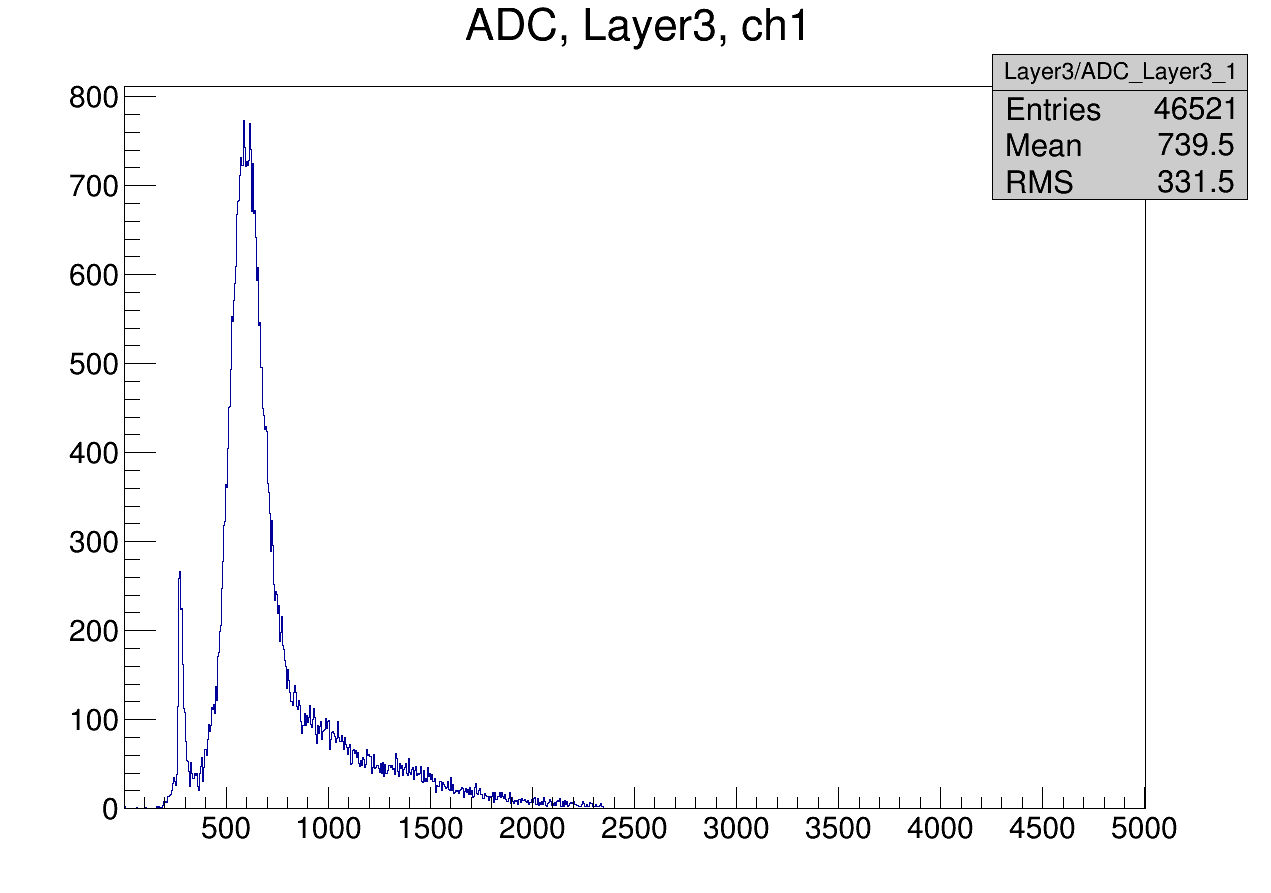
\includegraphics[width=0.95\textwidth]{../Pictures/ChannelModule-May2016.png} % Add an x-axis label to this too
	\caption{Histogram produced by \texttt{AHCALRawModuleChannel} showing an ADC spectrum of a single channel for one run. The pedestal can be seen at approximately 300 and the MIP peak at around 650.}
	\label{figure:aida/may2016/channelmodule}
\end{figure}

% We should use the ADC500 one here, because that makes sure that we remove the pedestal from the data and gives a better "signal" histogram
\begin{figure}[p]
	\centering
	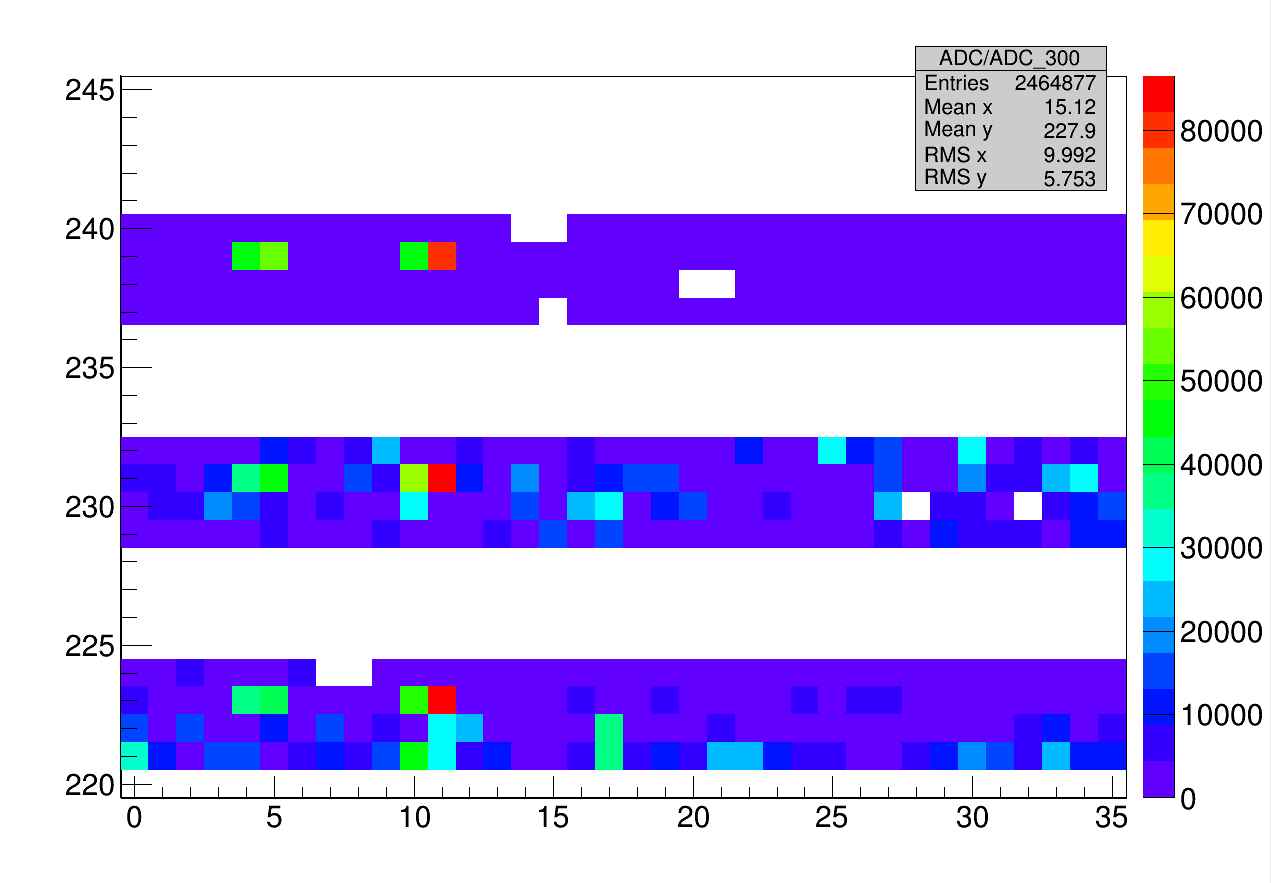
\includegraphics[width=0.85\textwidth]{../Pictures/GlobalModule-May2016.png} % Add axis labels: x is channel no., y is ChipID
	\caption{Histogram produced by \texttt{AHCALRawModuleGlobal} showing all ADCs exceeding 300 over a single run. Dead or nonresponsive channels are seen as white squares. The horizontal gaps are due to the fact that some ChipIDs were not present.}
	\label{figure:aida/may2016/globalmodule}
\end{figure}

The global module produced a 2D histogram containing cells for each channel, coloured for the \acrshort{ADC} in that channel. This didn't produce a hitmap as the geometry information was not available in this plot, but did allow easy identification of dead channels and channels that were in the beamspot. An example of this can be seen in Fig. \ref{figure:aida/may2016/globalmodule}.

Overall, once the monitoring had been set up and initial bugs and problems fixed, it became a routine tool of the testbeam. This was made easier by the usage of XML steering files for the monitoring interface canvases, allowing groups of plots and histograms to be automatically opened when the monitoring interface was started. This meant that with little effort, all information necessary for monitoring was easily available.

An example of the monitoring interface in use can be seen in Fig. \ref{figure:aida/may2016/overview}.

\begin{figure}[t]
	\centering
	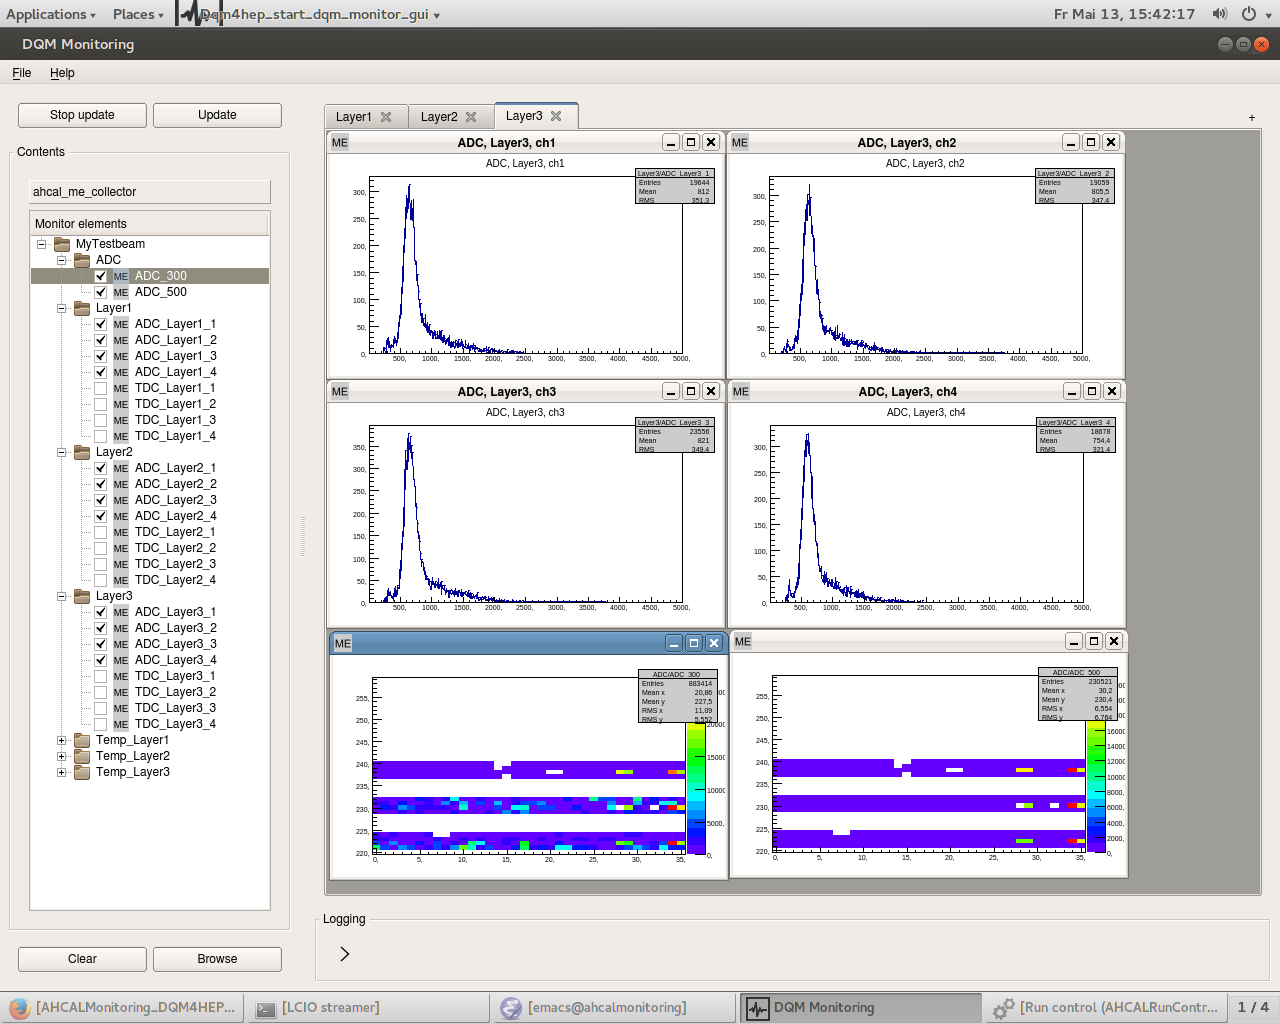
\includegraphics[width=0.95\textwidth]{../Pictures/PowerPulsingMipScans-May2016.png}
	\caption{A full screencapture from the May 2016 testbeam showing the monitoring interface in use during power pulsing tests, displaying a MIP scan.}
	\label{figure:aida/may2016/overview}
\end{figure}

\section{July 2016 DESY II}
The next usage of DQM4hep was a testbeam during July  2016, also at the DESY II facility. The testbeam was to be one week long, with a one-week preparation period. The primary goal for DQM4hep in this testbeam was to establish hitmaps of the calorimeter. This would give a visual representation of the layers, allowing identification of the beamspot, allowing dead or mis-calibrated channels to be identified visually.

Creating a hitmap for the AHCAL was nontrivial, as the information coming from the data acquisition device and stored in LCIO format did not encode location. Each channel was instead identified by its ``electronics number'' -- a combination of the ChipID of the board the channel was located on, and the number of the channel on that board.

Each layer was formed of four boards (each one with a ChipID), each of which contained sixteen layers. The orientation of the boards, which boards were in a layer, and the order of the layers in the stack were all changeable, so an additional requirement for the hitmap function was that it could take an external geometry file that could be changed or automatically generated. 

DQM4hep has internal functions for parsing XML data, so an XML file was chosen as the format to store the geometry data. By making this an XML file, it avoided hard-coding the geometry into the framework itself, allowing the geometry data to be changed at runtime. XML also has the benefit of being human-readable. The AHCAL team already used an internal format for the geometry file for offline processing after testbeams, which was constructed and converted into different fromats via a  shell script, so this could be replicated for the DQM4hep XML file.

For analysis modules needing geometry, the XML file was given as a required parameter for the steering file, which then built a C++ map of the correspondence between electronics number and $(i,j,k)$ co-ordinates of each channel in memory during initialisation. Then a function called \texttt{electronicsToIJK} was written that took the electronics number as the argument and returned the position of the channel in geometric co-ordinates. A further function was written, called \texttt{IJKToElectronics}, that performed the opposite operation, but this was not used. 

Using these new functions, another analysis module called \texttt{AHCALHitmap} was written that created a two dimensional histogram, with each bin representing a channel on the $x$ and $y$ axes for a single layer. This histogram was then filled with with the ADCs of that channel for the whole event, producing a hitmap.

The analysis modules for creating hitmaps were prepared ahead of the testbeam, and used extensively. They were used to identify channels that were dead or nonresponsive, as well as to confirm already-known nonresponsive channels.

\begin{figure}[p]
	\centering
	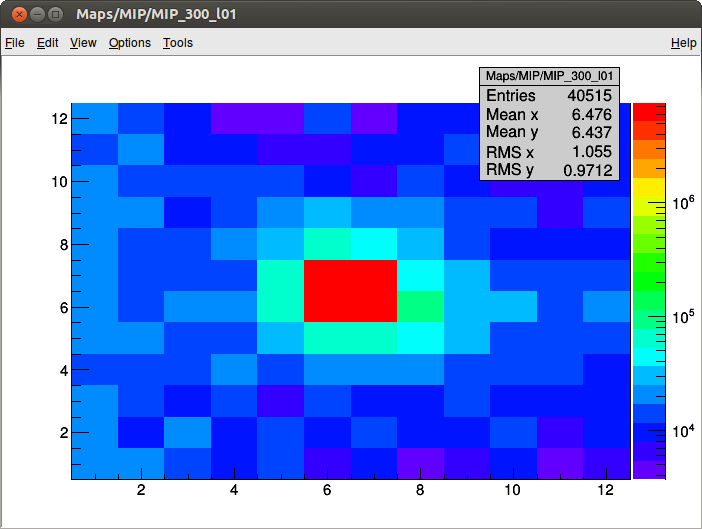
\includegraphics[width=0.95\textwidth]{../Pictures/AHCALHitmapSingle.png}
	\caption{A hitmap for a single layer during the July 2016 testbeam, showing all channels with ADCs higher than 300. The beamspot is clearly visible in the centre.}
	\label{figure:aida/july2016/single-hitmap}
\end{figure}

\begin{figure}[p]
	\centering
	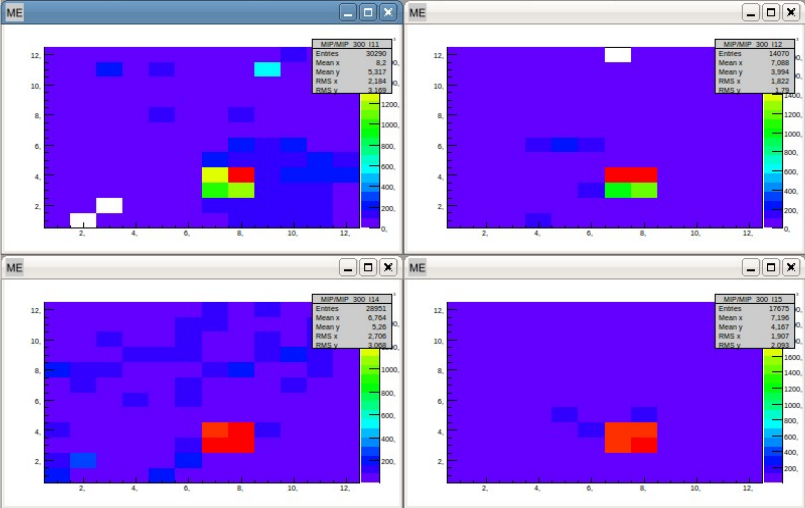
\includegraphics[width=0.95\textwidth]{../Pictures/AHCALHitmapFour.png}
	\caption{A collection of hitmaps for four layers in the stack during the July 2016 testbeam. The beamspot is visible, as are several dead or unresponsive channels in the top-left and top-right hitmaps.}
	\label{figure:aida/july2016/four-hitmap}
\end{figure}


\section{May 2017 at CERN SPS} % Wiki pages are here (http://flcwiki.desy.de/AHCALTestBeamCERN2017) but we ideally want an actual report for this.
During May 2017, testbeam time at CERN's Super Proton Synchrotron (SPS) facility was used for further tests for the AHCAL. One of the goals for this testbeam was to evaluate the performance of the power pulsing feature in magnetic fields up to 1.5T. The process of manufacturing the detector layers and boards was being automated, and a larger number of layers were available for this testbeam, so it also presented a way to test using a larger number of channels than before. 

Part of the programme for the testbeam was to use the electron and muon beams available at the SPS for calibrating the newly-produced layers, as well as doing an energy scan with a pion beam.

The monitoring with DQM4hep in this testbeam included analysis modules that monitored the individual channels of all 40 large layers, as well as producing hitmaps of several types, such as unweghted, ADC-weighted, and near-pedestal. Standalone modules monitoring the temperature of the detector hardware was also used. 

At this point in the testbeam process, the online monitoring system with DQM4hep had matured, partially due to the data format of the detector having been fixed for some time. Experience with running, using, and modifying the analysis modules had been disseminated throughout the team, and team members wrote their own analysis modules for producing plots.

Because of this, during the testbeam DQM4hep was used as intended -- as a tool for shifters to use to diagnose and troubleshoot problems with the beams or detectors. A specific expert on DQM4hep was not necessary, as enough people operating the testbeam understood DQM4hep to be able to modify analysis modules on the fly according to their needs.

% In previous testbeams, analysis modules that produced correlation plots were developed by other team members,

\begin{center}
	[Photographs from the installation and testbeam area go here]
\end{center}

\begin{center}
	[Plots from the testbeam]
\end{center}

%https://arxiv.org/pdf/1611.03627.pdf
%https://www.sciencedirect.com/science/article/pii/S0168900219304991
%https://www.sciencedirect.com/science/article/pii/S0168900217305703

\chapter{IDEA testbeams}
\label{chapter:ideatestbeam}

\epigraph{[new quote split \\ over two lines]}{[author]}

While \acrshort{DQM4hep} was intended from the beginning as a generic tool, it was developed largely within the AIDA-2020 collaboration, which also promoted a variety of standards and guidelines for data acquisition devices, data formats, etc. In addition to this, it was also only tested on calorimeter-type detectors within the \acrshort{CALICE} collaboration. To be sure that \acrshort{DQM4hep} was truly generic -- capable of adapting to \textit{any} detector -- it was necessary to test it on a wider variety of detectors outside of the AIDA-2020 and \acrshort{CALICE} collaborations.

An ideal opportunity arose for this in the form of the \acrshort{IDEA} testbeam. This testbeam was run by a collaboration of Italian and American universities working on four different particle physics detectors of different types, intending to run a single combined testbeam of all four instruments at the \acrshort{CERN} \acrshort{SPS} in September 2018. \acrshort{DQM4hep} was offered as a possible unified monitoring solution that could integrate information from all four detectors into the same tool. This provided convenience for the teams operating the testbeam and detectors, and an extremely valuable opportunity to test \acrshort{DQM4hep} out of its established operating range.

\section{Introduction}
The combined testbeam took place between in September 2018 at the \acrshort{CERN} \acrshort{SPS} beamline facility. The testbeam itself lasted a week, from the 5th-12th September, with a preparation period of one week before this for installation, calibration, etc. [...]

\subsection*{Detectors at the combined testbeam}
The combined testbeam comprised four separate dectors: a calorimeter, a muon detector and preshower, a drift chamber, and a silicon photomultiplier. One of the biggest challenges involved in the testbeam was operating these four different detectors [...]

\subsubsection{RD52 calorimeter} % Another reference: https://arxiv.org/pdf/1703.09120.pdf
The \acrfull{DREAM} calorimeter, also called the RD52 calorimeter, is a dual-readout calorimeter built, developed and tested by the RD52 collaboration by researchers based in universities at Gagliari, Cosenza, Pavia, Pisa, Rome, Iowa State and Texas Tech. 

The aim of the calorimeter is to use both the \v{C}erenkov and scintillator techniques simultaneously (hence ``dual-readout'') to improve calorimetry, especially using calorimeters to measure four-vectors of jets and single hadrons, which suffer a reduced precision compared to electrons and photons. By comparing signals from \v{C}erenkov light and scintillator light, the electromagnetic shower fraction can be measured on an event-by-event basis, eliminating the effects of fluctuations. %Reference here: https://iopscience.iop.org/article/10.1088/1742-6596/404/1/012068/pdf

%-Nine lead modules (9.3x9.3x150cm^3)
%-Sampling fraction 5%, PMT readout
%-Hadronic energy resolution in 4pi geometry should be 30%/sqrt(E)

\subsubsection{Muon chamber and preshower}
[...]

%Muon chamber
%-One triple-GEM, same as preshower
%-Two micro-RWELL 10x10cm^2 (40 micron spatial resolution, rates up to 10MHz/cmm^2)

%Preshower
%-Lead absorber with fixed 5mm layer, but can vary from 1 to 2.5 X_0
%-Two triple-GEM detectors
%-10x10cm^2 surface area, strip readout, 650 micron pitch
%-Ar/CO2/CF4 gas used for testbeam
%-Efficiency 97% based on previous testbeams
%-Spatial resolution 100 microns

\subsubsection{Silicon photomultiplier GEM}
[...]

\subsubsection{Drift chamber}
[...]

%-12 layers, with 12 1x1cm^2 drift cells per layer
%-144 channels total
%-resolution is 100 micron in x-y, 1mm in z

\subsubsection{Ancillary detectors}

%-Two DWCs before and after drift chamber, for beam particle position, leakage, for particle ID

\section{Monitoring}
[...]

Existing monitoring within the \acrshort{DREAM} collaboration could produce accurate histograms from raw data using ROOT, creating plots of the energy spectra of each detector channel per event, along with [...]. This facility was reproduced in \acrshort{DQM4hep} quickly using for-loops in both the C++ code and \acrshort{XML} steering files, allowing this to be done with comparatively little code.

\subsection{File readers}
Writing file readers for the different detectors meant first understanding the structure of their data and file types. Once data has arrived from the data acquisition device, each of the detectors wrote to a different `raw' format. However, the RD52 calorimeter, drift chamber, and muon and preshower all produced ROOT ntuple files as part of their data acquisition process, in addition to different file formats. It was decided to use these ROOT ntuples as the file format to read into \acrshort{DQM4hep}, as due to support for ROOT within the framework, reading data from ROOT ntuples is simpler.

For each of these three instruments a file reader was developed that walked through the ROOT trees, extracting data from the leaves event-by-event, then converted it to \acrshort{DQM4hep}'s inbuilt \texttt{GenericEvent} format. Choosing to make them into GenericEvents meant that there was no need to implement an additional event type, simplifying the connection between the file readers and analysis modules. The GenericEvent type was also easily suited to the type of data, as the majority of the data were series of numbers, which were easily converted into C++ vectors to store in the GenericEvent.

An additional motivation for using the ROOT ntuple as the data source was that some of the file type, notably the drift chamber, had not finalised their data structure at the beginning of the testbeam. Using the higher-level structure provided by a ROOT file would be easier to change in the future than reading in data in a binary, hex, text or \acrshort{CSV} format.

For the silicon photomultiplier \acrshort{GEM} data, the ``raw'' data format was a text file, containing an \acrshort{XML} header followed by a large amount of data in \acrfull{CSV}. This file could be loaded directly into \acrshort{DQM4hep}, the \acrshort{XML} header separated and parsed with \acrshort{DQM4hep}'s internal \acrshort{XML} parsing libraries, and the remaining data parsed. The comma-separated values could be easily parsed using the \texttt{dqm4hep::core::tokenize} function, which takes a string, a delimiter, and a vector, and parses the string into values separated by the delimiter, loading them into the vector. This made extracting the \acrshort{GEM} data extremely simple, even in this format. It also allowed the parameters in the \acrshort{XML} header, which included run numbers and physical information of the detector, to be passed into DQM4hep and the analysis module, using the \texttt{core::Run} object type.

\subsection{Analysis modules}
During the course of the testbeam, four analysis modules were developed, one for each detector. To begin with, these were `dummy' modules -- analysis modules that receive events then do nothing. Dummy modules like this are required to run file readers offline, but are simple to create as they can be produced from a template with minimal changes.

Once the file reader for the RD52 calorimeter was complete, the dummy analysis module for this detector was then changed into a functional module, \texttt{RD52MainModule}, to produce plots from the data. The RD52 was chosen as it was the most data-rich of the detectors in the testbeam, and also contained the ancillary detectors, which allow particle selection efficiencies to be studied.

During the course of the testbeam, the \texttt{RD52MainModule} was developed to read in and arrange data from the ROOT ntuples and arrange them into distinct vectors for the \acrshort{ADC}s, \acrshort{TDC}s, pedestals, and ancillaries. Following this, pedestal subtraction of all \acrshort{ADC} and \acrshort{TDC} channels was completed. Then the malfunctioning tiles and electronics that meant data had to be re-routed through other available channels was integrated so that the \acrshort{ADC} information in the analysis module represented the full state of the detector was completed. 

There was insufficient time at the testbeam to develop the monitoring more complex than this, but further development continued offline with saved data from the testbeam to continue the proof-of-concept. This will be discussed in more detail in the following section.

\section{Results}
Monitoring within \acrshort{DQM4hep} was able to replicate all the existing monitoring solutions, combining the monitoring tools for all four detector systems into one framework. [...] However due to time constraints, more complex monitoring such as online processing was not implemented during the testbeam. [...] 

Following the testbeam, it was decided that \acrshort{DQM4hep} could be used to perform some offline analysis functions in addition to the work at the testbeam, as a further proof of its ability to do this at testbeams. [...]

Several analysis goals were outlined to attempt to implement in \acrshort{DQM4hep}. These were performing the tower \acrshort{ADC} calibration, the \acrshort{ADC} to energy calibration, and particle selection efficiencies. 

\subsection{Tower ADC calibration}
[...]

Due to a large number of tasks for setting up the testbeam, performing a calibration of the individual towers' high voltages was not possible, so the calorimeter \acrshort{ADC}s were not calibrated to each other [?]. In order to fix this, [...]

Two sets of calibration runs were performed. The first set covered Towers 1-29 using an 80 GeV secondary beam ($\pi$ and $e^{-}$), with the beam pointed at each tower in sequence for 29 runs. The second set used a 20 GeV electon beam, covering Towers 30-36 plus Tower 15. Tower 15 recieved runs in both sets in order to calibrate the two sets to each other. 

[...] The run numbers corresponding to each tower is given in Table \ref{table:idea/calibrationruns}.

\begin{table}[h]
\centering
	\begin{tabular}{ c c | c c }
	\hline \hline
	\textbf{Tower} & \textbf{Run No.} & \textbf{Tower} & \textbf{Run No.} \\ \hline \hline
	 1 & 12545 & 16 & 12526 \\
	 2 & 12556 & 17 & 12567 \\
	 3 & 12558 & 18 & 12633 \\
	 4 & 12560 & 19 & 12591 \\
	 5 & 12601 & 20 & 12612 \\
	 6 & 12638 & 21 & 12530 \\
	 7 & 12598 & 22 & 12528 \\
	 8 & 12514 & 23 & 12569 \\
	 9 & 12518 & 24 & 12639 \\
	10 & 12521 & 25 & 12610 \\
	11 & 12600 & 26 & 12609 \\
	12 & 12636 & 27 & 12607 \\
	13 & 12539 & 28 & 12604 \\
	14 & 12628 & 29 & 12602 \\
	15 & 12512 &    &    \\ \hline
	\end{tabular}
	\caption{Table of the run numbers and corresponding tower numbers for the calibration runs.}
	\label{table:idea/calibrationruns}
\end{table}

%
%\begin{table}[h]
%\centering
%	\begin{tabular}{ c c c c }
%	\hline \hline
%	\textbf{Tower} & \textbf{Run No.} & \textbf{Beam energy} & \textbf{Beam type} \\ \hline \hline
%	 1 & 12545 & 80 GeV & secondary \\
%	 2 & 12556 & 80 GeV & secondary \\
%	 3 & 12558 & 80 GeV & secondary \\
%	 4 & 12560 & 80 GeV & secondary \\
%	 5 & 12601 & 80 GeV & secondary \\
%	 6 & 12638 & 80 GeV & secondary \\
%	 7 & 12598 & 80 GeV & secondary \\
%	 8 & 12514 & 80 GeV & secondary \\
%	 9 & 12518 & 80 GeV & secondary \\
%	10 & 12521 & 80 GeV & secondary \\
%	11 & 12600 & 80 GeV & secondary \\
%	12 & 12636 & 80 GeV & secondary \\
%	13 & 12539 & 80 GeV & secondary \\
%	14 & 12628 & 80 GeV & secondary \\
%	15 & 12512 & 80 GeV & secondary \\
%	15 & 12659 & 20 GeV & electrons \\
%	16 & 12526 & 80 GeV & secondary \\
%	17 & 12567 & 80 GeV & secondary \\
%	18 & 12633 & 80 GeV & secondary \\
%	19 & 12591 & 80 GeV & secondary \\
%	20 & 12612 & 80 GeV & secondary \\
%	21 & 12530 & 80 GeV & secondary \\
%	22 & 12528 & 80 GeV & secondary \\
%	23 & 12569 & 80 GeV & secondary \\
%	24 & 12639 & 80 GeV & secondary \\
%	25 & 12610 & 80 GeV & secondary \\
%	26 & 12609 & 80 GeV & secondary \\
%	27 & 12607 & 80 GeV & secondary \\
%	28 & 12604 & 80 GeV & secondary \\
%	29 & 12602 & 80 GeV & secondary \\
%	30 & 12664 & 20 GeV & electrons \\
%	31 & 12677 & 20 GeV & electrons \\
%	32 & 12672 & 20 GeV & electrons \\
%	33 & 12671 & 20 GeV & electrons \\
%	34 & 12670 & 20 GeV & electrons \\
%	35 & 12669 & 20 GeV & electrons \\
%	36 & 12667 & 20 GeV & electrons \\ \hline
%	\end{tabular}
%	\caption{Table of the run numbers and corresponding tower numbers for the calibration runs.}
%	\label{table:idea/calibrationruns}
%\end{table}

The process for calibrating the towers was to make a histogram of the \acrshort{ADC}s registered in a tower, only in the run where the beam was centered on them, in order to find the mean and standard deviation. These histograms were then combined to show the overall responses of the entire set of calibration runs, which visualises the differences between the Towers. These can be seen in Fig. \ref{figure:testbeam/results/calibrationbefore}. 

Since Tower 15 was present in both runs, this was chosen as the reference, and all the other towers were given a coefficient that leveled their mean \acrshort{ADC} to the same value as Tower 15, in both sets of calibration runs. The \acrshort{ADC} values for each tower are then multiplied by their calibration coefficient. [...] [Difference between scintillator and Cherenkov] [...] The calibration coefficients are shown on Table \ref{table:idea/calibrationcoeffs}.

\begin{table}[h]
\centering
	\begin{tabular}{ c c | c c }
	\hline \hline
	\textbf{Tower} & \textbf{Coefficient} & \textbf{Tower} & \textbf{Coefficient} \\ \hline \hline
	 1 & x & 16 & x \\
	 2 & x & 17 & x \\
	 3 & x & 18 & x \\
	 4 & x & 19 & x \\
	 5 & x & 20 & x \\
	 6 & x & 21 & x \\
	 7 & x & 22 & x \\
	 8 & x & 23 & x \\
	 9 & x & 24 & x \\
	10 & x & 25 & x \\
	11 & x & 26 & x \\
	12 & x & 27 & x \\
	13 & x & 28 & x \\
	14 & x & 29 & x \\
	15 & x &    &    \\ \hline
	\end{tabular}
	\caption{Table of tower numbers and their calibration coefficients.}
	\label{table:idea/calibrationcoeffs}
\end{table}

\begin{figure}[h]
	\centering
	
\includegraphics[width=0.65\textwidth]{../Pictures/Placeholder.png}
	\caption{The plot of \acrshort{ADC}s for each tower before calibration.}
	\label{figure:testbeam/results/calibrationbefore}
\end{figure}

\begin{figure}[h]
	\centering
	
\includegraphics[width=0.65\textwidth]{../Pictures/Placeholder.png}
	\caption{Comparison of the calibration plots for the \acrshort{ADC}s before and after calibration.}
	\label{figure:testbeam/results/calibrationafter}
\end{figure}

\subsection{ADC to energy calibration}
[...] It was known from prior testbeams that the response of the calorimeter was linear with ADC, therefore the energy calibration could be extrapolated from a single datapoint. [...]

\subsection{Particle selection efficiencies}
An important result for the calorimeter was determining the efficiency with which it could determine the beam composition and select for certain types of particles based on kinematic properties. The calorimeter was designed with a set of ancillary detectors to help discriminate between particle of different types. These provide a first selection of different particles, allowing us to use kinematic properties from the calorimeter itself to perform a second particle selection, and then compare the two.

The two ancillary detectors used for particle selection are the muon trigger and ...]

[...]

\subsubsection{Using the calorimeter}
[...]

One of the first steps is using the RD52 calorimeter data to find the energy ratio $R$ for each event:

\begin{displaymath}
	R = \frac{E_1}{\sum_{i=1}^{n} E_i}
\end{displaymath}

where $E_i$ is the energy of the $i^{th}$ most energetic channel in the event and $n$ is a nonzero integer. The choice of $n$ [...]. Once the ratio $R$ is calculated, a plot can be made of $E_{total}$ vs. $R$ for an entire run that shows separation of electrons from muons and pions -- see Fig. \ref{figure:testbeam/results/EvR}.

% Replace this diagram with the updated one (though probably *after* we've normalised for beam energy).
% Also, Run 12709 is an electron run, not a hadron run!

\begin{figure}[h]
	\centering
	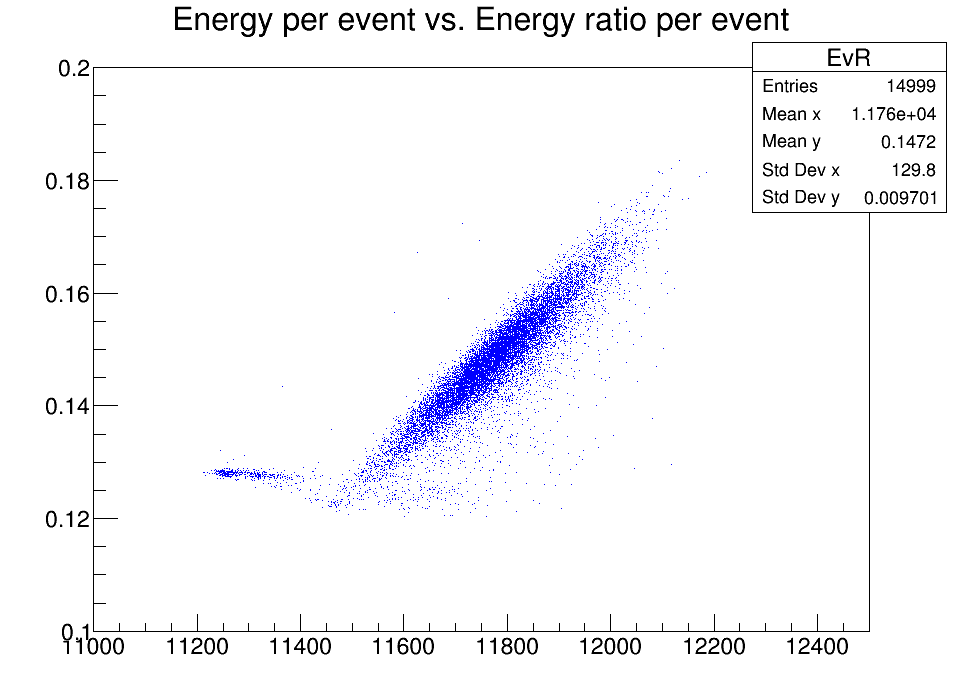
\includegraphics[width=0.65\textwidth]{../Pictures/12709-EvR.png}
	\caption{Plot of $E$ against $R$ for the secondary hadron beam with $n = 10$ (Run 12709).}
	\label{figure:testbeam/results/EvR}
\end{figure}

An appropriate cut can be used to select electron events. [Information about the cut]. Adding in the information from the RD52's muon trigger, muons and pions can then also be separated. Using both the cut and the muon trigger, we can thus produce spectra for each individual type of particle in the run.

[...]

The main goal of the data analysis is to characterise the response of the detector, and to measure the selection efficiencies of the detectors to various particle types. Once this is done, this will also give us a detailed account of the beam composition during each of the runs, which can be used for further work.

In order to do this, several ways to select for different particle types are necessary. The first way was using the preshower detector and muon trigger, which are both designed to discriminate between electrons and muons (respectively), with a high selection efficiency. These are used to create ``reference'' samples, [...]

The second way is to perform a kinematic selection using variables from the calorimeter. This is done using the E vs. R plot (normalised for beam energy) to select a region corresponding to a certain particle type. For example, the plot below shows this plot for Run [xxx] (X GeV hadrons) with the regions corresponding to hadrons and electrons highlighted. These regions overlap, meaning that attempting to select for hadrons using an ellipse around that region will also result in a non-insignificant number of electrons also being selected.

In order to perform a pure selection using the calorimeter, an extremely tight cut was used, focusing on the red spot at the centre of the hadron region. This ensures that the majority of events that pass the cut are hadrons, giving a high-purity selection. The purity of this selection can be assessed by using the appropriate preshower or muon trigger, excluding all non-hadron particles, and comparing the two numbers. If $N_{K}$ is the number of particles passing the selection with only the kinematic cut, and $N_{K+T}$ is the number of particles passing \emph{both} the kinematic cut and the triggers, then the selection efficiency for hadrons $\epsilon_{hadron}$ is given by:

\begin{displaymath}
	\epsilon_{hadron} = \frac{N_{K+T}}{N_{K}}
\end{displaymath}

This was then done with the same process for electrons and muons, to obtain the individual selection efficiencies. % Should probably go through the process with the actual cut values itself.

% Results of this selection, and the matrix?

\chapter{Physics studies for the Compact Linear Collider}
\label{chapter:analysis}

\epigraph{Somewhere, something incredible is waiting to be known.}{Carl Sagan}

One of the primary goals of future lepton colliders is to become ``Higgs factories'' -- machines that can produce large numbers of Higgs bosons in a variety of final states, allowing the Higgs sector of the \acrlong{SM} to be probed with unprecedented accuracy and coverage.

One of the best way to examine the Higgs sector is via the production of Higgs bosons in association with top quarks. The coupling between these two particles -- the top-Higgs Yukawa coupling -- is the strongest Higgs coupling of all, making it one of the easiest ways to examine the properties of the Higgs and its couplings. 

An important process used to study the coupling between the Higgs and the top is the so-called $tth$ process:
$$
e^+ e^- \rightarrow t\overline{t}h
$$

The production of two top quarks in association with a Higgs makes this an ideal probe for this coupling. However, the decay channels of this process vary -- each top quark can decay in one of two ways. It can decay \textit{hadronically} into a quark-antiquark pair, where one quark is up-type and the other is down-type; or it can decay \textit{leptonically} into a lepton of the same charge as the W and a neutrino of the same flavour, with one being an antiparticle (e.g. $e^- \overline{\nu}_e$ or $\mu^+ \nu_\mu$). The total branching ratio of hadronic decays is 68\%, and the total branching ratio of the leptonic decays is 32\%. The decay processes of the W are: % Ref for old BRs: http://pdg.lbl.gov/2013/listings/rpp2013-list-w-boson.pdf

$$
W^+ \rightarrow q\overline{q}
$$
$$
W^+ \rightarrow \ell^+ \nu
$$
$$
W^- \rightarrow q\overline{q}
$$
$$
W^- \rightarrow  \ell^- \nu
$$

where $q\overline{q}$ denotes the quark-antiquark pair and $\ell \nu$ denotes the lepton-neutrino pair. Thus there are three possible final states:
$$
e^+ e^- \rightarrow t\overline{t}h \rightarrow q\overline{q}q\overline{q}b\overline{b}
$$
$$
e^+ e^- \rightarrow t\overline{t}h \rightarrow \ell \nu \ell \nu b \overline{b}
$$
$$
e^+ e^- \rightarrow t\overline{t}h \rightarrow \ell \nu q \overline{q} b \overline{b}
$$

The upshot of this is that in order to perform accurate analysis of this process, jet energy resolution and jet reconstruction is of primary importance, as the majority of the decays will be via the hadronic channel. As discussed in Chapter \ref{chapter:colliders}, the detector concepts for future lepton colliders are designed to focus on jet energy resolution and jet reconstruction, and utilise particle flow to augment this.

This chapter describes an analysis performed to attain a precision on the measurement of the top-Higgs Yukawa coupling at the \acrfull{CLIC} experiment at a centre-of-mass energy of $\sqrt{s} = 1.4TeV$, using the CLIC\textunderscore SiD detector concept. This analysis focuses specifically on the hadronic channel, and when taken in combination with a similar analysis of the semi-leptonic channel performed by Yixuan Zhang\refthis allows calculation of the precision on the top-Higgs Yukawa coupling.

\begin{figure}[h]
	\centering
	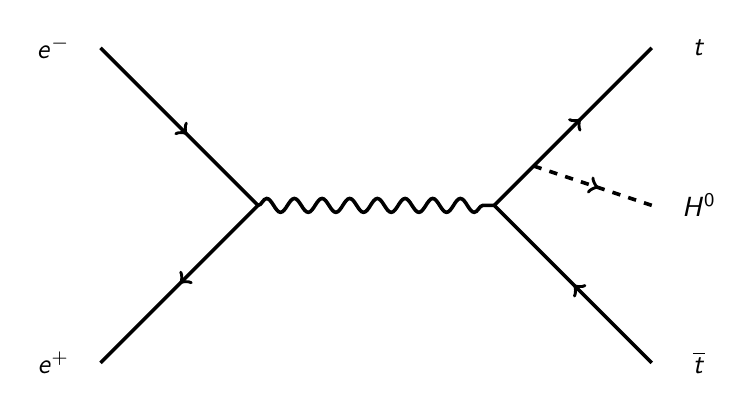
\begin{tikzpicture}[line width=1.3 pt,scale=2]
		\draw[fermion]  (0,1) -- (1,0) ;
		\draw[fermionbar]  (0,-1) -- (1,0) ;
		\draw[vector]  (1,0) -- (2.5,0) ;
		\draw[fermion]  (2.5,0) -- (3.5,1) ;
		\draw[fermionbar]  (2.5,0) -- (3.5,-1) ;
		\draw[scalar]  (2.75,0.25) -- (3.5,0.) ;
		\node at (-0.3, 1) {$e^-$};
		\node at (-0.3, -1) {$e^+$};
		\node at (3.8, 1) {$t$};
		\node at (3.8, -1) {$\overline{t}$};
		\node at (3.8, 0) {$H^0$};
	\end{tikzpicture} 
	\caption{A Feynman diagram of the $tth$ event.}
	\label{figure:physics/SM/feynman-tth}
\end{figure}

\section{Anatomy of the $tth$ event}
%Papers for top-Higgs Yukawa coupling, tth, and the analysis process: 
%https://arxiv.org/pdf/1807.02441.pdf
%http://cds.cern.ch/record/1690648/files/LCD_tth_note.pdf?version=1
%http://cds.cern.ch/record/1982243/files/CLICdp-Note-2015-001.pdf?version=1
%https://arxiv.org/pdf/1608.07538.pdf

The $tth$ event has three possible final states, defined by the decay channel of the W bosons produced by the top quarks. The decay of a top quark will always produce a W boson and a bottom quark, while the W boson can decay one of two ways. Since \textit{which} W produces certain decay products does not matter, there are three possible combinations that can be seen in Table \ref{table:physics/final-states}.

\begin{table}[h]
\centering
	\begin{tabular}{ c c c }
	\hline \hline
	Decay Channel & Final State & Branching Ratio \\ \hline \hline
	Fully hadronic & $q\overline{q}q\overline{q}b\overline{b}$ & 46\% \\ \hline
	Semi-hadronic &  $\ell \nu q\overline{q}b\overline{b}$ & 45\% \\ \hline
	Fully leptonic & $\ell \nu \ell \nu b\overline{b}$ & 9\% \\ \hline 
	\end{tabular}
	\caption{Blah blah}
	\label{table:physics/final-states}
\end{table}

Given it's extremely low branching ratio relative to the other channels, the fully leptonic state is not considered in this analysis. Extended Feynman diagrams of the fully hadronic and semi-leptonic final states are shown in Figs. \ref{figure:physics/SM/feynman-tth-hadronic} and \ref{figure:physics/SM/feynman-tth-semileptonic}

[...]

There is another contribution to the tth final state in the higgstrahlung process. In this case, the electron and positron form a Z or $\gamma *$ as an intermediate before producing a $t \overline{t}$ pair. A Higgs boson is radiated off the $Z/\gamma *$, resulting in the same final tth state but without a direct interaction between the Higgs and top quark (see Fig. \ref{figure:physics/SM/higgstrahlung}). This means that the higgstrahlung process is not sensitive to the top-Higgs Yukawa coupling, and this must be taken into account when calculating the total cross-section of the tth process.

In order to correct for this, [...]
	
\begin{figure}[h]
	\centering
	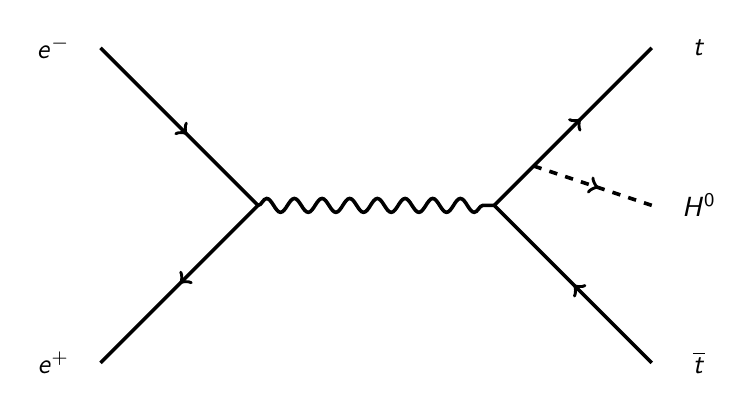
\begin{tikzpicture}[line width=1.3 pt,scale=2]
		\draw[fermion]  (0,1) -- (1,0) ;
		\draw[fermionbar]  (0,-1) -- (1,0) ;
		\draw[vector]  (1,0) -- (2.5,0) ;
		\draw[fermion]  (2.5,0) -- (3.5,1) ;
		\draw[fermionbar]  (2.5,0) -- (3.5,-1) ;
		\draw[scalar]  (2.75,0.25) -- (3.5,0.) ;
		\node at (-0.3, 1) {$e^-$};
		\node at (-0.3, -1) {$e^+$};
		\node at (3.8, 1) {$t$};
		\node at (3.8, -1) {$\overline{t}$};
		\node at (3.8, 0) {$H^0$};
	\end{tikzpicture} 
	\caption{A Feynman diagram of the higgstrahlung process.}
	\label{figure:physics/SM/higgstrahlung}
\end{figure}

\begin{figure}
	\centering
	\begin{tikzpicture}[line width=1.3 pt,scale=2.25]
		% Initial electrons	
		\draw[fermion]  (0,1) -- (1,0) ;
		\draw[fermionbar]  (0,-1) -- (1,0) ;
		% The central bar
		\draw[vector]  (1,0) -- (2.5,0) ;
		% The final top quarks
		\draw[fermion]  (2.5,0) -- (3.5,1) ;
		\draw[fermionbar]  (2.5,0) -- (3.5,-1) ;
		% The Higgs boson radiating off
		\draw[scalar]  (2.75,0.25) -- (3.5,0.) ;
		% The W+ and bottom quark coming off the top quark
		\draw[vector]  (3.5,1) -- (4.5,1.5) ;
		\draw[fermion]  (3.5,1) -- (4.5,0.5) ;
		% The W- and anti-bottom quark coming off the anti-top quark
		\draw[fermionbar]  (3.5,-1) -- (4.5,-0.5) ;
		\draw[vector]  (3.5,-1) -- (4.5,-1.5) ;
		% The quark-antiquark pair coming off the W+
		\draw[fermion]  (4.5, 1.5) -- (5.5,2) ;
		\draw[fermion]  (4.5, 1.5) -- (5.5,1) ;
		% The quark-antiquark pair coming off the W-
		\draw[fermionbar]  (4.5, -1.5) -- (5.5,-1) ;
		\draw[fermionbar]  (4.5, -1.5) -- (5.5,-2) ;
		% Labels
		\node at (-0.3, 1) {$e^-$};
		\node at (-0.3, -1) {$e^+$};
		\node at (3.8, 1) {$t$};
		\node at (3.8, -1) {$\overline{t}$};
		\node at (3.8, 0) {$H^0$};
		\node at (5.0, 1.5) {$W^+$};
		\node at (4.8, 0.5) {$b$};
		\node at (4.8, -0.5) {$\overline{b}$};
		\node at (5.0, -1.5) {$W^-$};
		\node at (5.8,2) {$q$};
		\node at (5.8,1) {$\overline{q}$};
		\node at (5.8,-1) {$q$};
		\node at (5.8,-2) {$\overline{q}$};
	\end{tikzpicture} 
	\caption{An extended Feynman diagram of the tth event, showing the fully-hadronic decay channel with the final state $q\overline{q}q\overline{q}b\overline{b}$, where $q$ and $\overline{q}$ indicate a quark-antiquark pair. \newline}
	\label{figure:physics/SM/feynman-tth-hadronic}
	\begin{tikzpicture}[line width=1.3 pt,scale=2.25]
		% Initial electrons
		\draw[fermion]  (0,1) -- (1,0) ;
		\draw[fermionbar]  (0,-1) -- (1,0) ;
		% The central bar
		\draw[vector]  (1,0) -- (2.5,0) ;
		% The final top quarks
		\draw[fermion]  (2.5,0) -- (3.5,1) ;
		\draw[fermionbar]  (2.5,0) -- (3.5,-1) ;
		% The Higgs boson radiating off
		\draw[scalar]  (2.75,0.25) -- (3.5,0.) ;
		% The W+ and bottom quark coming off the top quark
		\draw[vector]  (3.5,1) -- (4.5,1.5) ;
		\draw[fermion]  (3.5,1) -- (4.5,0.5) ;
		% The W- and anti-bottom quark coming off the anti-top quark
		\draw[fermionbar]  (3.5,-1) -- (4.5,-0.5) ;
		\draw[vector]  (3.5,-1) -- (4.5,-1.5) ;
		% The lepton-neutrino pair coming off the W+
		\draw[fermion]  (4.5, 1.5) -- (5.5,2) ;
		\draw[fermion]  (4.5, 1.5) -- (5.5,1) ;
		% The quark-antiquark pair coming off the W-
		\draw[fermionbar]  (4.5, -1.5) -- (5.5,-1) ;
		\draw[fermionbar]  (4.5, -1.5) -- (5.5,-2) ;
		% Labels
		\node at (-0.3, 1) {$e^-$};
		\node at (-0.3, -1) {$e^+$};
		\node at (3.8, 1) {$t$};
		\node at (3.8, -1) {$\overline{t}$};
		\node at (3.8, 0) {$H^0$};
		\node at (5.0, 1.5) {$W^+$};
		\node at (4.8, 0.5) {$b$};
		\node at (4.8, -0.5) {$\overline{b}$};
		\node at (5.0, -1.5) {$W^-$};
		\node at (5.8,2) {$\ell$};
		\node at (5.8,1) {$\nu$};
		\node at (5.8,-1) {$q$};
		\node at (5.8,-2) {$\overline{q}$};
	\end{tikzpicture} 
	\caption{An extended Feynman diagram of the tth event, showing the semi-hadronic decay channel  with the final state $\ell\nu q\overline{q}b\overline{b}$, where $\ell$ and $\nu$ indicate a lepton-neutrino pair.}
	\label{figure:physics/SM/feynman-tth-semileptonic}
\end{figure}

\section{Physics generation and samples}
The Monte Carlo samples were generated predominantly using Whizard 1.95, though for the Higgs events, Physsim was used due to technical constraints of Whizard [ref?]. All samples were simulated at $\sqrt{s} = 1.4TeV$ using unpolarised beams, assuming an integrated luminosity of 1.5 ab\textsuperscript{-1} and a light \acrlong{SM} Higgs boson with mass of 125 GeV. See Table \ref{table:physics/SM/generatedsamples} for a summary of all of the used samples. The first two rows are the tth signal channels, all other rows are backgrounds. The number of jets refers to the number of jets in the final state that have come from the decay of the top quark pair. The number of events in 1.5 ab\textsuperscript{-1} has been calculated from the integrated luminosity and sample weight.

\begin{table}[htp]
\centering
	\begin{tabular}{ c l c r r }
	\hline \hline
	ProdID & Process & Cross-section (fb) & Sample weight & Events in 1.5 ab\textsuperscript{-1} \\ \hline \hline
	2435 & $t\overline{t}h$, 6 jets, $h \rightarrow b\overline{b}$ & 0.431 & 0.03 & 647 \\
	2441 & $t\overline{t}h$, 4 jets, $h \rightarrow b\overline{b}$ & 0.415 & 0.03 & 623 \\ \hline
	2429 & $t\overline{t}h$, 2 jets, $h \rightarrow b\overline{b}$ & 0.100 & 0.006 & 150 \\

	2438 & $t\overline{t}h$, 6 jets, $h \not\rightarrow b\overline{b}$ & 0.315 & 0.02 & 473	 \\
	2444 & $t\overline{t}h$, 4 jets, $h \not\rightarrow b\overline{b}$ & 0.303 & 0.02 & 455 \\
	2432 & $t\overline{t}h$, 2 jets, $h \not\rightarrow b\overline{b}$ & 0.073 & 0.004 & 110 \\

	2450 & $t\overline{t}Z$, 6 jets & 1.895 & 0.1 & 2843 \\
	2453 & $t\overline{t}Z$, 4 jets & 1.825 & 0.1 & 2738 \\
	2447 & $t\overline{t}Z$, 2 jets & 0.439 & 0.03 & 659 \\
	
	2423 & $t\overline{t}b\overline{b}$, 6 jets & 0.549 & 0.03 & 824 \\
	2426 & $t\overline{t}b\overline{b}$, 4 jets & 0.529 & 0.03 & 794 \\
	2420 & $t\overline{t}b\overline{b}$, 2 jets & 0.127 & 0.008 & 191 \\

	2417 & $t\overline{t}$ & 125.8 & 1.5 & 203700 \\ \hline

	\end{tabular}
	\caption{Table of all signal and background samples used for this analysis.}
	\label{table:physics/SM/generatedsamples}
\end{table}

\section{Detector models}
[...]

[...] henceforth referred to as CLIC\textunderscore SiD.

\section{Analysis method}
The first and most important step off the analysis is to determine which jets originate from the Higgs boson, [...] The invariant mass of the Higgs boson can be determined by summing the invariant masses of pairs of bottom quarks and computing the $\chi^2$ for each possible combination; the combination with the lowest $\chi^2$ shows the pair that has decayed from the Higgs boson. [...]

\begin{equation}
  \centering
	\chi^2 = \frac{(m_{ij} - m_W)^2}{\sigma^2_W} + \frac{(m_{ijk} - m_t)^2}{\sigma^2_{t_1}} + \frac{(m_{ijk} - m_t)^2}{\sigma^2_{t_2}} + \frac{(m_{lm} - m_H)^2}{\sigma^2_H}
\label{eq:chi-square}
\end{equation}

A similar equation is used for the semi-leptonic channel, removing one of the terms for the top quark mass.

\subsection{Sample processing}
The first step of processing the samples is the initial jet clustering. This is done using the $k_t$ algorithm with parameters [?], using an exclusive clustering mode to form 8 jets -- 6 jets from the produced quarks and 2 beam jets. The $k_t$ algorithm is used over choices like anti-$k_t$ and Valencia, because the important features are the \emph{relative} shapes of the jets, rather than absolute properties, so there is no need to use more computationally-intensive [is this true?] algorithms.

Once initial jet clustering is finished, a Marlin processor that finds isolated leptons is used. It searches for either 0, 1, or 2 isolated leptons, and this information can be used to make decisions about whether to process the event already:

\begin{table}[htp]
\centering
	\begin{tabular}{ | c | l | l | }
	\hline
	Leptons & Channel & Action \\ \hline
	0 & Fully hadronic & Use for fully hadronic analysis \\ \hline
	1 & Semi-leptonic & Use for semi-leptonic analysis \\ \hline
	2 & Fully leptonic & Discard \\ \hline
	\end{tabular}
\end{table}

Following this, the two beam jets are removed from the processing, and a further step of jet re-clustering is performed, using the Durham algorithm, to [...] [Why is this done? Why Durham?]

[...] [Flavour tagging]

[...] [Tau finding]

The final step is to use use PandoraPFAs to generate \acrlong{PFO}s (\acrshort{PFO}s) of the undetectable particles, especially the top quarks, $W^\pm$, and Higgs. [...]

\subsection{Analysis processing}
Once the sample has been processed, it must be analysed. The first step of this is a program used to extract various kinematic variables of both particles in the events ($m_0$, $p_t$) and the event itself ($\Psi$, $T$). This is the Treemaker program, and [...] [Chi-squared extraction of invariant masses] [Feeding into \acrshort{TMVA} to generate \acrshort{BDT}s]

[...]

%A flow diagram of the analysis process, and the rejection points, is shown in Fig. \ref{figure:physics/SM/CLIC-analysis-algorithm}.

% The flow diagram below is of questionable usefulness. Maybe add an extra rejection stage at the reconstruction step (if the chi-squared of the Higgs invariant mass is bad, this indicates an event with no Higgs which should be discarded.

% Consider also folding the diagram a bit; we can run horizontally from start to lepton decision, then downwards but dog-legging the boxes. This will make the diagram a little bit more compact, though maybe at the expense of immediate readability.

%\begin{figure}[h]
%	\centering
%	\begin{tikzpicture}[node	distance = 3cm, auto, scale=0.6, every node/.style={scale=0.6}]
%		\node [block, minimum width=4em, minimum height=4em, text width=3em] (start) {Start};
%	   	\node [block, below of=start] (jetclus) {Jet clustering ($k_t$)};
%		\node [block, below of=jetclus] (lepton) {Isolated lepton finder};
%		\node [decision, below of=lepton] (leptondecision) {No. of leptons};		
%		\node [block, right of=leptondecision, fill=red!20, node distance = 5cm] (twoleptons) {Reject};
%		\node [left of=leptondecision, node distance = 6.5cm] (dummytwo) {};
%	   	\node [block, below of=leptondecision] (jetreclus) {Jet re-clustering (Durham)};
%		\node [block, below of=jetreclus] (flavtag) {Flavour tagging};
%		\node [block, below of=flavtag] (recon) {Reconstruction (PandoraPFAs)};
%		\node [block, below of=recon] (neuralnet) {Boosted Decision Trees (TMVA)};
%		\node [block, below of=neuralnet, minimum width=4em, minimum height=4em, text width=3em] (result) {Result};
%
%		\path [line] (start) -- (jetclus);
%		\path [line] (jetclus) -- (lepton);
%		\path [line] (lepton) -- (leptondecision);
%		\path [line] (leptondecision) -- node {0-1 \linebreak}(jetreclus);
%		\path [line] (leptondecision) -- node {2 \linebreak} (twoleptons);
%		\path [line] (jetreclus) -- (flavtag);
%		\path [line] (flavtag) -- (recon);
%		\path [line] (recon) -- (neuralnet);
%		\path [line] (neuralnet) -- (result);
%	\end{tikzpicture}
%	\caption{A flow diagram of the algorithm for analysis of ttH events, and rejection.}	
%	\label{figure:physics/SM/CLIC-analysis-algorithm}
%\end{figure}

[...]

\section{Results}
[...] 

The combined uncertainty for the cross-section of both decay channels is:

Cross-section: $$\Delta\sigma = 7.30\% $$

Then using this and a linear approximation from \acrshort{QCD} [ref], the value of the uncertainty on the top-Higgs Yukawa coupling can be computed:

$$\frac{\Delta g_{tth}}{g_{tth}} = 0.503 \frac{\Delta\sigma(t\overline{t}H)}{\sigma(t\overline{t}H)} = 3.86\% $$

These results were contributed to a paper that summarised the top physics potential for \acrshort{CLIC} at $\sqrt{s}$ = 1.4 TeV, published in [journal][ref] and will be submitted to CERN's European Strategy Update in 2019 [ref].







%		%		%		%		%


%\section{Determination of sensitivity to CP-violation}
%[...]

%Another important avenue to pursue is \acrshort{CP}-violation in the Higgs sector. Since Higgs physics is still an emerging field, it is not yet known whether \acrshort{CP}-violation is present in the Higgs sector to the degree that the \acrlong{SM} predicts. It is also a fertile area for investigation of \acrshort{BSM} physics, as many \acrshort{BSM} models predict additional Higgs bosons, or Higgs bosons with characteristics that differ from the \acrshort{SM} Higgs.

%The $e^+ e^- \rightarrow t\overline{t}h$ event (see Fig. \ref{figure:physics/SM/feynman-tth}) is one process that is both accessible to \acrshort{CLIC}'s design energy and extremely useful for interrogating the Higgs sector for \acrshort{CP}-violation and \acrshort{BSM} physics. The production of Higgs bosons allows for several observables that would be sensitive to any Higgs bosons with an odd \acrshort{CP} quantum number (or ``CP-odd'' Higgs bosons). Determining the detectors' sensitivity to the ratio of \acrshort{CP}-odd and \acrshort{CP}-even Higgs bosons (also called the \acrshort{CP} mixing angle) will allow further understanding of the limits of the Standard Model, as well as the limits on the various \acrshort{BSM} physics models, and regions of interest for possible new physics.


%\subsection{CP-sensitive observables}
%[...]

%\subsubsection{Up-down asymmetry}
%The up-down asymmetry is a conceptually simple observable that has already been identified for investigating \acrshort{CP}-violation in the tth process. It is found by defining a plane from the vectors of the incoming electron and produced antitop, then finding the ratio of top quarks that are emitted above and below this plane (see Fig. \ref{figure:physics/SM/up-down}). If there is no \acrshort{CP}-violation in this process, the ratio will be even.
%
%Using the up-down asymmetry as an observable requires that the $W^+$ and $W^-$ can be distinguished from each other, and has thus far only been used for the semi-leptonic decay channel. In this case, the lepton produced by the decay of one of the W bosons identifies its charge, and thus the charge of the top quark that it has decayed from. While this method was not previously possible in the fully hadronic case, a method for applying it by using jet charge determination is discussed in Section \ref{section:physics/CP/jetcharge}.
%
%\begin{figure}
%	\centering
%	\begin{tikzpicture}[line width=1.3 pt,scale=1.8]
%	
%		\coordinate (origin) at (0,0) ;
%		\coordinate (electron) at (-3.5,0) ;
%		\coordinate (projection) at (2.5,0) ;
%		\coordinate (top) at (1,2) ;
%		\coordinate (antitop) at (3,-1) ;
%
%		\filldraw[fill=gray!5] (-2,0.75) -- (3,0.75) -- (2,-0.75) -- (-3,-0.75) -- cycle ;
%
%		\draw[fermion] (electron) -- (origin) ;
%		\draw[dashed] (origin) -- (2.5,0) ;
%		
%		\draw[fermionbar] (origin) -- (antitop) ;
%		\draw[fermion] (origin) -- (top) ;
%		
%		\draw pic[draw, -, "$\theta$", angle radius = 1cm] {angle = antitop--origin--top} ;
%		\draw[dotted] pic[draw, -, "$\phi$", angle radius = 2.5cm] {angle = antitop--origin--projection} ;
%		
%		\node at (-3.65,0.05) {$e^-$};
%		\node at (3.1,-1) {$\overline{t}$};
%		\node at (1.05,2.15) {$t$};
%	\end{tikzpicture}
%	\caption{Geometric diagram of the up-down asymmetry in tth events. The paths of the electron and antitop quark, and the angle $\phi$ between them define a plane. ``Up-going'' top quarks go above the plane, ``down-going'' top quarks go below.}
%	\label{figure:physics/SM/up-down}
%\end{figure}
%
%\subsubsection{[other ones]}
%[...]
%
%\subsection{Jet charge determination} \label{section:physics/CP/jetcharge}
%Previous analyses that have utilised the up-down asymmetry as an observable have focused exclusively on the semi-leptonic decay channel of tth events, as the presence of a lepton emitted by the top or antitop quark offers a simple and statistically robust method to distinguish between the two top quarks. In the hadronic decay channel each top emits a jet, and even in the ideal case where each particle resulting from the jet can be accurately reconstructed, the net charge will \emph{still} be an integer, since no particles with a non-integer charge can result from these decays.
%
%However, techniques developed in recent years, intended primarily for observations in \acrshort{ATLAS} at the \acrshort{LHC}, have refined methods for this, and using the work of [reference], it is now possible to obtain the total net charge of the jet -- that is, the charge of the initial quark that creates the jet. 
%
%This technique is strongly-dependent upon the accuracy and efficiency of both particle reconstruction and jet clustering, but these techniques are constantly improving, and \acrfull{PandoraPFA} and new jet clustering methods are becoming increasingly sophisticated. Combined with the cleaner final states in a lepton collider, these techniques allow the charge of a jet to be determined with useful confidence.
%
%The charge of a jet can be determined by summing the charges of all particles in the jet, weighted by $p_T$ and normalised by the $p_T$ of the entire jet:
%		
%\begin{displaymath}
%	\mathcal{Q}_\kappa^i = \frac{1}{(p_T^{jet})^\kappa} \sum_{j \in jet} Q_j (p_T^j)^\kappa
%\end{displaymath}
%
%Where $\kappa$ is some parameter between 0 and 1, typically set to 1. With this technique, it is possible to determine between quarks with charges of $+1/3e$, $-1/3e$, $+2/3e$, and $-2/3e$ with [some level of confidence].
%
%\subsubsection{Jet clustering algorithms}
%Since this method relies upon jets it is strongly dependent upon jet reconstruction, and thus on the choice of jet clustering algorithm and parameters. Previous analyses of tth events have used a two-step reclustering approach, using the $k_t$ algorithm for the initial clustering and the Durham algorithm for reclustering. These algorithms were chosen as the relative difference between the jet shapes is more important than their absolute shapes, so other algorithms do not provide any benefits.
%
%The Valencia algorithm, however, gives improved performance in the cleaner final states of a lepton collider, for which it was especially designed, and many analyses are now transitioning to using the Valencia algorithm.
%
%\subsection{Results}
%[...]

\chapter{Discussion and Conclusions}
\label{chapter:discussion}

\epigraph{What we know is really very, very little compared to what we still have to know.}{Fabiola Gianotti}

[...]

%%%%%%%%%%%%%%%%%%%%%%%%%%%%
% BIBLIOGRAPHY
\clearpage
\phantomsection
\addcontentsline{toc}{chapter}{Bibliography}
\bibliography{citations}
%%%%%%%%%%%%%%%%%%%%%%%%%%%%

%%%%%%%%%%%%%%%%%%%%%%%%%%%%
% ACRONYM GLOSSARY
\clearpage
\phantomsection
\addcontentsline{toc}{chapter}{Acronyms}
\printglossaries
%%%%%%%%%%%%%%%%%%%%%%%%%%%%

%%%%%%%%%%%%%%%%%%%%%%%%%%%%
% START APPENDICES
%\appendix
%%%%%%%%%%%%%%%%%%%%%%%%%%%%

%%%%%%%%%%%%%%%%%%%%%%%%%%%%
% END DOCUMENT
\end{document}
%%%%%%%%%%%%%%%%%%%%%%%%%%%%